\chapter{免疫学检测}
\begin{framed}
\noindent\textbf{【知识体系】}
\begin{center}
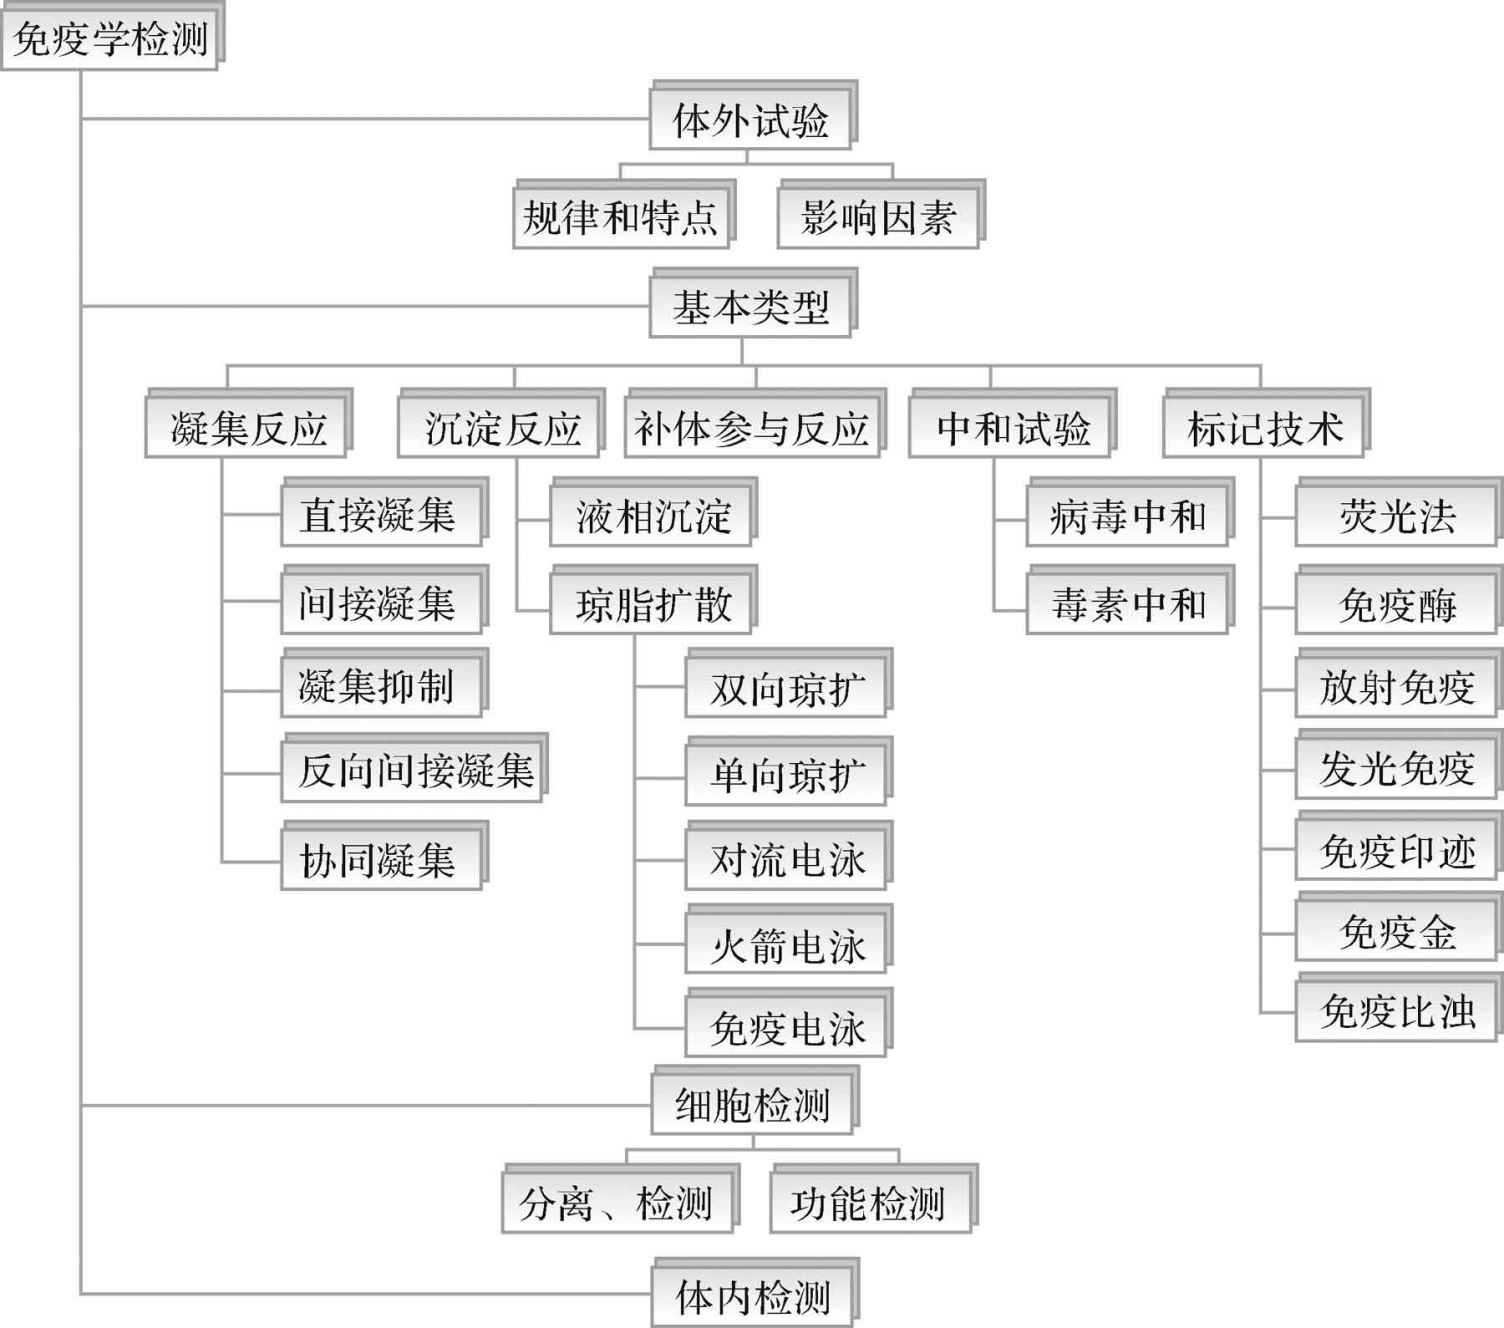
\includegraphics[width=.6\textwidth]{./images/Image00151.jpg}
\end{center}
\noindent\textbf{【课前思考】}

如果怀疑得了某种传染病或癌症,该如何确诊?机体对某种传染病有无抵抗力,该如何检测?对淋巴细胞(T细胞、B细胞、NK细胞)是如何鉴别的?如何诊断某人是否对青霉素过敏?是否得了结核病?

\noindent\textbf{【本章重点】}

1.免疫检测的基本原理、特点;

2.各类免疫检测的基本原理。

\noindent\textbf{【教学目标】}

1.掌握血清学试验的一般规律、影响因素;

2.掌握抗原或抗体检测常用的检测方法(凝集试验、沉淀试验、免疫标记技术等);

3.熟悉免疫细胞的分离、鉴定方法;

4.针对不同检测对象,能自主设计检测方法。
\end{framed}

免疫学检测是对抗原、抗体、免疫细胞数量、种类及其分化功能等进行定性或定量检测。免疫学检测技术在医学生物学研究领域得到广泛应用,并在临床医学中用于免疫相关疾病的诊断、病情监测、疗效评价等,本章介绍免疫学常用检测技术的基本原理、方法及其应用。

\section{检测抗原和抗体的体外试验}

抗原和抗体体外试验是指通过抗原与相应抗体在体外发生的特异性结合反应(凝集、沉淀等)来观察、分析、鉴定。抗体主要存在于血清中,这种体外的抗原-抗体反应又称血清学反应(试验)

抗原-抗体反应的检测技术主要应用于如下方面:

1.用已知抗原检测未知抗体。如临床上检测患者血清中抗病原微生物抗体、抗HLA的抗体、血型抗体以及各种自身抗体,用于诊断相关疾病;检测正常人群中注射某种疫苗后的抗体产生水平,来制订合理的免疫程序。

2.用已知抗体检测未知抗原。如检测各种病原微生物及其大分子产物,用于病原微生物的鉴定、分型、抗体O血型、HLA分型等。

3.血液学及免疫细胞的检测。用单克隆抗体检测血液细胞包括正常的和病理性的,进行免疫细胞的分类、鉴别等;抗血小板抗体及各种凝血因子的免疫学测定。

4.定性或定量检测体内各种大分子物质(如各种血清蛋白、可溶性血型物质、多肽类激素、细胞因子及肿瘤标志物AFP、CEA、PSA等),用于相关疾病的诊断或辅助诊断。

5.应用于内分泌检测(如HCG、LH、FSH、T3、T4等)、免疫因子(C3、C4、淋巴因子等)、用已知抗体检测某些药物、激素和炎性介质等各种半抗原物质,用于监测患者血清中药物浓度或运动员体内违禁药品水平等。


\subsection{血清学试验的一般规律和特点}

(一)用已知测未知

只有一种材料是未知的。

(二)试验和抑制试验

被相应的抗原或抗体所抑制,可以验证反应的特异性。

(三)特异性与交叉性

如变形杆菌与立克次氏体之间有共同的抗原决定簇,故斑疹伤寒病人血清可凝集OX19变形杆菌。为避免交叉反应干扰免疫学诊断,常采用吸收反应制备单价特异性抗血清,其原理是:将某一多价特异性抗血清与共同抗原(或称交叉抗原)反应,然后去除所形成的抗原抗体复合物。用颗粒性抗原进行的吸收反应,称为凝集吸收反应。

(四)抗原-抗体的结合比例与“带现象”

若抗原-抗体的数量比例合适,抗体分子的两个Fab段分别与两个抗原决定簇结合,相互交叉形成体积大、数量多,肉眼可见的网格状复合体,基本不存在游离的抗原或抗体,即抗原-抗体反应的等价带,此时形成肉眼可见的反应物(沉淀物或凝集物)。

在抗原-抗体反应中,可能出现抗原或抗体过剩的情况,由于过剩一方的结合价不能被完全占据,多呈游离的小分子复合物形式,或所形成的复合物易解离,不能被肉眼察见------“带现象”(图\ref{fig10-1})。

抗体过剩------前带,抗原过剩------后带,在检测中,应注意对抗原和抗体的浓度、比例进行适度的调整。

\begin{figure}[!htbp]
 \centering
 
\includegraphics[width=.6\textwidth]{./images/Image00152.jpg}
 \captionsetup{justification=centering}
 \caption{带现象示意图}
 \label{fig10-1}
  \end{figure} 

(五)特异性结合与反应可见两个阶段

第一阶段:抗原-抗体特异性结合。特点:反应快,几秒~几分钟内完成,无肉眼可见的反应。

第二阶段:反应可见阶段。特点:出现凝集、沉淀、细胞溶解等现象,时间几分钟~几天,受电解质、温度、pH等影响。

(六)可逆性

抗原与抗体为分子表面的非共价结合复合物,结合虽稳定但可逆;在一定条件下,可解离为游离的抗原、抗体,解离后的抗原和抗体仍保持原有的理化特性及生物学性状。


\subsection{抗原-抗体反应的影响因素}

(一)电解质

抗原-抗体有对应的极性基团,能相互吸附并由亲水性变为疏水性。电解质的存在使抗原-抗体复合物失去电荷而凝聚,出现可见反应,故免疫学试验中多用0.9\%氯化钠稀释抗原或抗体。

(二)酸碱度

抗原-抗体反应的最适pH是6~8。超出此范围可影响抗原、抗体的理化性状,出现假阳性或假阴性。

(三)温度

适当的温度可增加抗原与抗体分子碰撞的机会,加快二者结合速度,其最适温度为37℃。某些抗原-抗体反应有其独特的最适温度,如冷凝集素在4℃左右与红细胞结合最好,20℃以上反而解离。此外,适当震荡或搅拌也可促进抗原-抗体分子的接触,提高结合速度。

(四)抗原-抗体的性质

抗体的特异性和亲和力是决定抗原-抗体反应的关键因素。从免疫早期动物所获抗血清其亲和力一般较低,而后期所得抗血清一般亲和力较高;单克隆抗体亲和力较低,一般不适用于低灵敏度的沉淀反应和凝集反应。此外,抗原理化性质、抗原决定簇多寡和种类等均可影响抗原-抗体反应。

抗原-抗体的浓度、比例对抗原-抗体反应的影响最大,是决定性因素。

\section{抗原-抗体反应的基本类型}

根据抗原的性质、结合反应的现象、参与反应的成分等因素,可将基于抗原-抗体反应的检测方法分为凝集反应、沉淀反应、补体参与的反应、中和反应以及免疫标记技术等。


\subsection{凝集反应(agglutination)}

细菌、红细胞等颗粒性抗原与相应抗体结合后,在一定条件下出现肉眼可见的凝集物,此为凝集反应。

(一)直接凝集反应

细菌或红细胞与相应抗体直接反应,可出现细菌或红细胞凝集现象(图\ref{fig10-2})。

1.玻片法:定性

其方法为:①已知抗体与相应抗原在玻片上反应,用于抗原的定性检测(如ABO血型鉴定、细菌鉴定)。

\begin{figure}[!htbp]
 \centering
 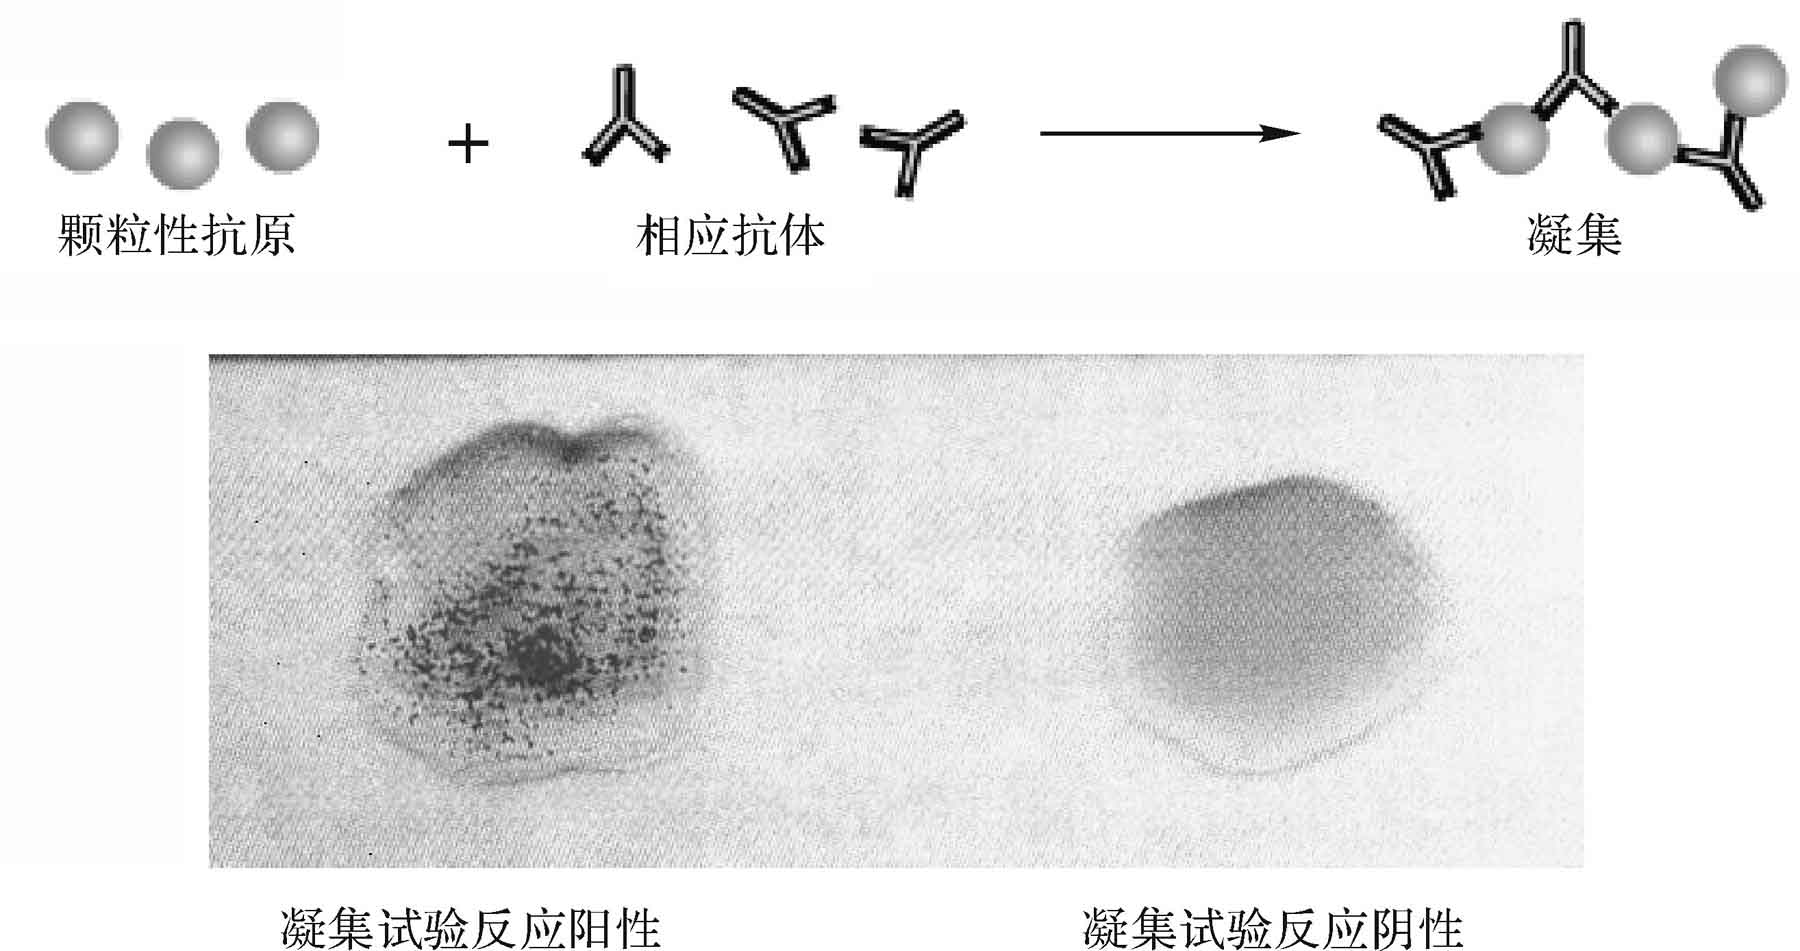
\includegraphics{./images/Image00153.jpg}
 \captionsetup{justification=centering}
 \caption{直接凝集反应示意图}
 \label{fig10-2}
  \end{figure} 

2.试管法:定量

多用已知抗原测未知抗体的相对含量,如:诊断伤寒、副伤寒、布氏杆菌病。

方法:待检血清在试管内用0.9\%氯化钠倍比稀释,加入等量菌液,37℃,数小时观察结果(表\ref{tab10-1})。
 
\begin{table}[htbp]
    \centering
    \caption{试管倍比稀释法测定待检血清效价}
    \label{tab10-1}
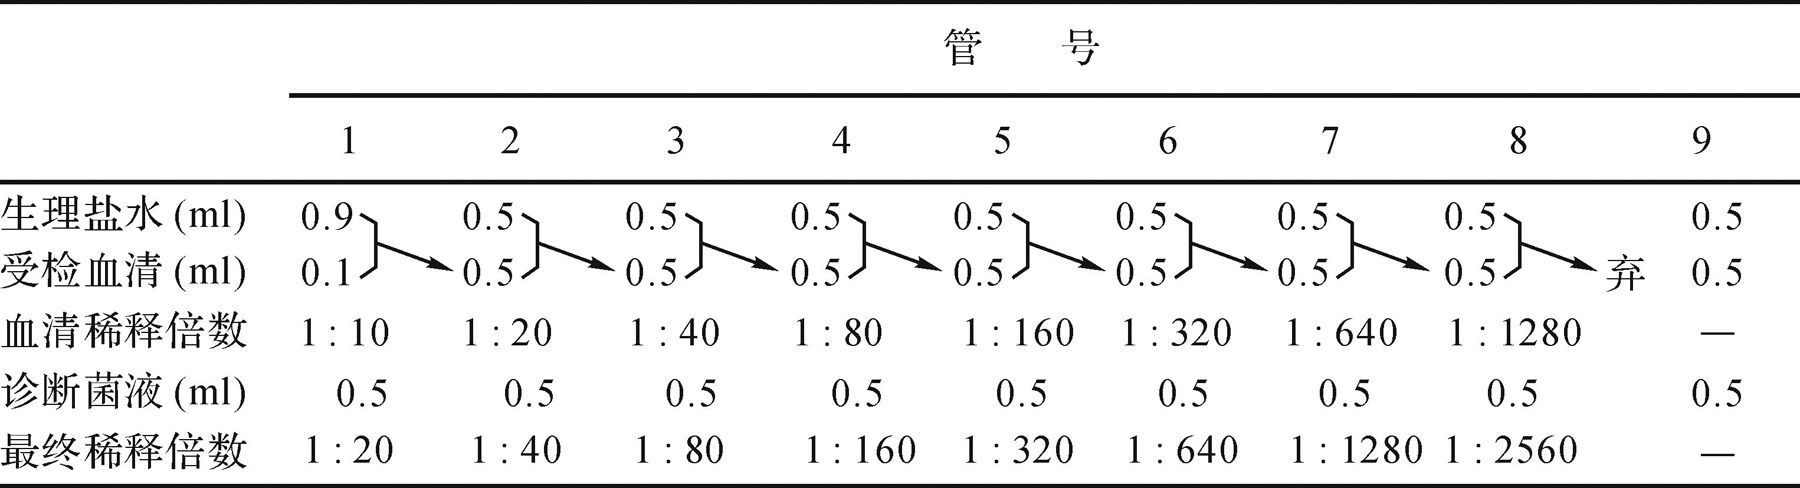
\includegraphics[width=.8\textwidth]{./images/Image00154.jpg}
\end{table}

观察每个试管内抗原的凝集程度,凝集分五级:

(1)++++:很强,细菌全部凝集,管内液体澄清,可见管底有大片边缘不整的白色凝集物,轻摇时可见明显的颗粒、薄片或絮状。

(2)+++:强,细菌大部分凝集,液体较混浊,管底有边缘不整的白色凝集物,轻摇时也可见明显的颗粒、薄片或絮状。

(3)++:中等强度,细菌部分凝集,液体较混浊,管底有少量凝集物呈颗粒状。

(4)+:弱,细菌仅有少量凝集,液体混浊,管底凝集呈颗粒状,小不易观察。

(5)-:不凝集,液体混浊度、管底沉积物同对照管相似。

通常以出现明显凝集现象(++)的血清最高稀释度为该血清的抗体效价。

(二)间接凝集反应

该反应将可溶性抗原包被在与免疫无关的载体颗粒表面,再与相应抗体反应,出现颗粒物凝集现象(图\ref{fig10-3})。常用载体为人O型血红细胞、聚苯乙烯乳胶颗粒等。用途:检测血清中的自身抗体和抗微生物的抗体。

\begin{figure}[!htbp]
 \centering
 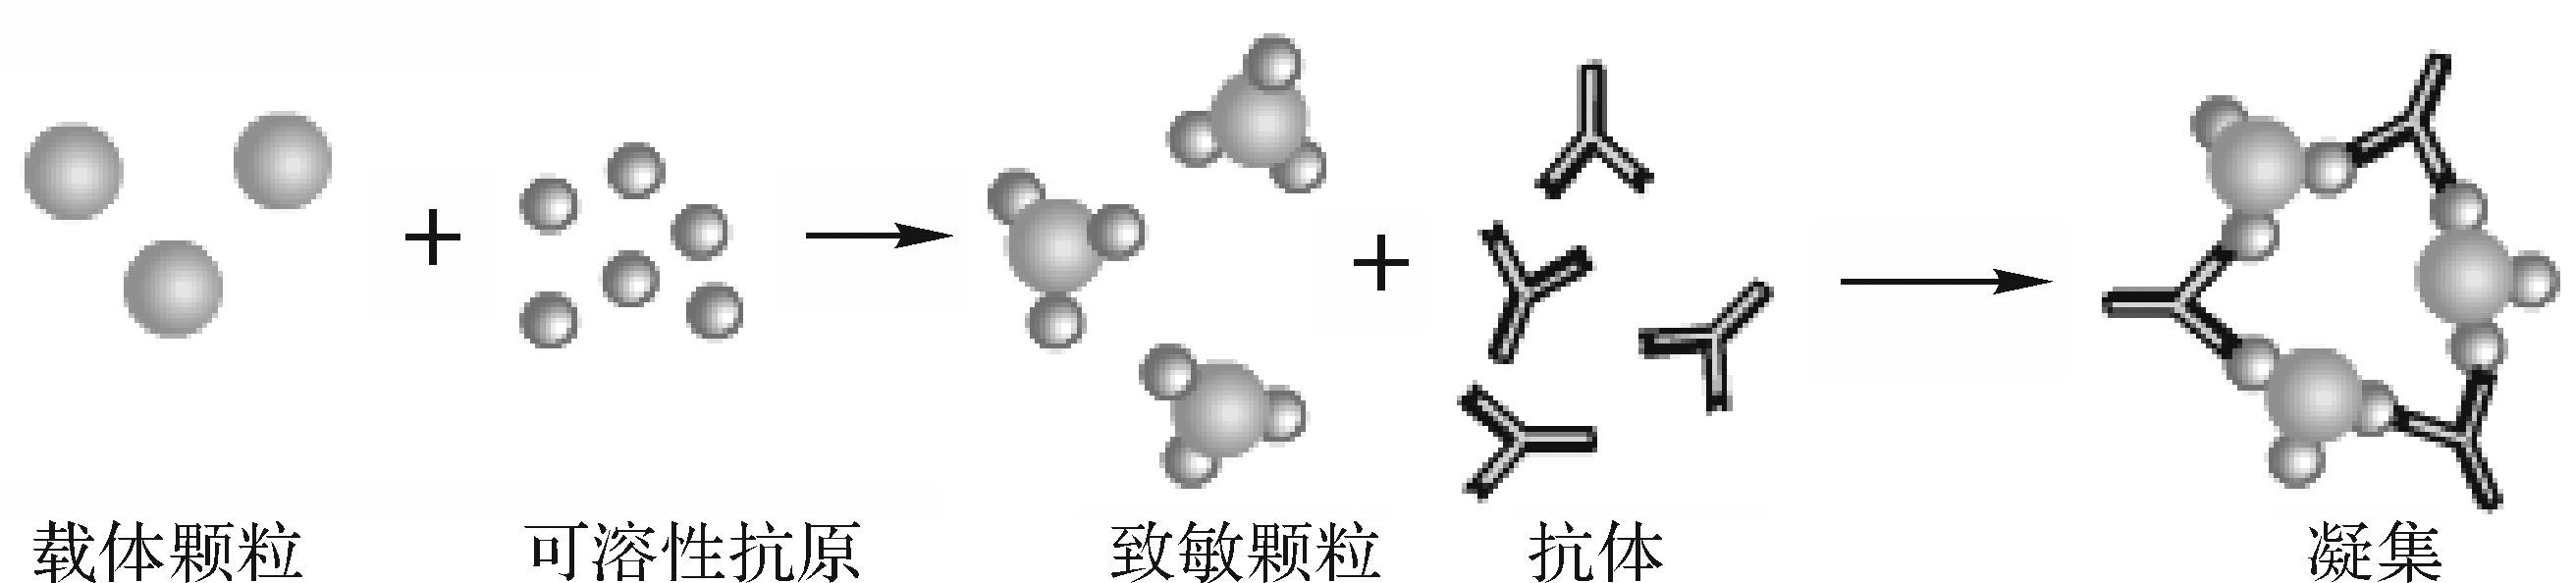
\includegraphics{./images/Image00155.jpg}
 \captionsetup{justification=centering}
 \caption{间接凝集反应示意图}
 \label{fig10-3}
  \end{figure} 

(三)间接凝集抑制试验

其原理是:将待测抗原(或抗体)与特异性抗体(或抗原)先行混合并作用一定时间,再加入相应致敏载体悬液;若待测抗原与抗体对应,即发生中和,随后加入的相应致敏载体颗粒不再被凝集,使本应出现的凝集现象被抑制,故得名(图\ref{fig10-4})。此试验可用于检测抗原或抗体(如早孕的检测),其灵敏度高于一般间接凝集试验;可用来检测可溶性抗原,如免疫妊娠诊断试验。

(1)诊断抗原:HCG致敏的乳胶颗粒;

(2)诊断血清:抗HCG的抗体;

(3)检测标本:尿液(是否含有HCG)。

\begin{figure}[!htbp]
 \centering
 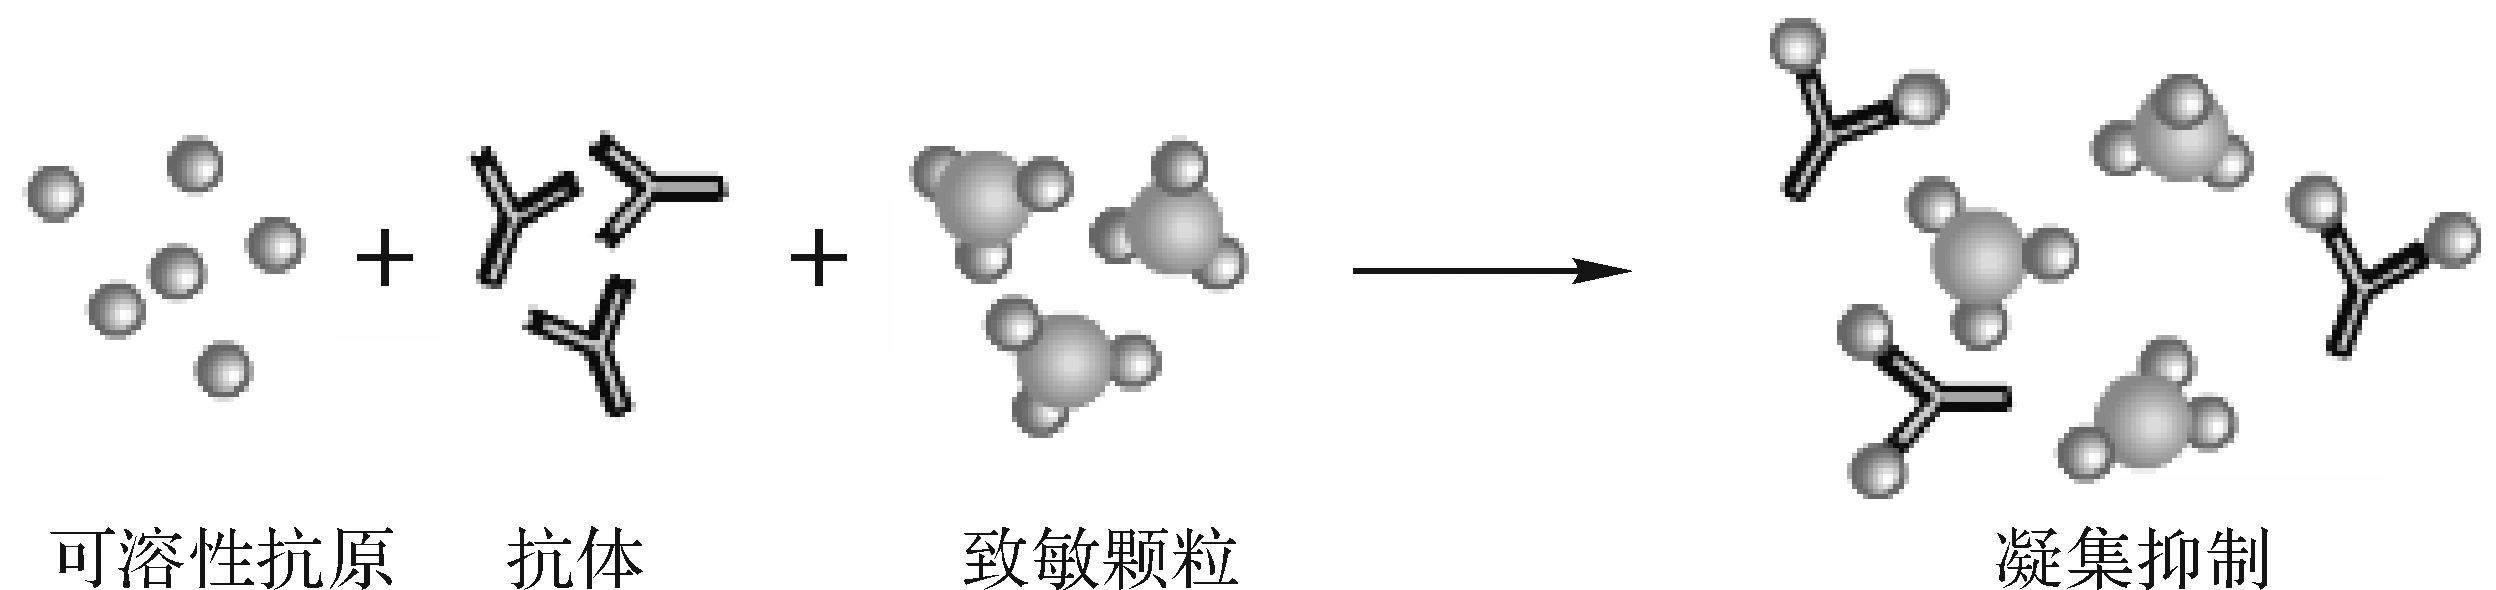
\includegraphics{./images/Image00156.jpg}
 \captionsetup{justification=centering}
 \caption{间接凝集抑制反应示意图}
 \label{fig10-4}
  \end{figure} 

(四)反向间接凝集试验

反向间接凝集试验是用特异性抗体致敏载体,检测标本中的相应抗原的反应(图\ref{fig10-5}),可用于检测乙型肝炎病毒表面抗原、甲胎蛋白、新型隐球菌荚膜抗原等。

\begin{figure}[!htbp]
 \centering
 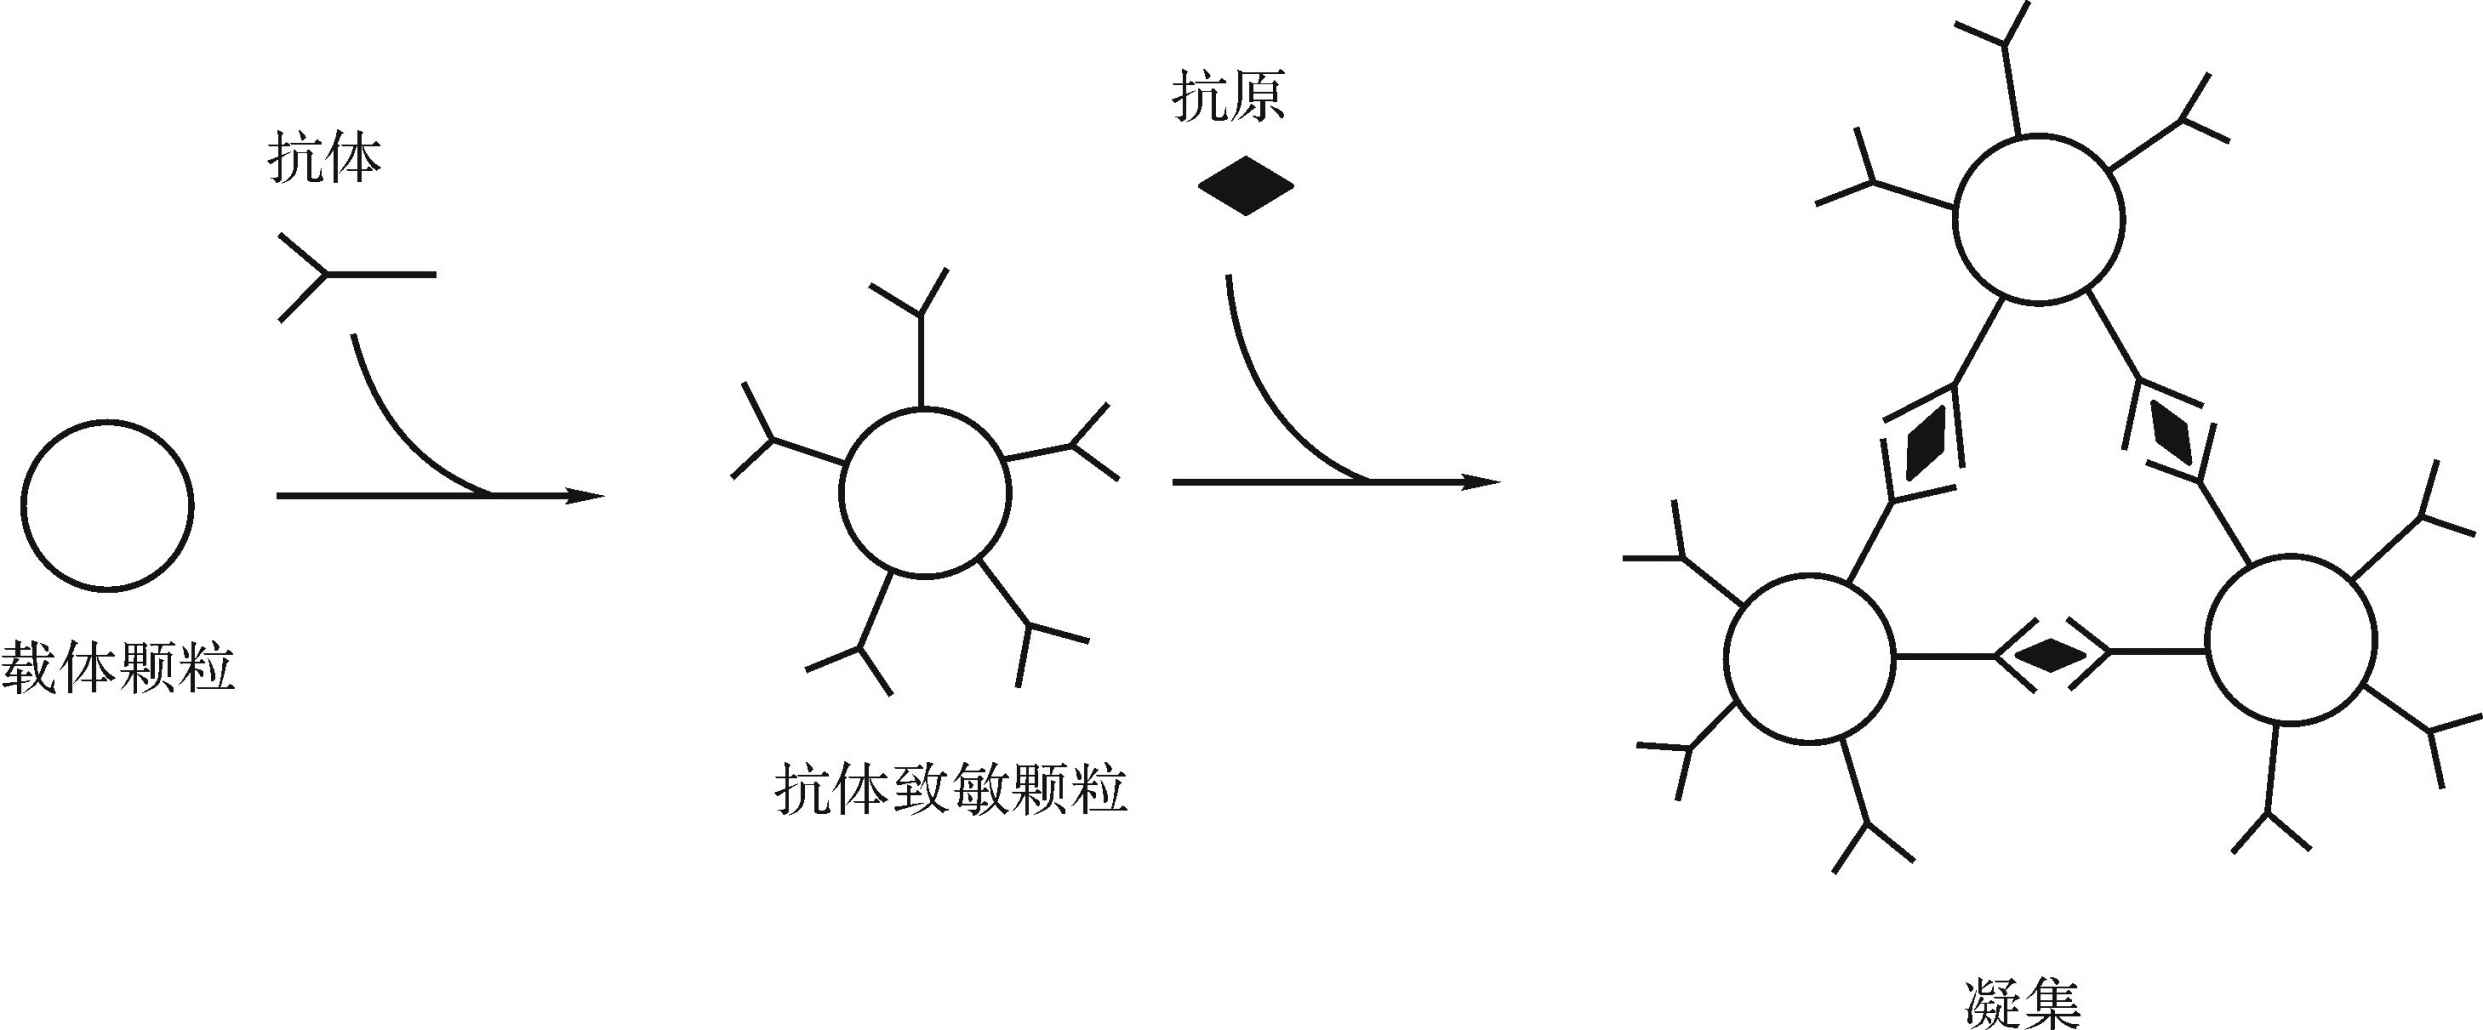
\includegraphics{./images/Image00157.jpg}
 \captionsetup{justification=centering}
 \caption{反向间接凝集试验示意图}
 \label{fig10-5}
  \end{figure} 

(五)协同凝集试验

协同凝集试验(COAG)的原理是:金黄色葡萄球菌细胞壁成分蛋白A(SPA)能与人和多种哺乳动物血清中的IgG分子的Fc片段结合,Fab就暴露,能与相应抗原结合,产生协同凝集反应(图\ref{fig10-6})。本试验通常可用于检测传染病患者的血液、脑脊液和其他分泌物中可能存在的微量可溶性抗原,目前已用于流行性脑脊髓膜炎(简称流脑)、伤寒、布氏菌病的早期诊断。

\begin{figure}[!htbp]
 \centering
 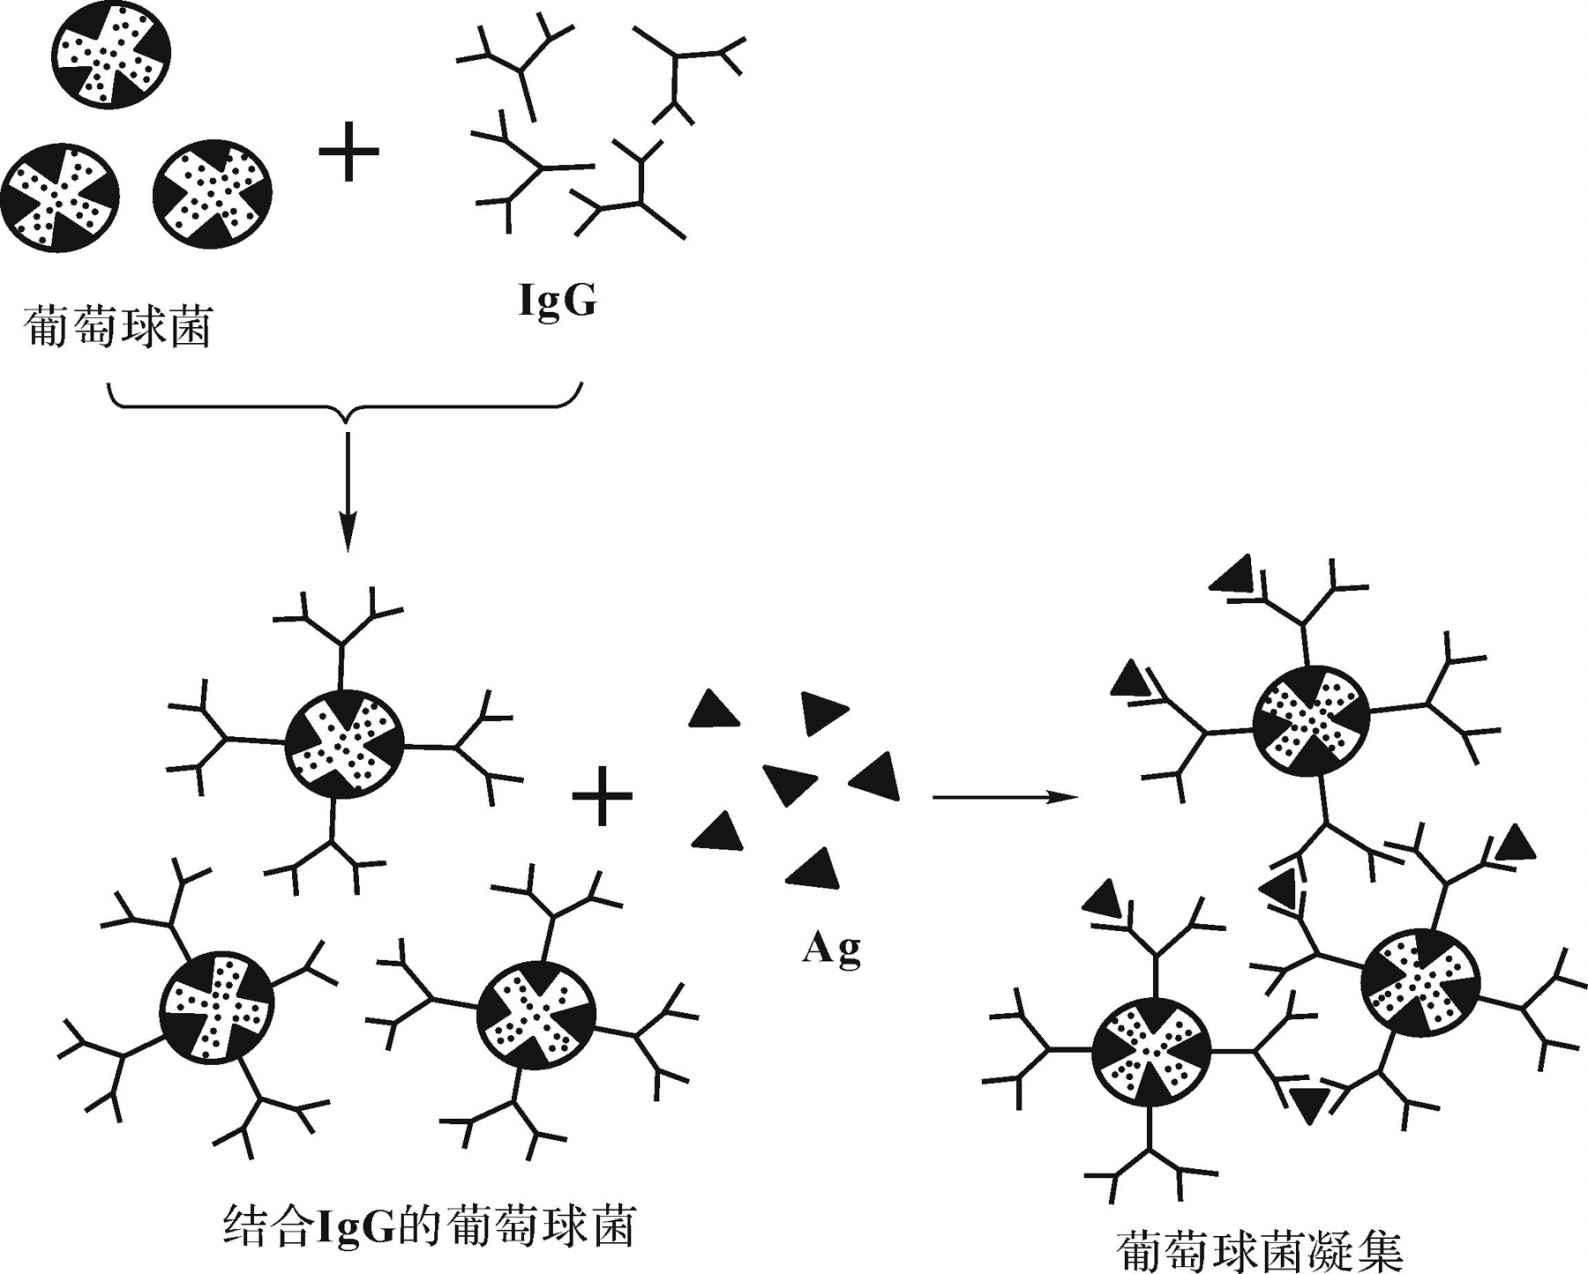
\includegraphics{./images/Image00158.jpg}
 \captionsetup{justification=centering}
 \caption{协同凝集试验示意图}
 \label{fig10-6}
  \end{figure} 


\subsection{沉淀反应}

沉淀反应(precipitation)是将可溶性抗原(沉淀原)与相应抗体(沉淀素)结合后,在一定条件下出现肉眼可见的沉淀,此为沉淀反应。该反应多用半固体琼脂凝胶作为介质进行琼脂扩散或免疫扩散,即可溶性抗原与抗体在凝胶中扩散,在比例合适处相遇即形成可见的白色沉淀。

沉淀原:内、外毒素,菌体裂解液、血清、蛋白质、多糖、类脂等,其体积小,与抗体相比反应面积大,故试验时需对抗原进行稀释,以避免沉淀原过剩出现后带现象,并以抗原稀释度作为沉淀试验的效价。

(一)液相沉淀试验------环状沉淀试验

已知抗血清+待检抗原→液面交界处,白色环状沉淀“+”,可用来鉴别血迹性质、测定媒介昆虫的嗜血性、鉴定某些细菌。

(二)琼脂扩散试验

用半固体琼脂凝胶作为介质进行琼脂扩散或免疫扩散,即可溶性抗原与抗体在凝胶中扩散,在比例合适处相遇即形成可见的白色沉淀。

1.双向免疫扩散

双向免疫扩散(double immunodiffusion)
是将抗原和抗体分别加入琼脂凝胶的小孔中,二者自由向四周扩散,在相遇处形成沉淀线。若反应体系中含两种以上抗原-抗体系统,则小孔间可出现两条以上沉淀线(图\ref{fig10-7})。特点:敏感性不高,所需时间较长。用于:

\begin{figure}[!htbp]
 \centering
 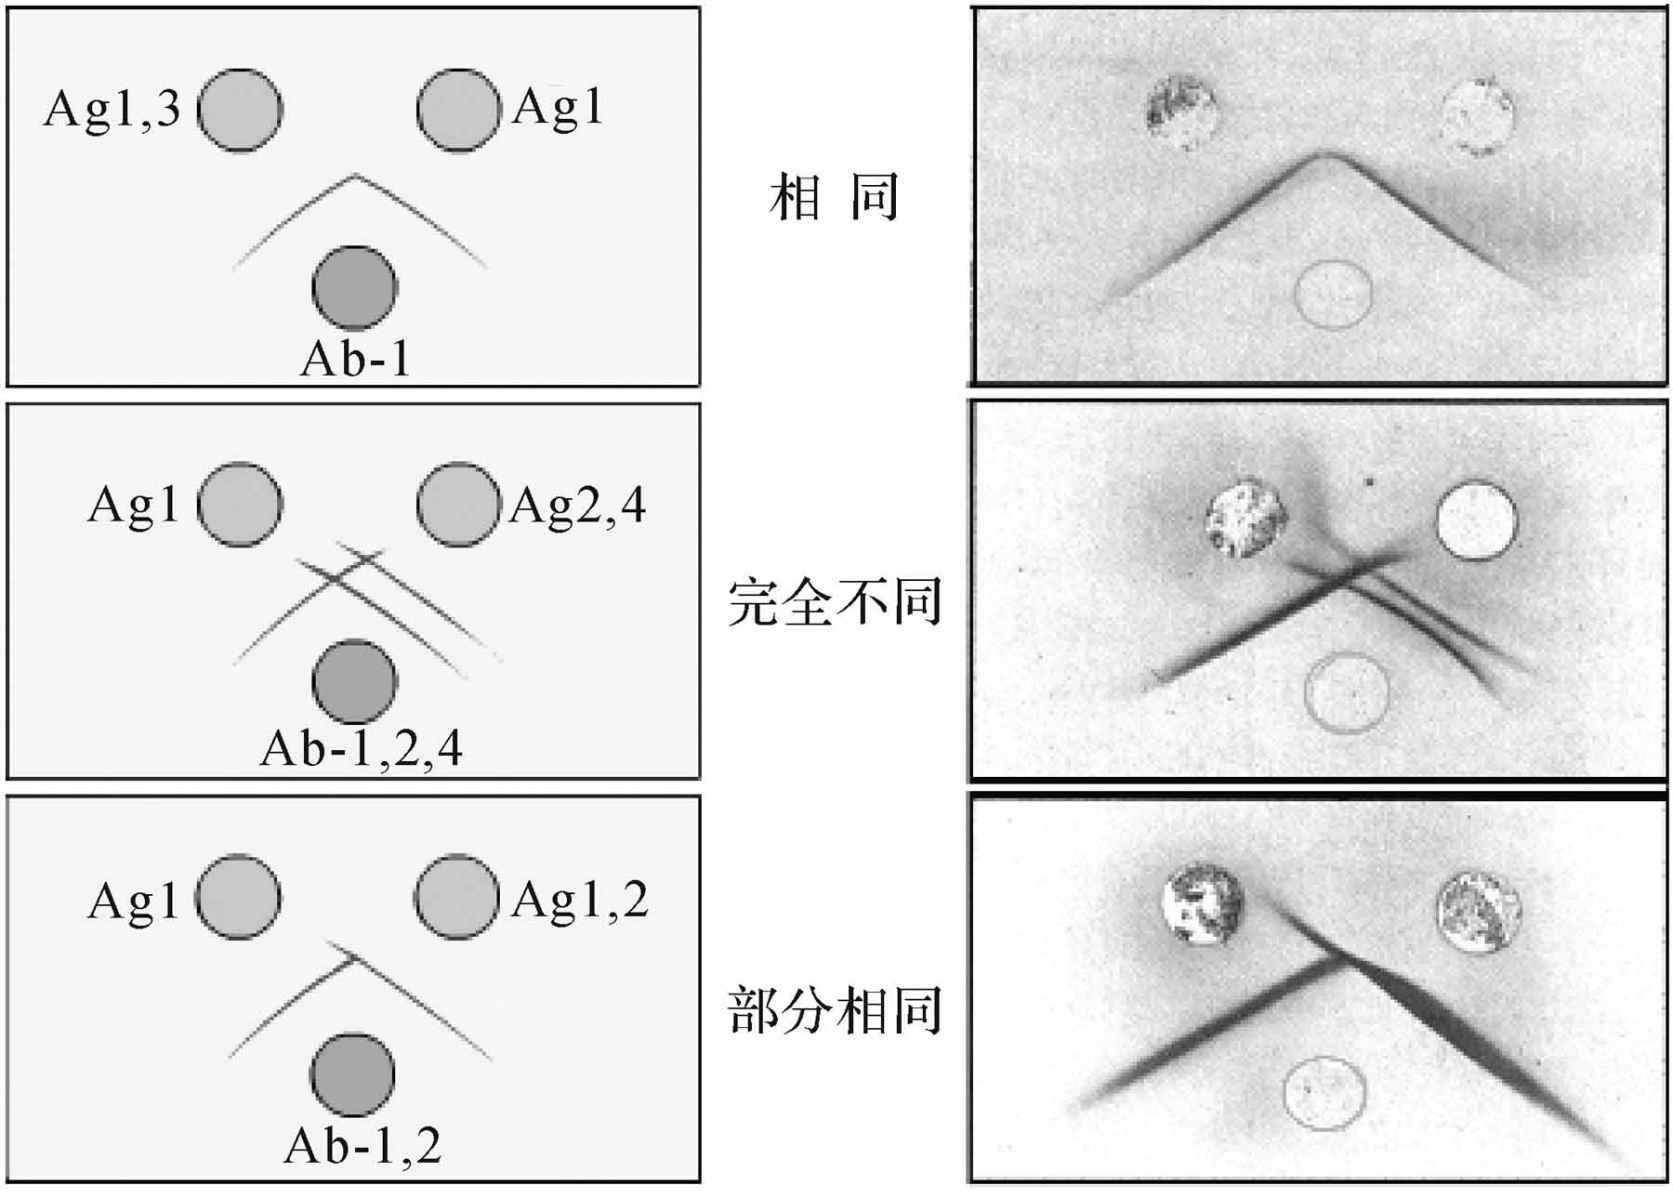
\includegraphics{./images/Image00159.jpg}
 \captionsetup{justification=centering}
 \caption{双向琼脂扩散试验示意图}
 \label{fig10-7}
  \end{figure} 

(1)定性检测可溶性抗原或抗体。

(2)对复杂的抗原成分或抗原、抗体的提取纯度进行分析鉴定。

(3)测定免疫血清的效价。

2.单向免疫扩散

单向免疫扩散(single
immunodiffusion)是将一定量已知抗体混于琼脂凝胶(45℃)中制成琼脂板,在适当位置打孔并加入抗原。抗原在扩散过程中与凝胶中的抗体相遇,形成以抗原孔为中心的沉淀环,环的直径与抗原含量呈正相关。取已知量抗原绘制标准曲线,可根据所形成沉淀环的直径,从标准曲线中查出待检标本的抗原含量(图\ref{fig10-8})。

\begin{figure}[!htbp]
 \centering
 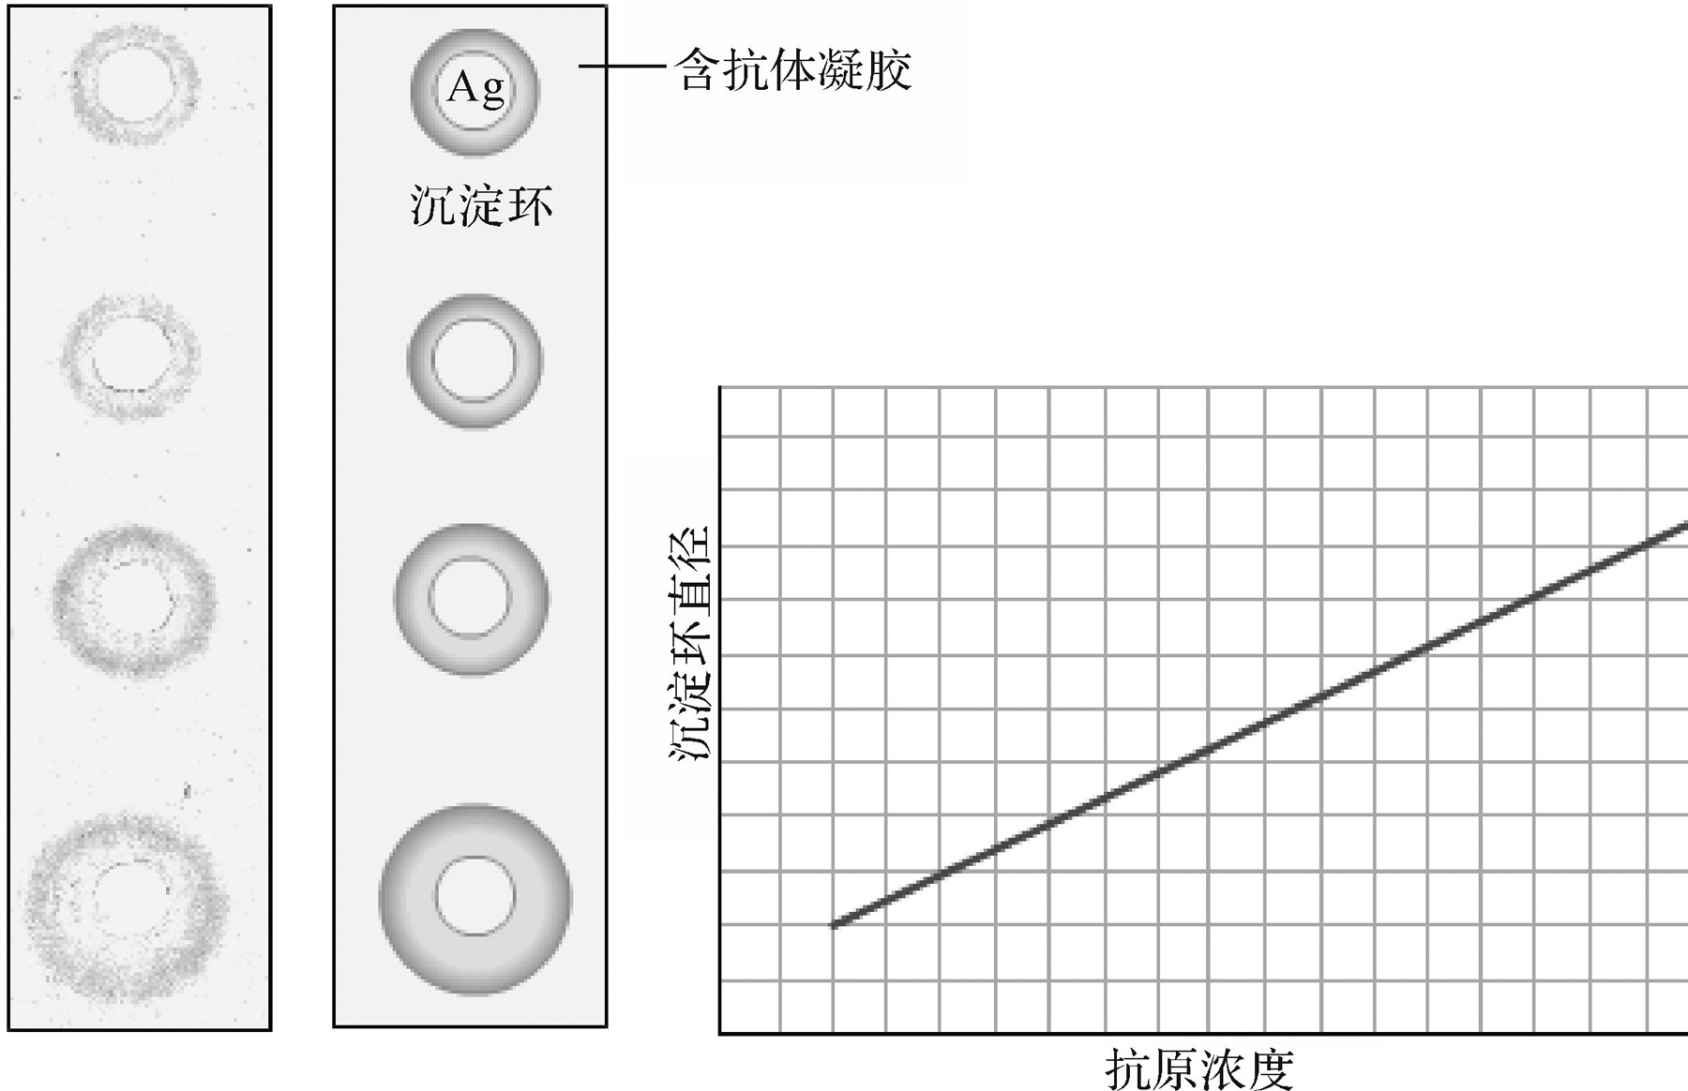
\includegraphics{./images/Image00160.jpg}
 \captionsetup{justification=centering}
 \caption{单向琼脂扩散试验示意图}
 \label{fig10-8}
  \end{figure} 

3.对流免疫电泳

对流免疫电泳(CIE)又称免疫电渗电泳,双向琼脂扩散与电泳技术相结合。试验在装有pH8.6缓冲液的电泳槽中进行(图\ref{fig10-9})。

\begin{figure}[!htbp]
 \centering
 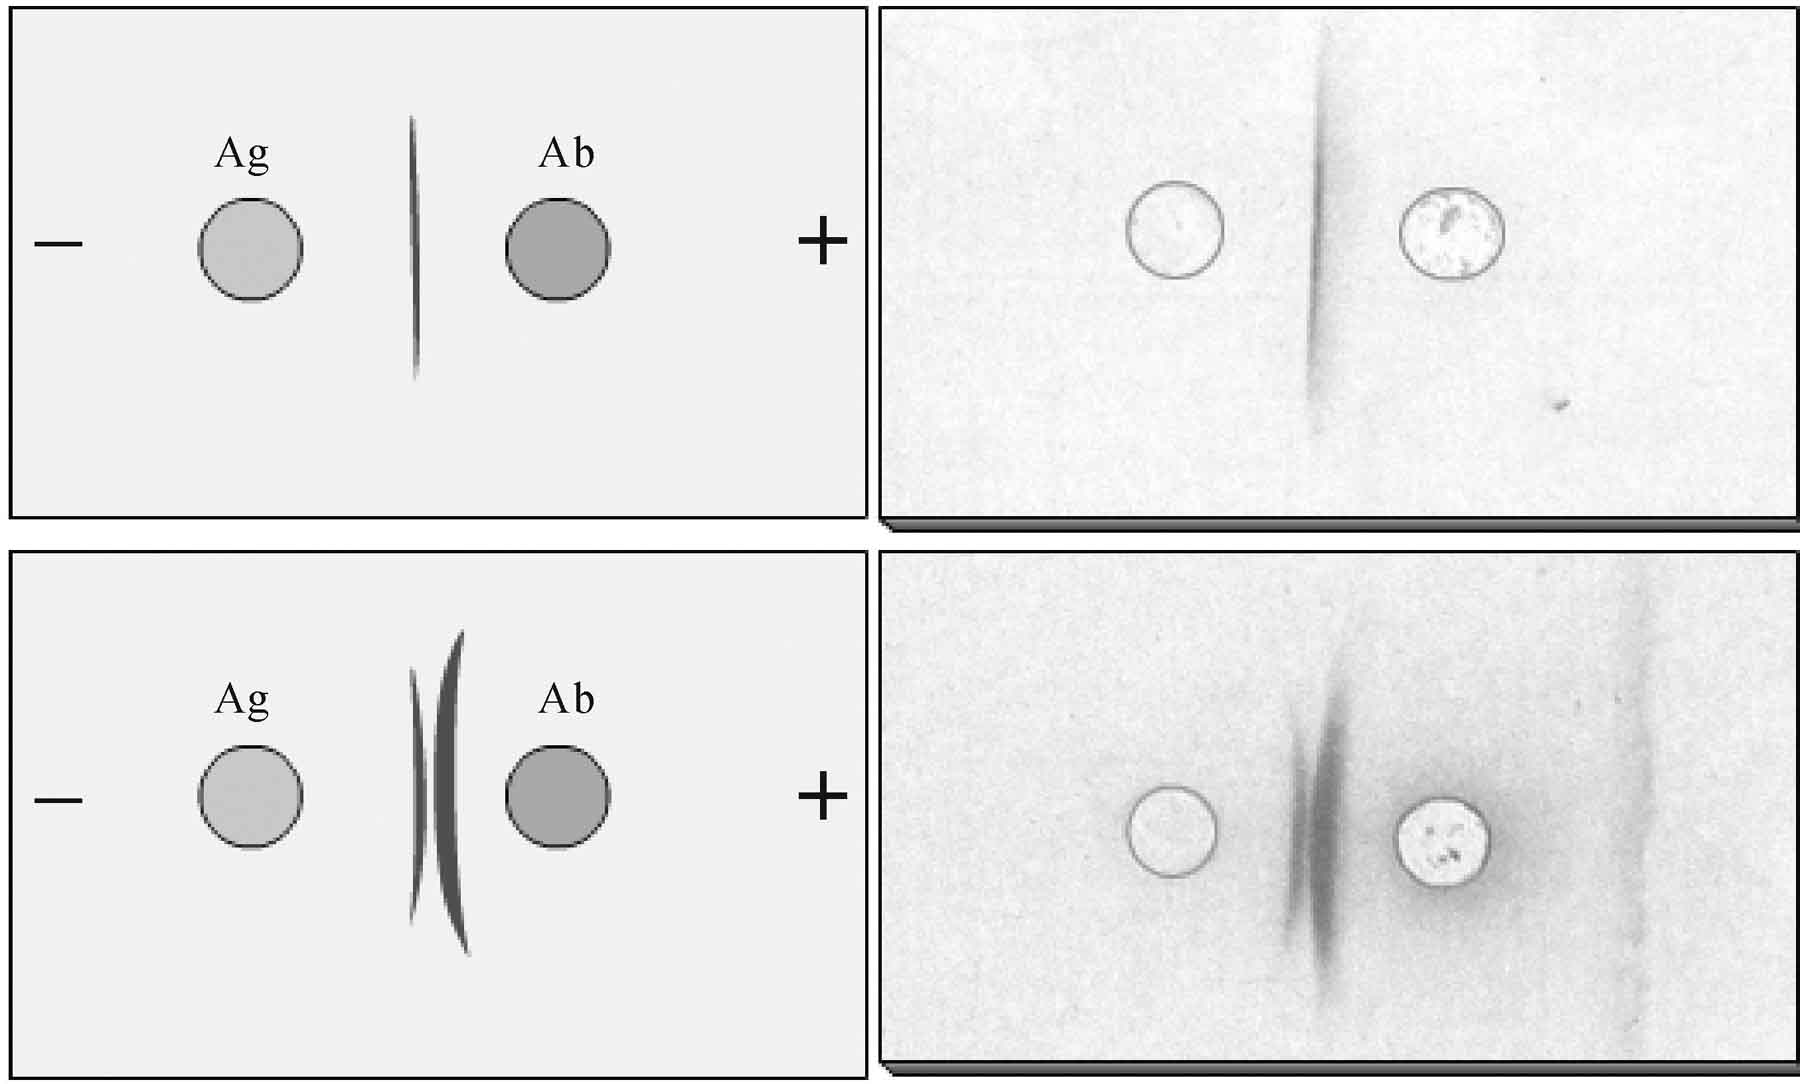
\includegraphics{./images/Image00161.jpg}
 \captionsetup{justification=centering}
 \caption{对流免疫电泳试验示意图}
 \label{fig10-9}
  \end{figure} 

(1)原理:抗原和抗体在电泳时受两种作用力的影响,一种是电场力,使抗原和抗体由“-”极向“+”极移动;另一种是电渗力,使抗原和抗体由“+”极向“-”极移动。

通常,抗原等电点偏低(pH 4~5),在碱性缓冲液(pH
8.6)中所带负电荷较多,受电场力较大,而其相对分子质量较小,所受电渗作用影响小,合力结果是电场力大于电渗力。因此,通电后,抗原由“-”极向“+”极移动。

抗体为球蛋白,等电点偏高(pH
6~7),所带负电荷较少,受电场力影响较小,而其相对分子质量较大,所受电渗作用影响大,合力结果电渗力大于电场力。因此,通电后,抗体由“+”极向“-”极移动。

两者相对而行,缩短了反应时间,提高了试验的敏感性。

(2)特点:操作简便,敏感性高,所需时间短。本试验可用来检测血清中的HBsAg和AFP等可溶性抗原。

(3)方法:将抗原和抗体分别加入琼脂板孔中,通电进行电泳[4mA/cm(宽)端电压:6V/cm
],电泳45~60min,水洗和洗色。

4.火箭电泳

火箭电泳又称电泳免疫扩散,单向琼脂扩散与电泳结合。本试验的敏感性与单向琼脂扩散相当,但所需时间短,故可用来测定标本中可溶性抗原的含量(图\ref{fig10-10})。

试验时,将适当浓度的已知抗体加入融化(45℃)的琼脂中,混匀后浇注于玻璃板,制成凝胶板,将抗原加入孔中,在盛有pH8.6缓冲液的电泳槽中电泳,电流强度3mA/cm(或电压10V/cm),电泳时间2~10h。电泳后在比例最适处形成锥形沉淀峰。

\begin{figure}[!htbp]
 \centering
 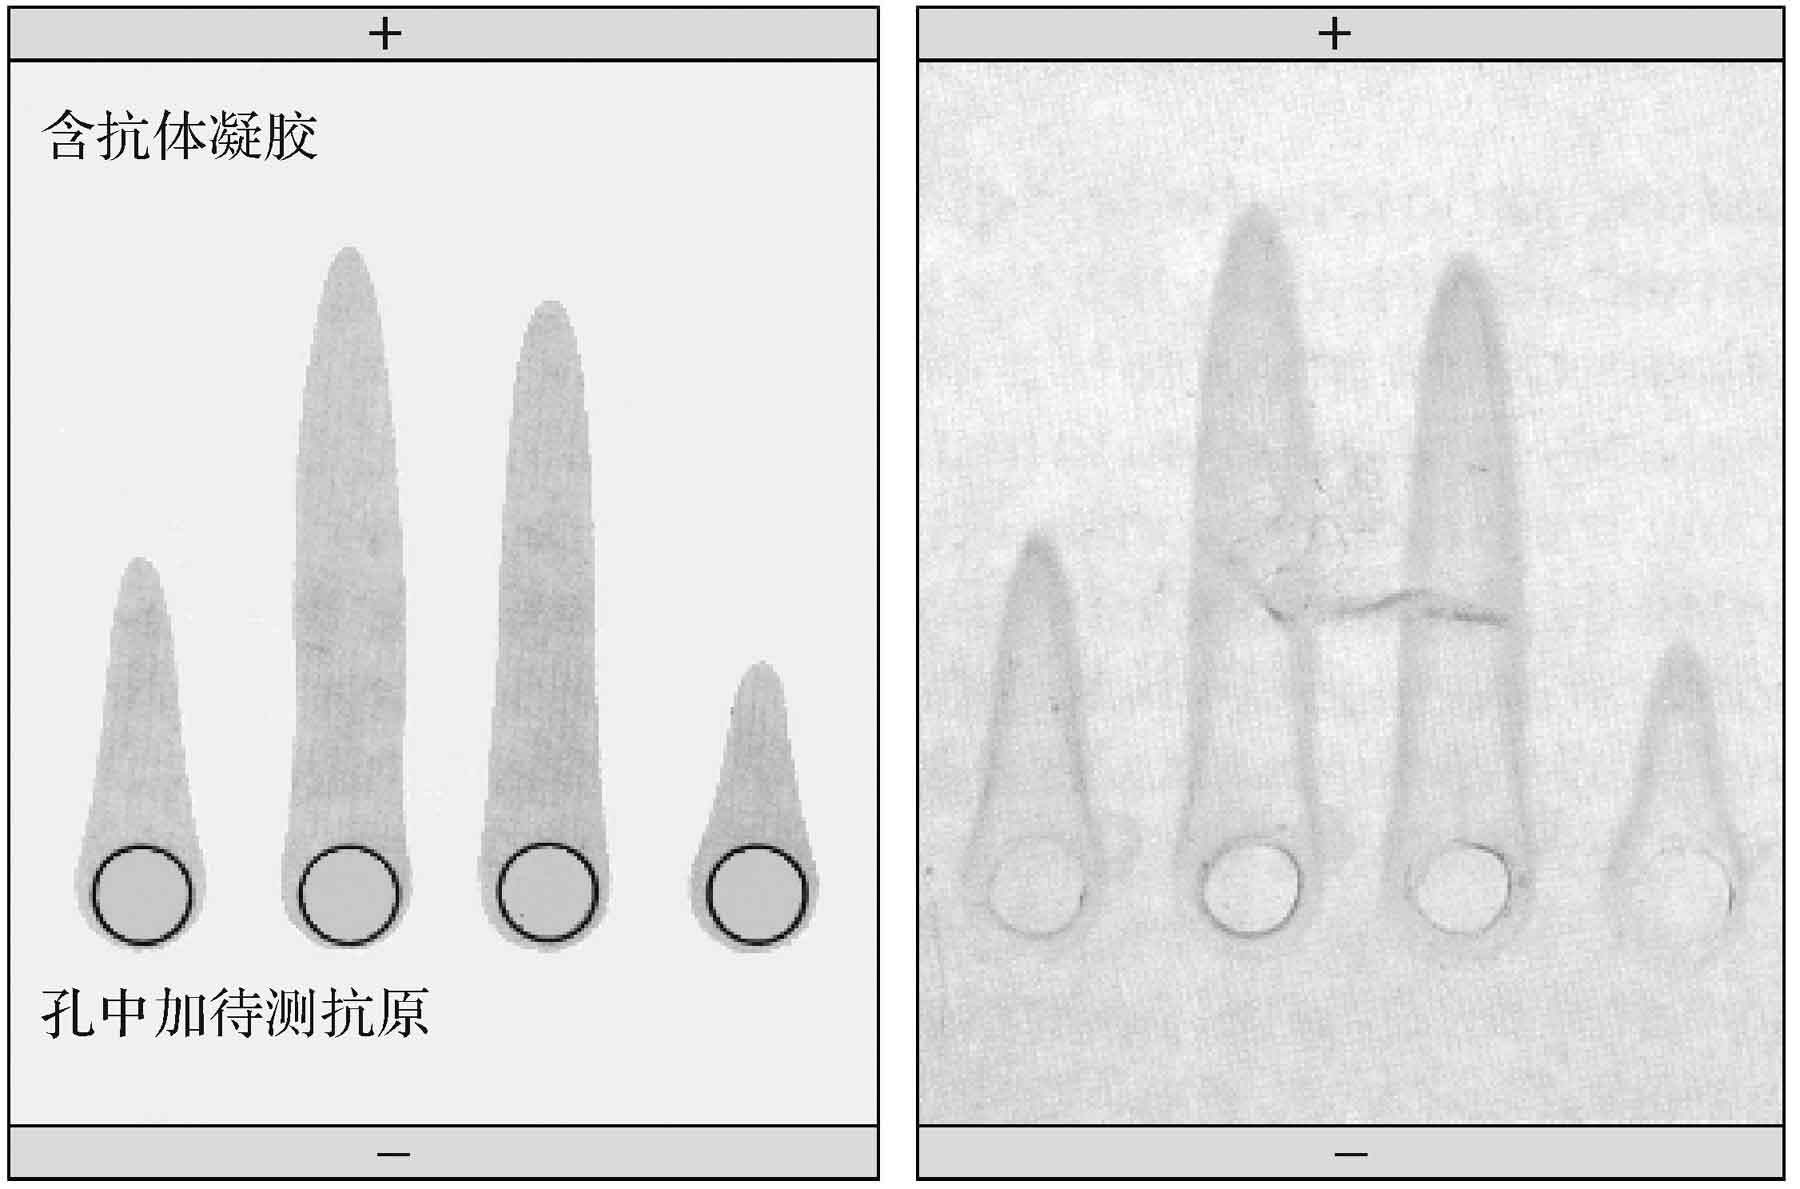
\includegraphics{./images/Image00162.jpg}
 \captionsetup{justification=centering}
 \caption{火箭免疫电泳试验示意图}
 \label{fig10-10}
  \end{figure} 

5.免疫电泳

免疫电泳(immunoelectrophoresis)
是将琼脂电泳与双向琼脂扩散结合的技术。待检标本在孔内先电泳,各种成分分开。之后挖槽,加入相应抗体,进行双向琼脂扩散。

根据沉淀弧的数量、位置、形状,并通过与已知标准抗原相比,可对样品中所含成分及其性质作出判断(图\ref{fig10-11})。

本试验样品用量小、特异性高、分辨力强,主要用于血清蛋白及抗体成分的分析研究,亦可用于抗原或抗体提取物的纯度鉴定。

\begin{figure}[!htbp]
 \centering
 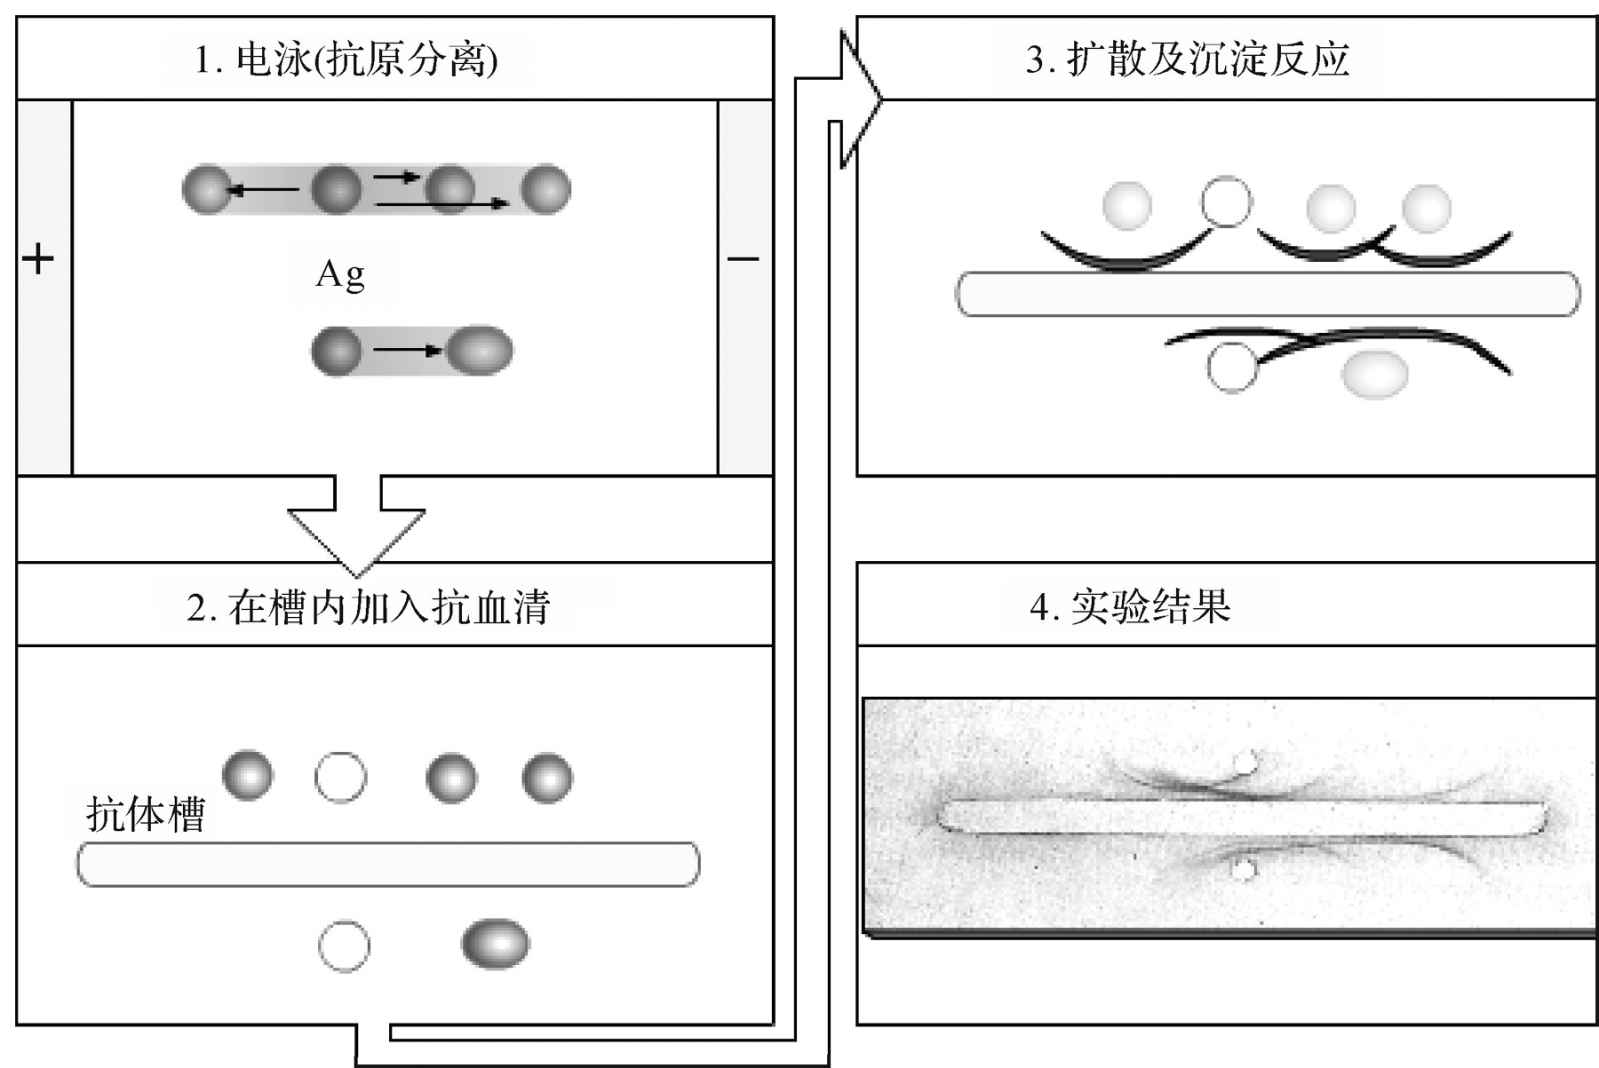
\includegraphics[width=.6\textwidth]{./images/Image00163.jpg}
 \captionsetup{justification=centering}
 \caption{免疫电泳试验示意图}
 \label{fig10-11}
  \end{figure} 


\subsection{补体参与的反应}

1.溶菌反应:细菌与相应抗体结合,可激活补体,使细菌溶解,主要发生于霍乱弧菌等G\textsuperscript{+}
菌,可用于细菌鉴定。

2.溶血反应:红细胞与相应抗体结合,通过激活补体使红细胞溶解,可作为补体结合试验的指示系统。

3.补体结合反应:是一种在补体参与的条件下,以绵羊红细胞和溶血素作为指示系统来测定有无相应抗原或抗体的血清学试验(图\ref{fig10-12})。

\begin{figure}[!htbp]
 \centering
 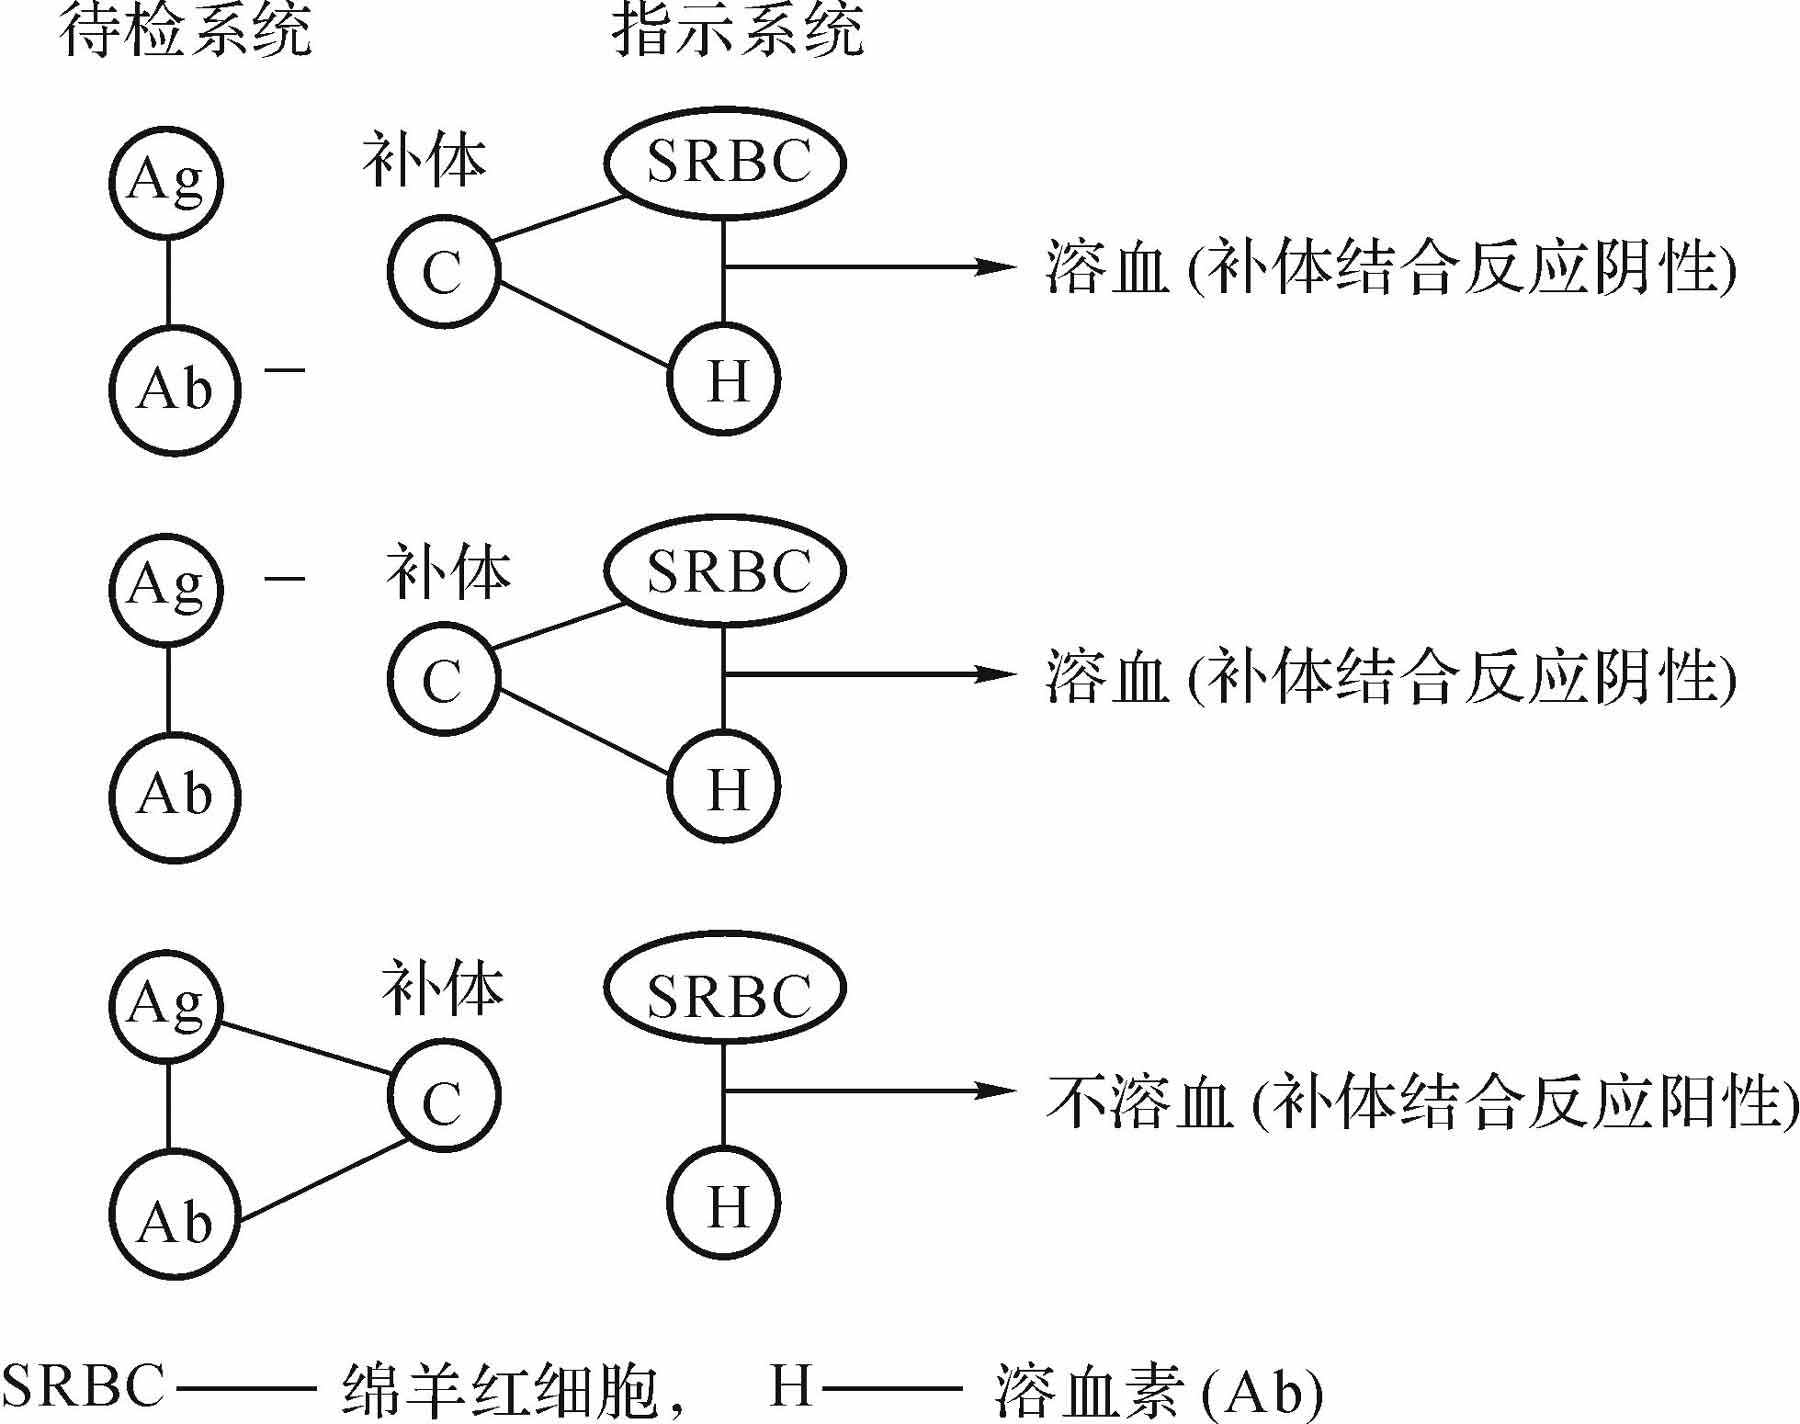
\includegraphics[width=.6\textwidth]{./images/Image00164.jpg}
 \captionsetup{justification=centering}
 \caption{补体结合反应示意图}
 \label{fig10-12}
  \end{figure} 


\subsection{中和试验}

毒素、酶、激素和病毒等与相应抗体(中和抗体)结合,使之丧失生物学活性的现象称为中和反应。

1.病毒中和试验

病毒中和试验是病毒在活体内或细胞培养中被特异性抗体中和而失去感染性的一种试验。检查患病后或人工免疫后机体血清中相应中和抗体的增长情况,也可用来鉴定病毒。

2.毒素中和试验

外毒素与相应抗毒素结合后丧失其毒性,分体内和体外两种。

如:抗链球菌溶血素O试验。

乙型溶血性链球菌→溶血素(可溶解人、兔红细胞)→刺激机体产生抗毒素(抗体)。溶血素+抗体→毒性丧失,不溶血。

病人血清(未知)+溶血素O(经一定时间)+人红细胞→红细胞不溶解破坏------待检血清中有相应抗体,试验“+”。

本试验常用于临床风湿病的辅助诊断。


\subsection{免疫标记技术}

免疫标记技术(immunolabelling
technique)是用荧光素、酶、放射性核素或化学发光物质等标记抗体或抗原,进行抗原-抗体反应的检测。标记物与抗体或抗原连接后并不改变抗原-抗体的免疫特性,具有灵敏度高、快速、可定性、定量、定位等优点。

(一)免疫荧光法(immunofluorescence,IF)

免疫荧光法又称荧光抗体技术,用荧光素与抗体连接成荧光抗体,再与待检标本中抗原反应,置荧光显微镜下观察,抗原-抗体复合物散发荧光,借此对抗原进行定性或定位。

荧光素包括:异硫氰酸荧光素(FITC)(黄绿色荧光)、四乙基罗丹明(RB200)(橙色荧光)、四甲基异硫氰酸罗丹明(TMRITC)(橙红色荧光)。

1.直接荧光法:待检标本(固定在玻片上)+已知荧光抗体→洗去游离的荧光抗体→干燥后,荧光显微镜下观察(图\ref{fig10-13})。

用途:病毒感染的细胞、携带某种特异性抗原的细胞的检测。

优点:方法简便、特异性高。

缺点:敏感性低,检测多种抗原需制备多种相应的荧光抗体标记。

\begin{figure}[!htbp]
 \centering
 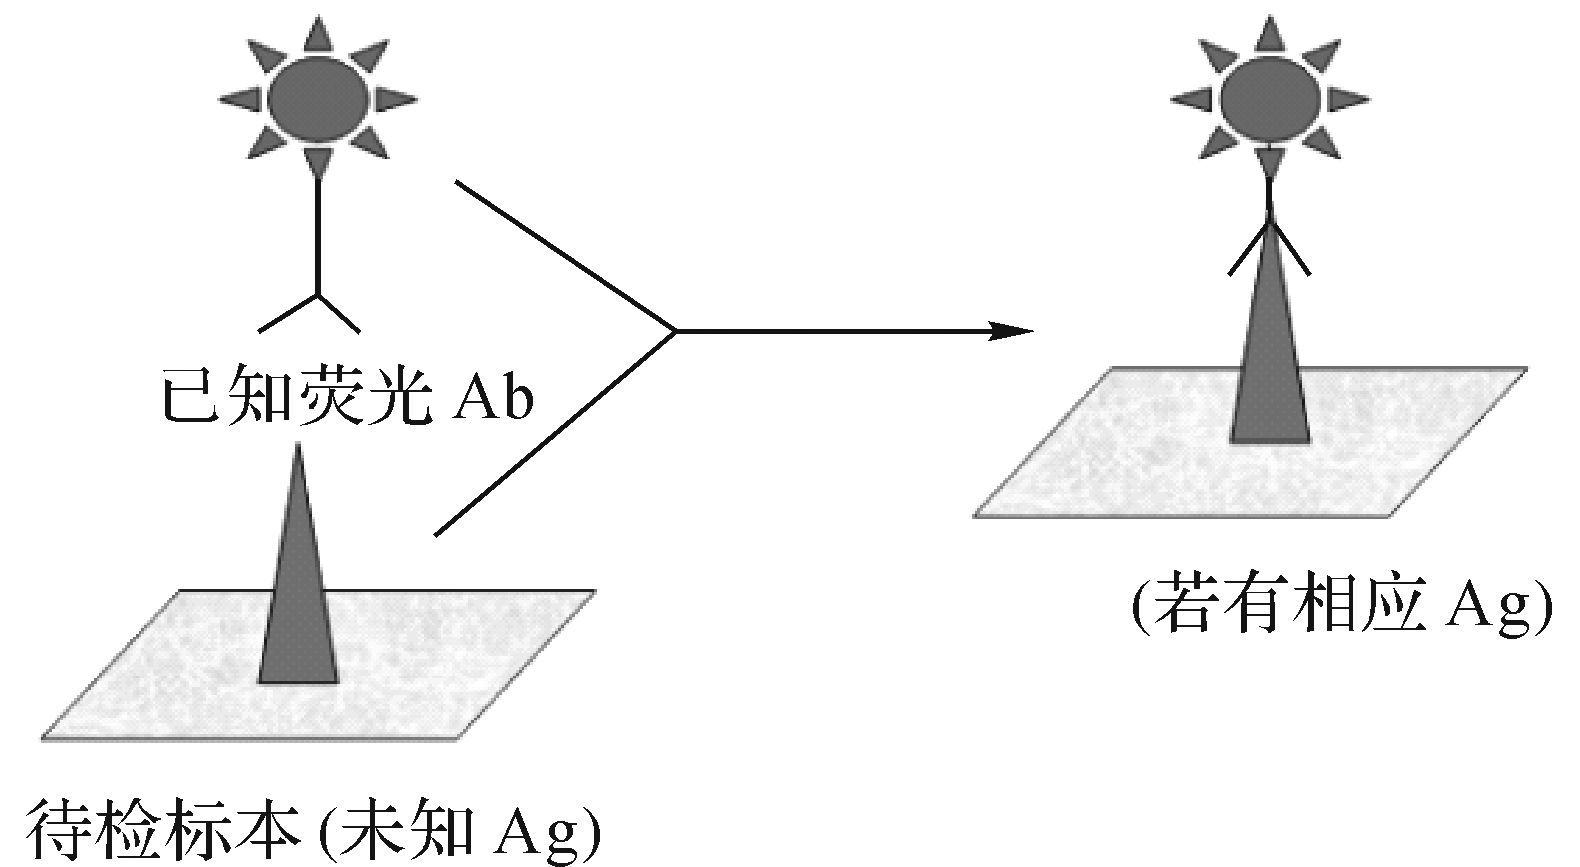
\includegraphics{./images/Image00165.jpg}
 \captionsetup{justification=centering}
 \caption{直接荧光法示意图}
 \label{fig10-13}
  \end{figure} 

2.间接法(又称荧光-抗体法)

间接法是用来检测标本中未知的抗原,或检测血清中未知抗体(图\ref{fig10-14})。

(1)检测抗原。未标记抗体+待检抗原(未知)→(冲洗)+荧光标记抗抗体→冲洗、干燥、荧光显微镜下观察。

(2)检测抗体。待检血清(未知抗体)+抗原标本(已知)→(冲洗)+荧光标记抗抗体→冲洗、干燥、荧光显微镜下观察。

优点:敏感性高,制备一种荧光标记抗抗体即可对多种抗体-抗体系统进行检测。

缺点:易出现非特异性荧光。

\begin{figure}[!htbp]
 \centering
 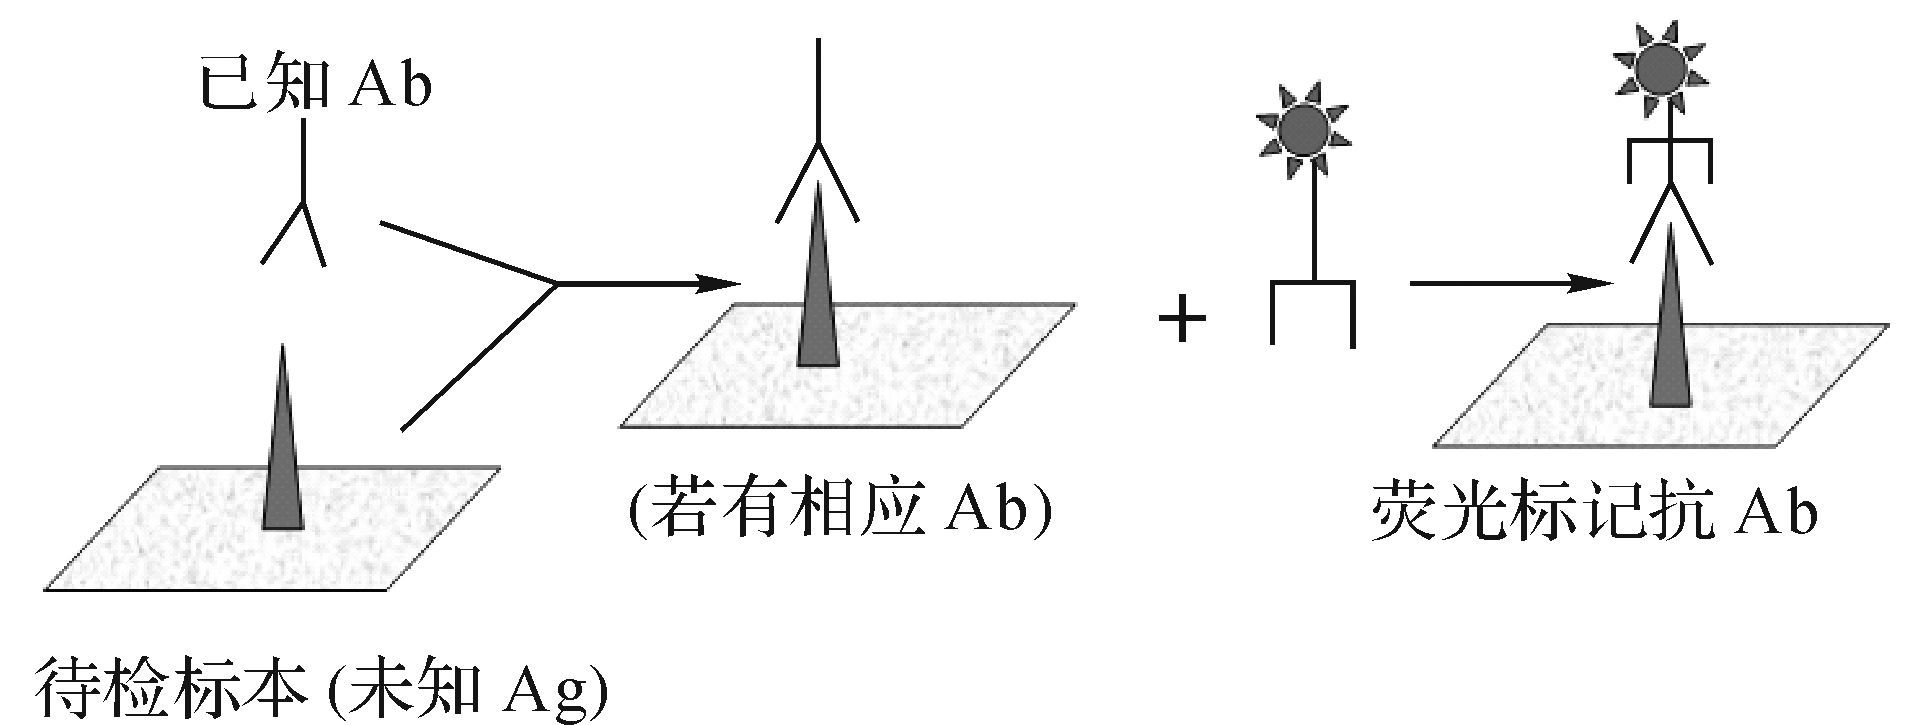
\includegraphics{./images/Image00166.jpg}
 \captionsetup{justification=centering}
 \caption{间接荧光法示意图}
 \label{fig10-14}
  \end{figure} 

3.补体法

补体法的作用原理与间接法相似,只是抗原-抗体作用后,加入新鲜豚鼠血清(补体),通过激活补体形成抗原-抗体-补体(C3b)复合物,再用荧光素标记的抗C3b抗体染色,使上述复合物发出荧光(图\ref{fig10-15})。

\begin{figure}[!htbp]
 \centering
 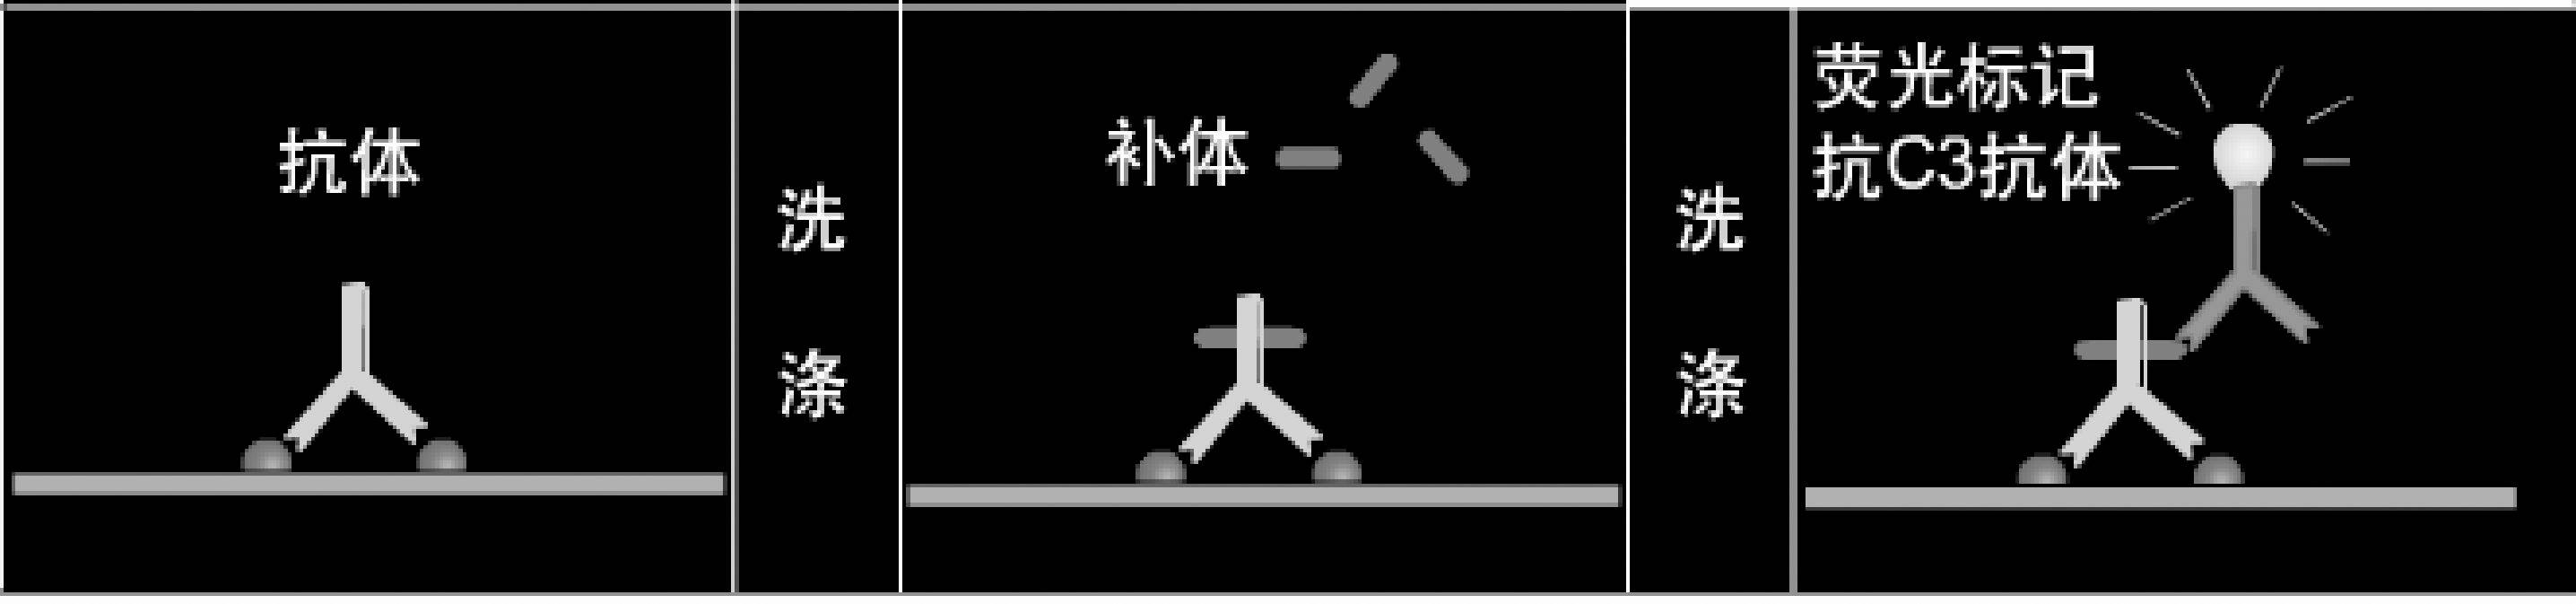
\includegraphics[width=.6\textwidth]{./images/Image00167.jpg}
 \captionsetup{justification=centering}
 \caption{补体法示意图}
 \label{fig10-15}
  \end{figure} 

(二)酶免疫测定(enzyme immunoassay,EIA)

将抗原-抗体反应的特异性与酶催化作用的高效性相结合,借助酶作用于底物的显色反应判定结果,用酶标测定仪做定性或定量分析。优点:敏感性高,特异性强,可定性、定量。

标记酶:

(1)辣根过氧化物酶(HRP)

底物:邻苯二胺(OPD)(橙色)、3,3'二氨基联苯胺(DAB)(黄褐色)。

(2)碱性磷酸酶

底物:对硝基苯磷酸盐(黄色)。

1.酶联免疫吸附试验(enzyme linked immunosorbent assay,ELISA)

酶联免疫吸附试验是利用抗原或抗体能非特异性吸附于聚苯乙烯等固相载体表面的特性,使抗原-抗体反应在固相载体表面进行的一种免疫酶技术。

(1)间接法

间接法是用已知抗原检测未知抗体的一种检测方法。用已知抗原包被固相,加入待检血清标本,再加酶标记的二抗,加底物观察显色反应(图\ref{fig10-16})。

\begin{figure}[!htbp]
 \centering
 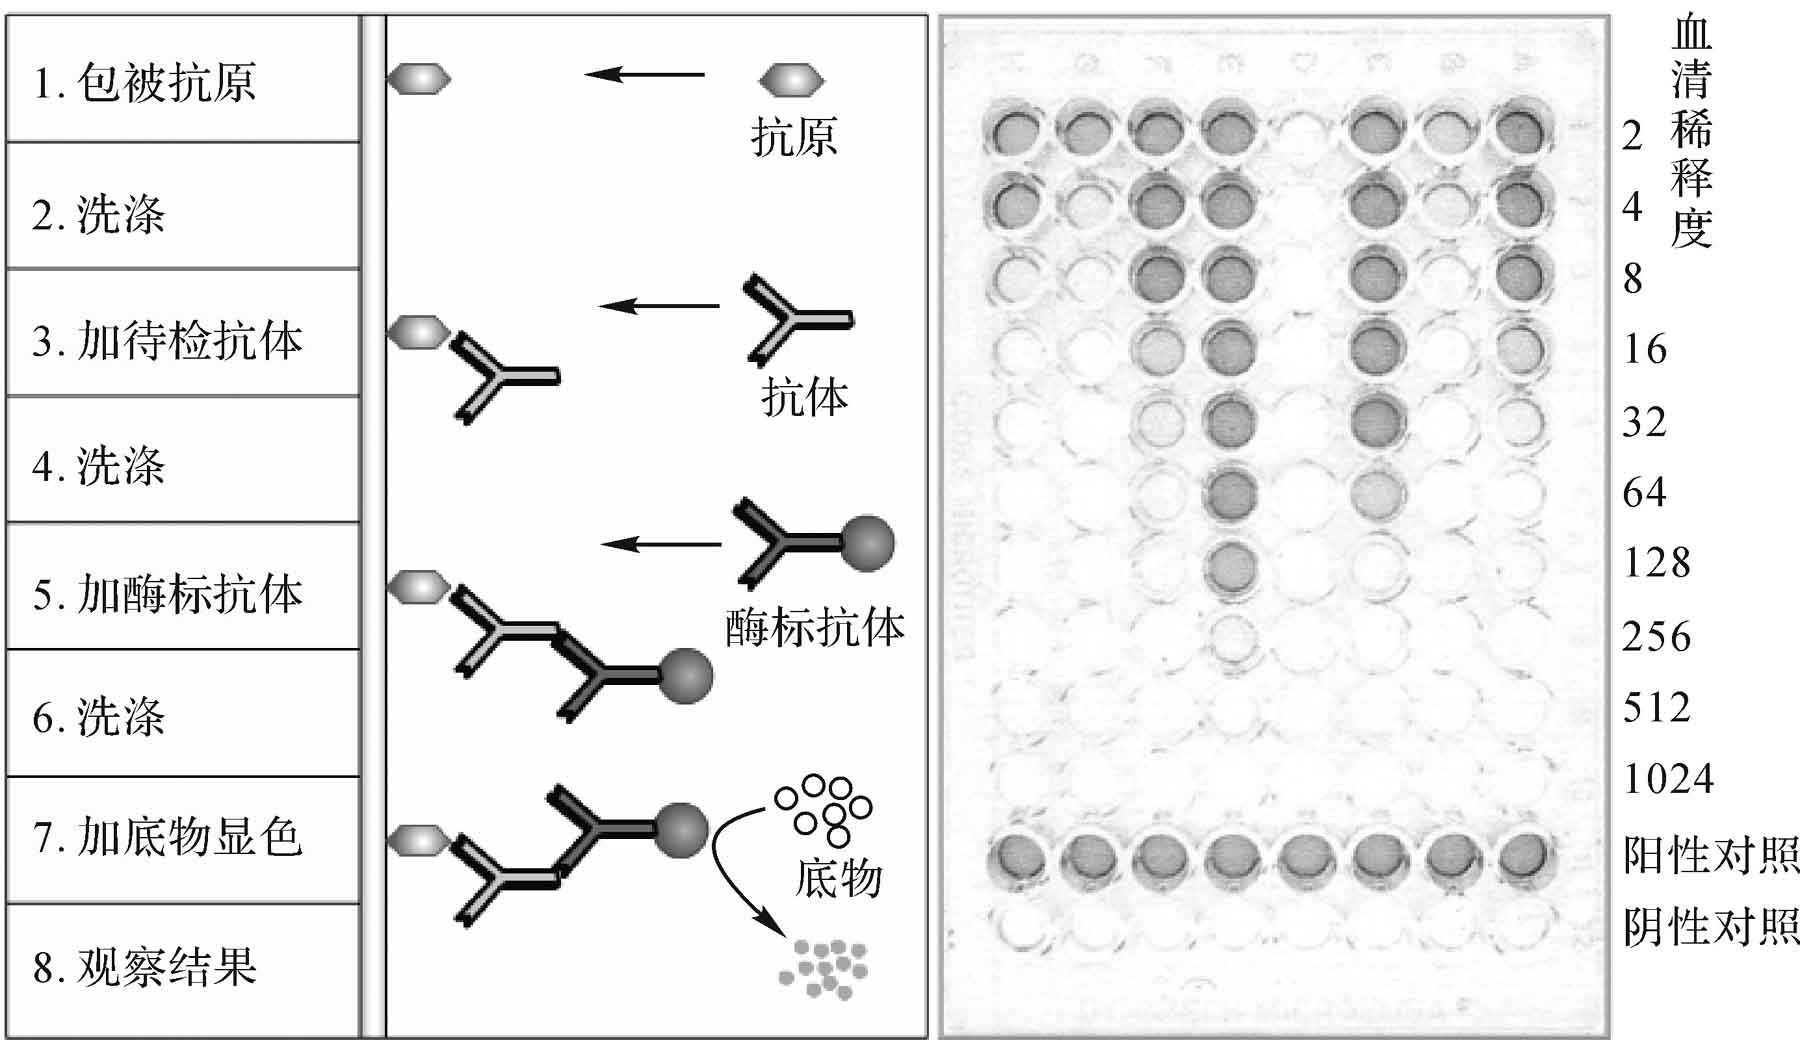
\includegraphics[width=.6\textwidth]{./images/Image00168.jpg}
 \captionsetup{justification=centering}
 \caption{ELISA间接法示意图}
 \label{fig10-16}
  \end{figure} 

(2)双抗体夹心法

双抗体夹心法是用已知抗体检测未知抗原的一种检测方法。将已知抗体包被固相载体,加入的待检标本若含有相应抗原,即与固相表面的抗体结合,洗涤去除未结合成分,加入该抗原特异的酶标记抗体,洗去未结合的酶标记抗体,加底物后显色。若标本中无相应抗原,固相表面无抗原结合,加入的酶标记抗体不能结合于固相并可被洗涤去除,加入底物则无显色反应(图\ref{fig10-17})。

\begin{figure}[!htbp]
 \centering
 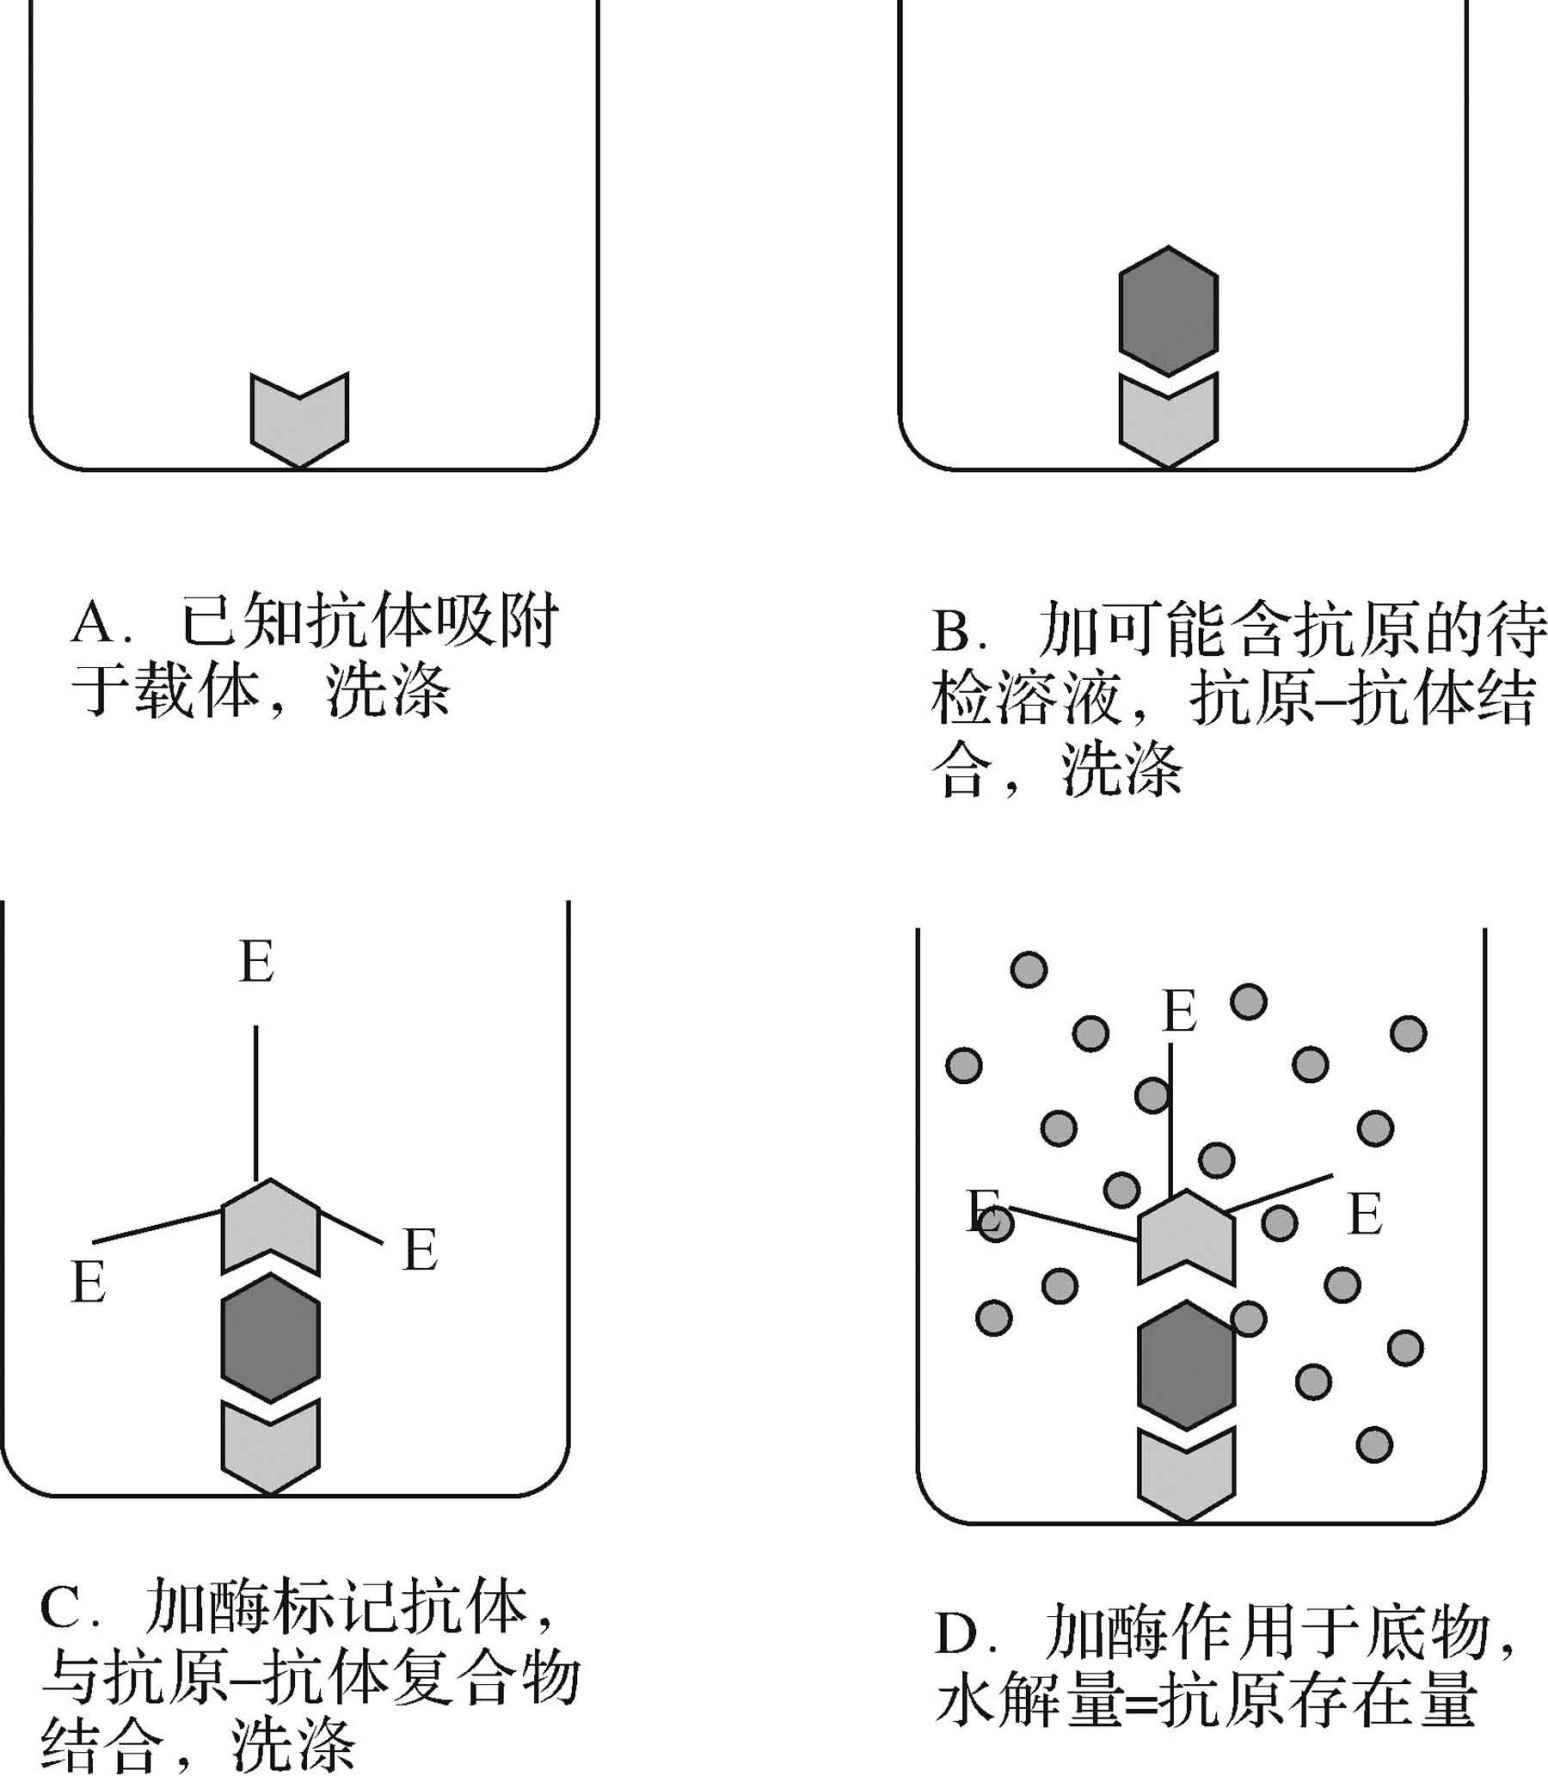
\includegraphics[width=.5\textwidth]{./images/Image00169.jpg}
 \captionsetup{justification=centering}
 \caption{双抗体夹心法示意图}
 \label{fig10-17}
  \end{figure} 

(3)酶联免疫斑点试验

酶联免疫斑点试验(ELISPOT)有两种方法:

①用已知抗原检测分泌性特异性抗体的B细胞:用已知抗原包被固相载体,B细胞分泌的抗体与之结合,加入酶标记的抗Ig抗体,通过底物显色反应可检测B细胞分泌的特异性抗体。

②用抗细胞因子抗体检测细胞分泌的细胞因子:用抗细胞因子抗体包被固相载体,加入不同来源的细胞,细胞所分泌的细胞因子与包被抗体结合,再加入酶标记的抗细胞因子抗体,通过显色反应测定结合在固相载体上的细胞因子(定性或半定量),并可在光镜下观察分泌细胞因子的细胞(图\ref{fig10-18})。

\begin{figure}[!htbp]
 \centering
 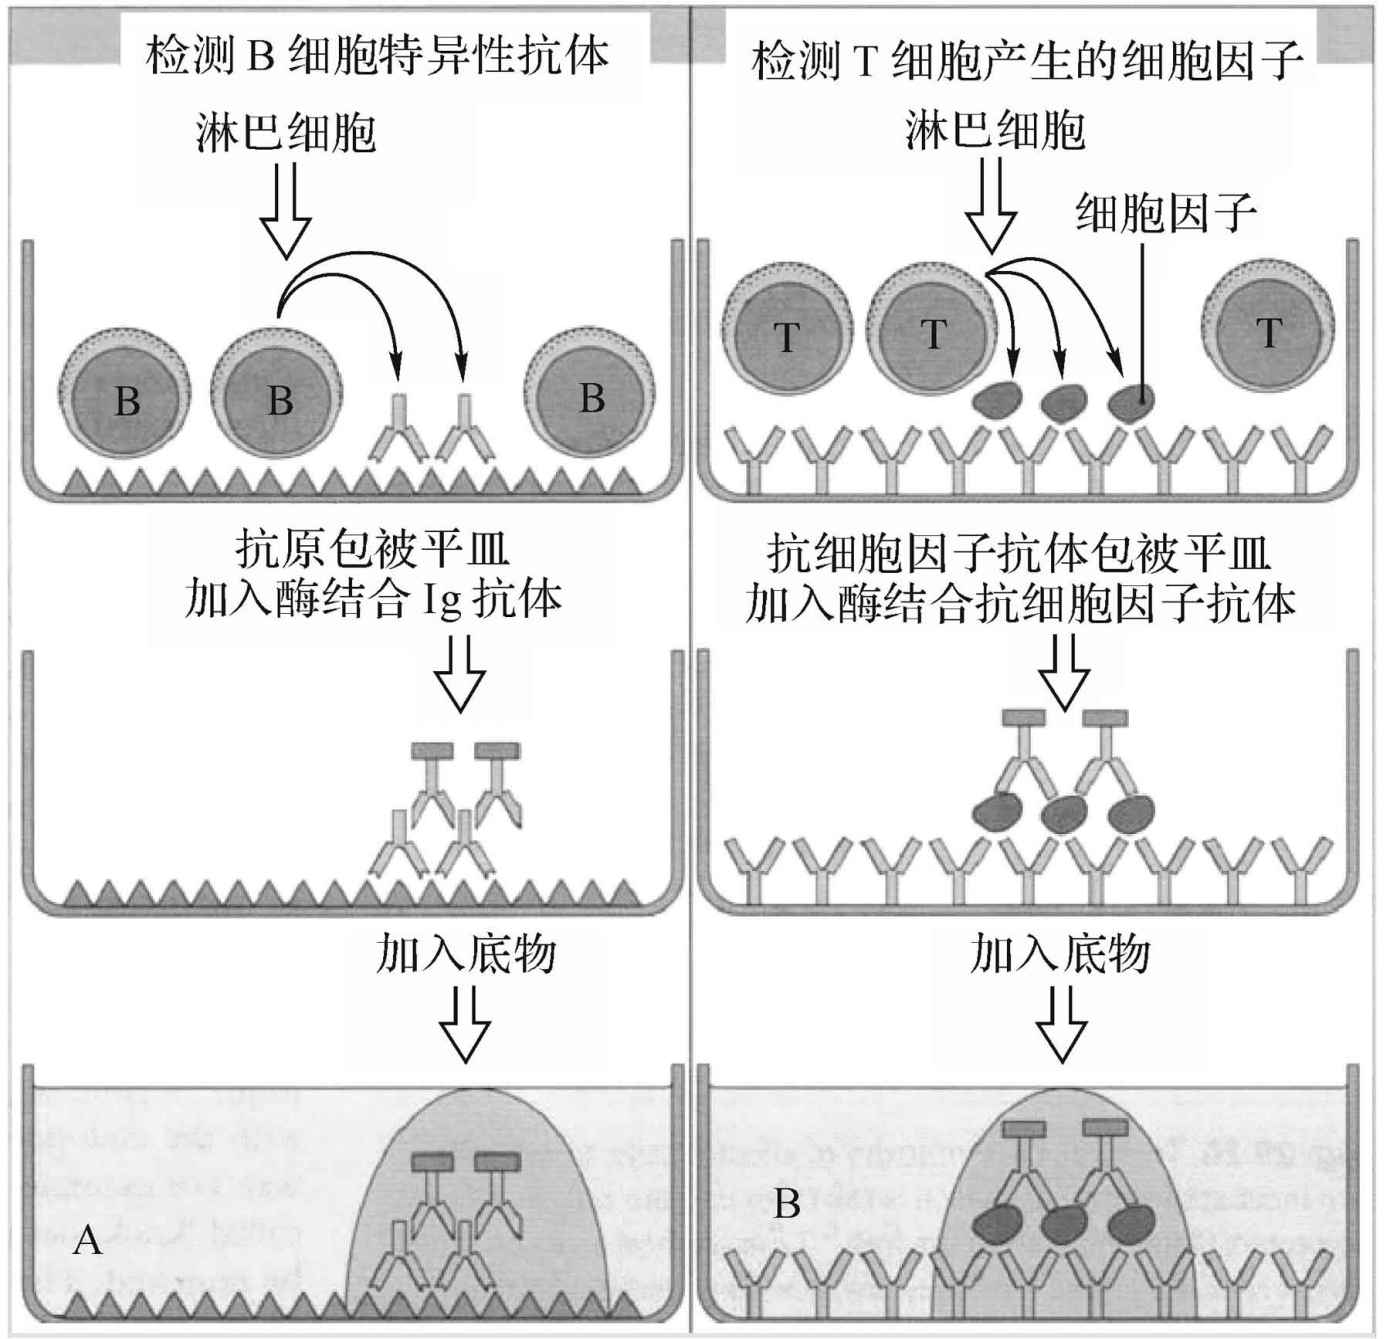
\includegraphics[width=.5\textwidth]{./images/Image00170.jpg}
 \captionsetup{justification=centering}
 \caption{酶联免疫斑点试验示意图}
 \label{fig10-18}
  \end{figure} 

(4)生物素-亲合素法

生物素(biotin)又称维生素H,是从卵黄和肝中提取的一种小分子物质(分子量244.31kD);亲合素(avidin)又称卵白素,是从卵白中提取的一种糖蛋白(分子量68kD)。每个亲合素分子有生物素结合的4个位点,二者可牢固结合成不可逆的复合物。生物素-亲合素的应用大致有三种方法(图\ref{fig10-19})。

①标记亲合素-生物素法(labelled avidin-biotin
method,LAB法):将亲合素与标记物(HRP)结合,一个亲合素可结合多个HRP;将生物素与抗体(一抗与二抗)结合,一个抗体分子可连接多个生物素分子,抗体的活性不受影响。细胞的抗原(或通过一抗)先与生物素化的抗体结合,继而将标记亲合素结合在抗体的生物素上,如此多层放大提高了检测抗原的敏感性。

\begin{figure}[!htbp]
 \centering
 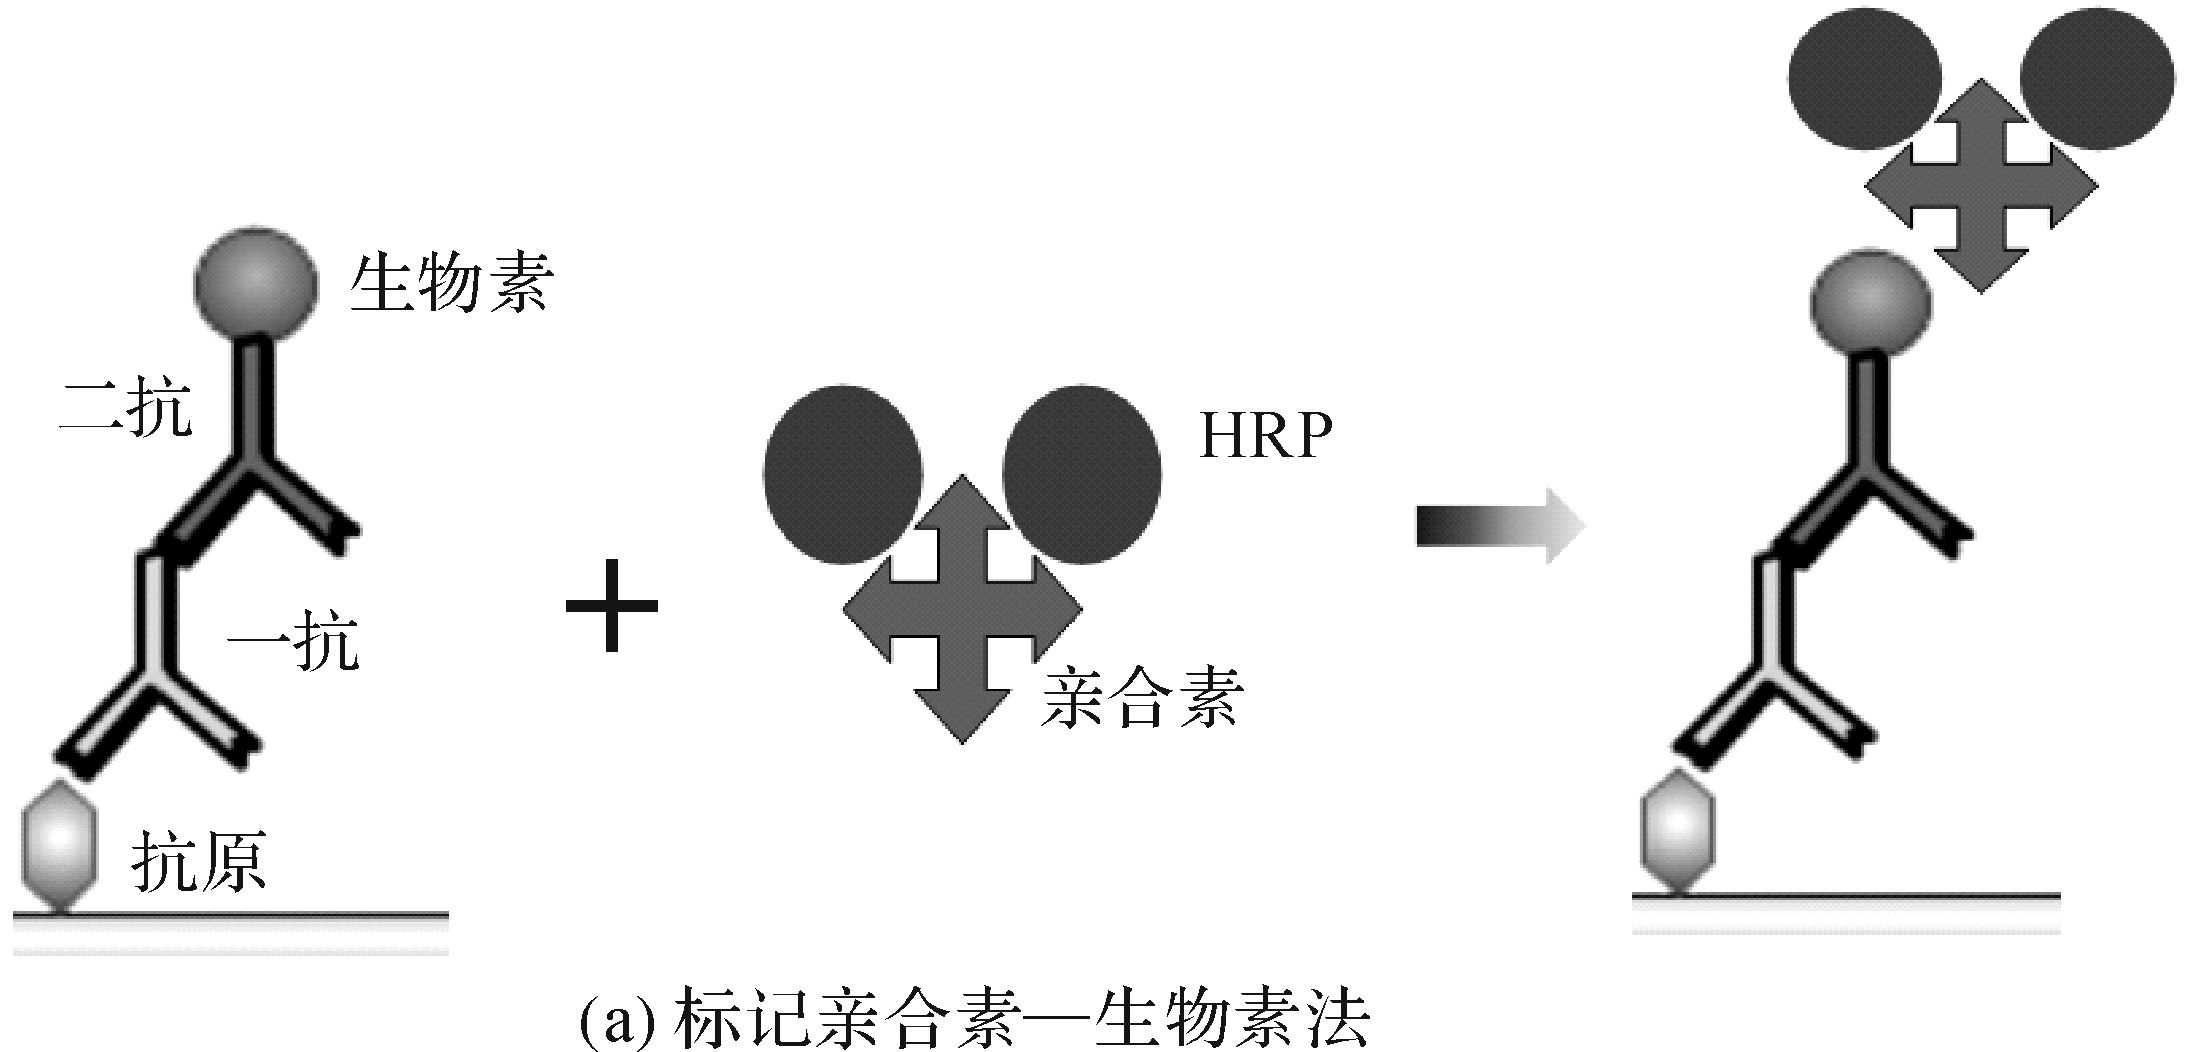
\includegraphics[width=.6\textwidth]{./images/Image00171.jpg}
 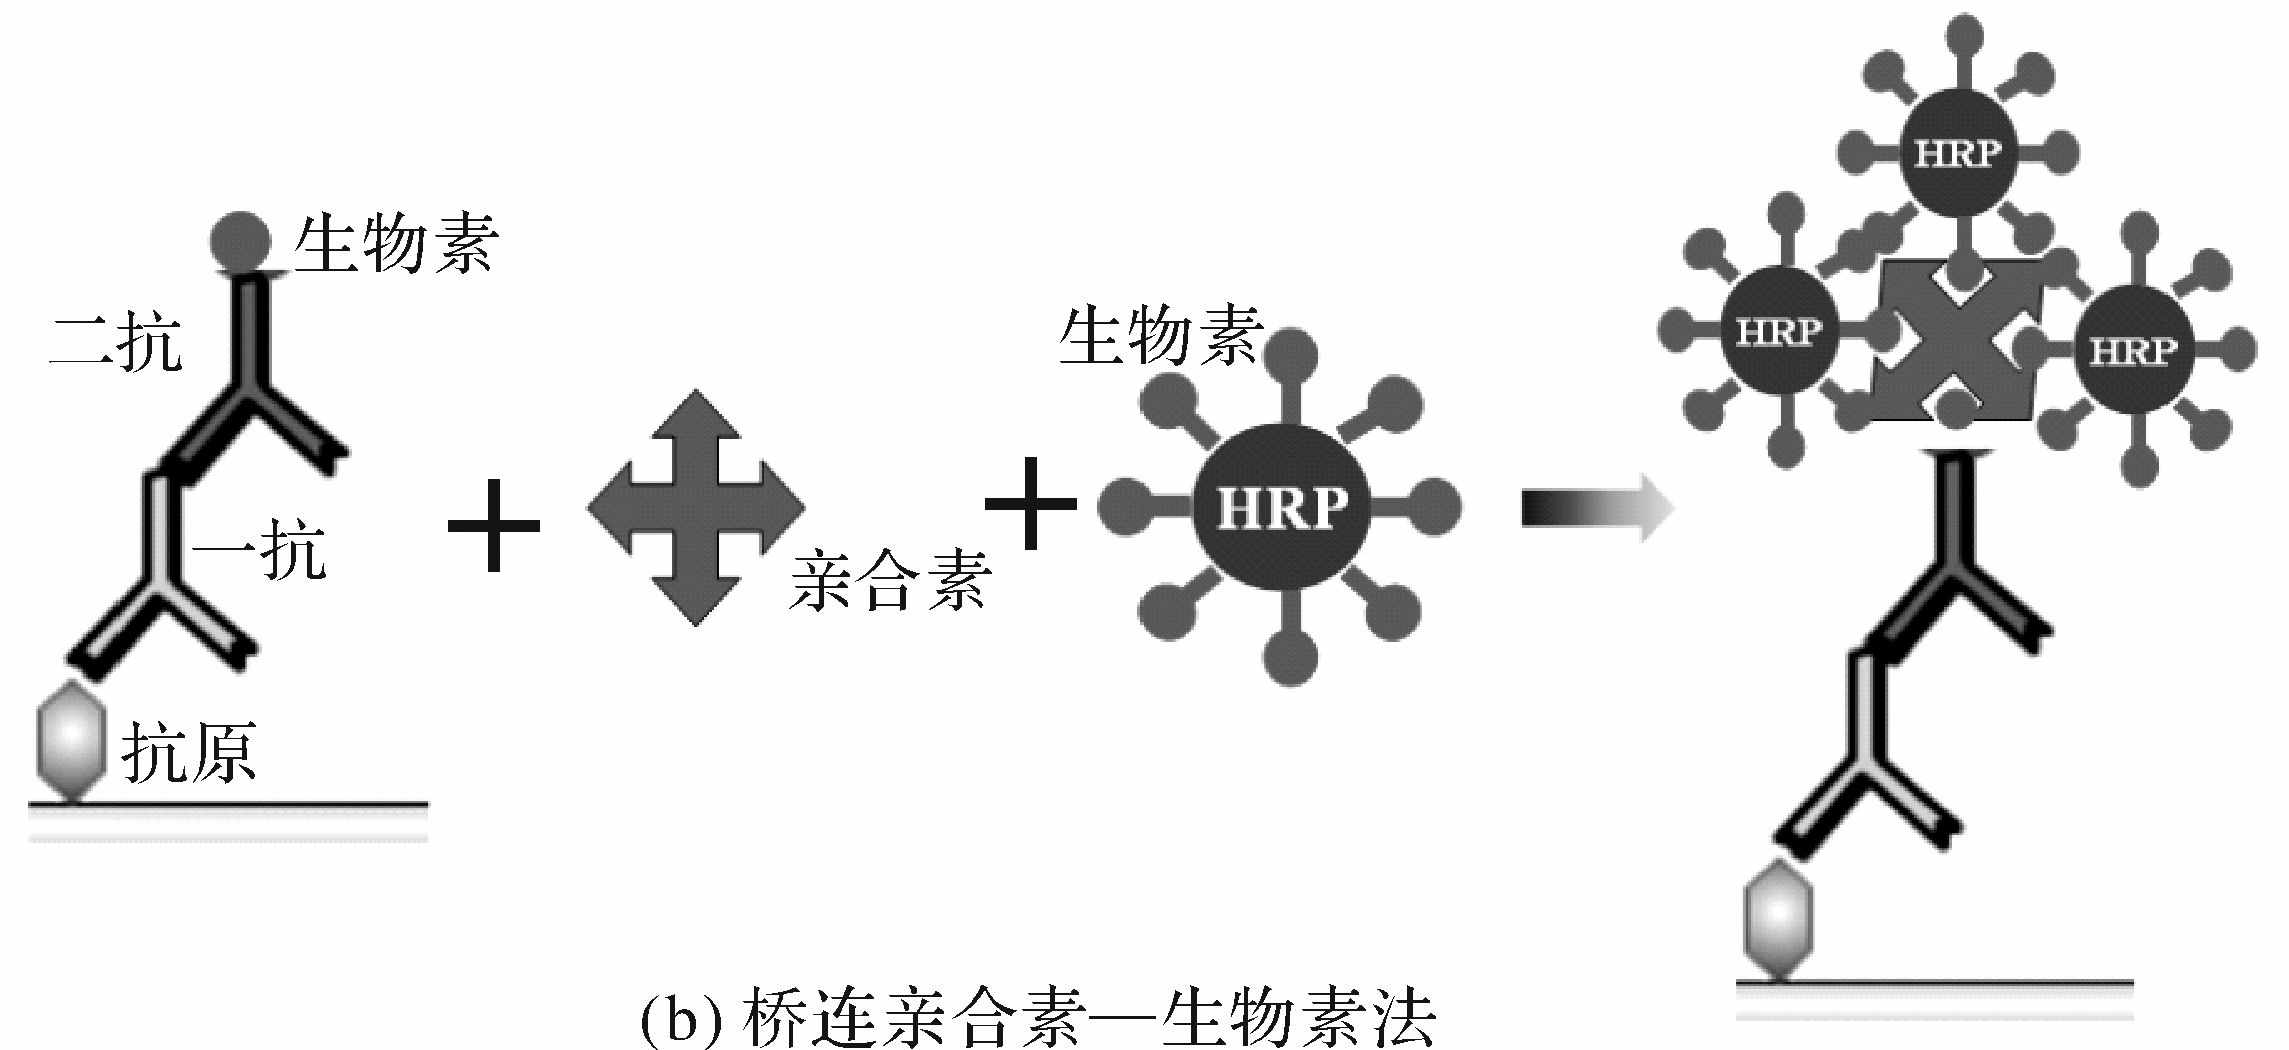
\includegraphics[width=.6\textwidth]{./images/Image00172.jpg}
 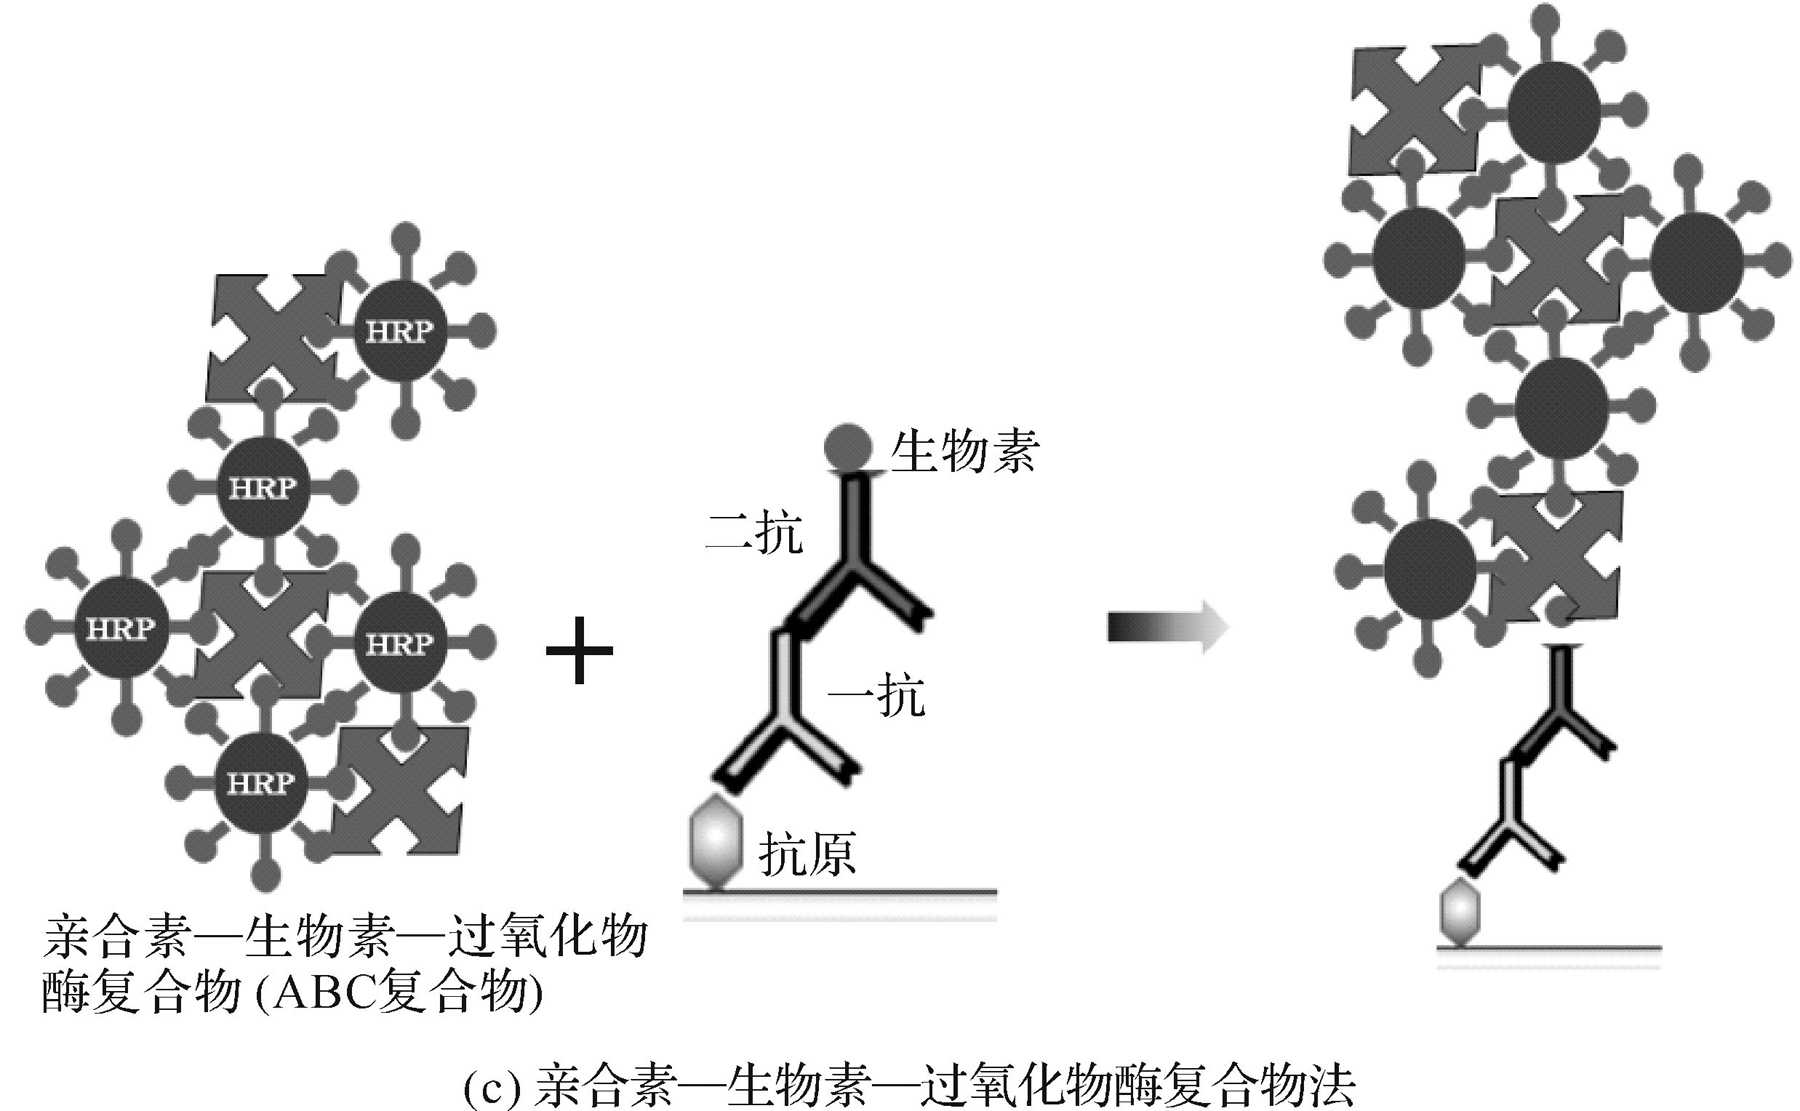
\includegraphics[width=.6\textwidth]{./images/Image00173.jpg}
 \captionsetup{justification=centering}
 \caption{生物素-亲合素法示意图}
 \label{fig10-19}
  \end{figure} 

②桥连亲合素-生物素法(bridged avidin-biotin
method,BAB法):先使抗原与生物素化的抗体结合,再以游离亲合素将生物素化的抗体与酶标生物素搭桥连接,也达到多层放大效果。

③亲合素-生物素-过氧化物酶复合物法(avidin-biotin-peroxidase complex
method,ABC法):此法是前两种方法的改进,即先按一定比例将亲合素与酶标生物素结合在一起,形成亲合素-生物素-过氧化物酶复合物(ABC复合物),标本中的抗原先后与一抗、生物素化二抗、ABC复合物结合,最终形成晶格样结构的复合体,其中聚合了大量酶分子,从而大大提高了检测抗原的灵敏度。

2.免疫组化技术

免疫组化技术(immunohitochemistry
techenique)是应用免疫学基本原理------抗原抗体反应,即抗原与抗体特异性结合的原理,通过化学反应使标记抗体的显色剂
(荧光素、酶、金属离子、同位素)
显色来确定组织细胞内抗原(多肽和蛋白质),对其进行定位、定性及定量的研究,称为免疫组织化学技术(immunohistochemistry)或免疫细胞化学技术(immunocytochemistry)。

众所周知,抗体与抗原之间的结合具有高度的特异性。免疫组化正是利用这一特性,即先将组织或细胞中的某些化学物质提取出来,以其作为抗原或半抗原去免疫小鼠等实验动物,制备特异性抗体,再用这种抗体(第一抗体)作为抗原去免疫动物制备第二抗体,并用某种酶(常用辣根过氧化物酶)或生物素等处理后再与前述抗原成分结合,将抗原放大,由于抗体与抗原结合后形成的免疫复合物是无色的,因此,还必须借助于组织化学方法将抗原抗体反应部位显示出来(常用显色剂DAB显示为棕黄色颗粒)。通过抗原抗体反应及呈色反应,显示细胞或组织中的化学成分,在显微镜下可清晰看见细胞内发生的抗原抗体反应产物,从而能够在细胞或组织原位确定某些化学成分的分布、含量。组织或细胞中凡是能作为抗原或半抗原的物质,如蛋白质、多肽、氨基酸、多糖、磷脂、受体、酶、激素、核酸及病原体等都可用相应的特异性抗体进行检测。

免疫组织化学技术按照标记物的种类可分为免疫荧光法、免疫酶法、免疫铁蛋白法、免疫金法及放射免疫自影法等(图\ref{fig10-20})。

\begin{figure}[!htbp]
 \centering
 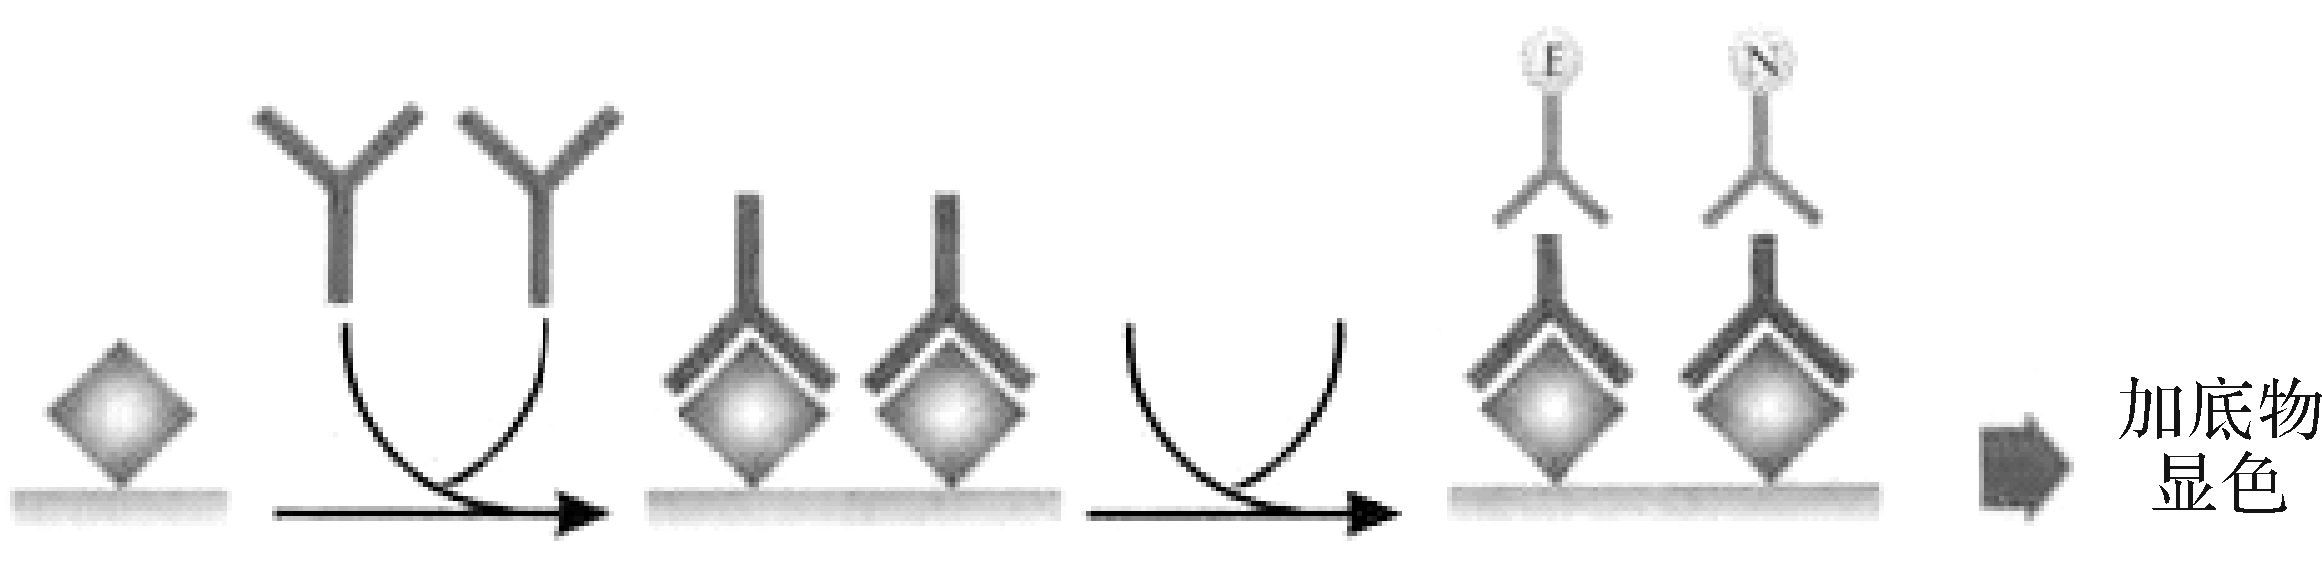
\includegraphics{./images/Image00174.jpg}
 \captionsetup{justification=centering}
 \caption{双标记免疫组化染色技术示意图}
 \label{fig10-20}
  \end{figure} 

(三)放射免疫测定

放射免疫测定(radioimmunoassay,RIA)是将放射性同位素分析的高度灵敏性与抗原-抗体反应的高度特异性有效结合而建立的一种检测技术。

同位素:\textsuperscript{131} I、\textsuperscript{125}
I、\textsuperscript{3} H、\textsuperscript{14} C、\textsuperscript{32}
P等。

特点:灵敏度高,能测出ng/ml(ug/L),甚至pg/ml(ng/L)水平的微量物质,试验快速、准确,可规格化,重复性好。

缺点:放射性同位素有一定的危害性,且易污染环境,因此其应用受到一定限制。

方法:(1)液相放射免疫测定、(2)固相放射免疫测定。

(四)化学发光免疫分析

将发光物质(如吖啶酯、鲁米诺等)标记抗原或抗体,发光物质在反应剂(如过氧化阴离子)激发下生成激发态中间体,当回复至稳定的基态时发射光子,通过自动发光分析仪测定光子产量,可反映待检样品中抗体或抗原含量(图\ref{fig10-21})。

\begin{figure}[!htbp]
 \centering
 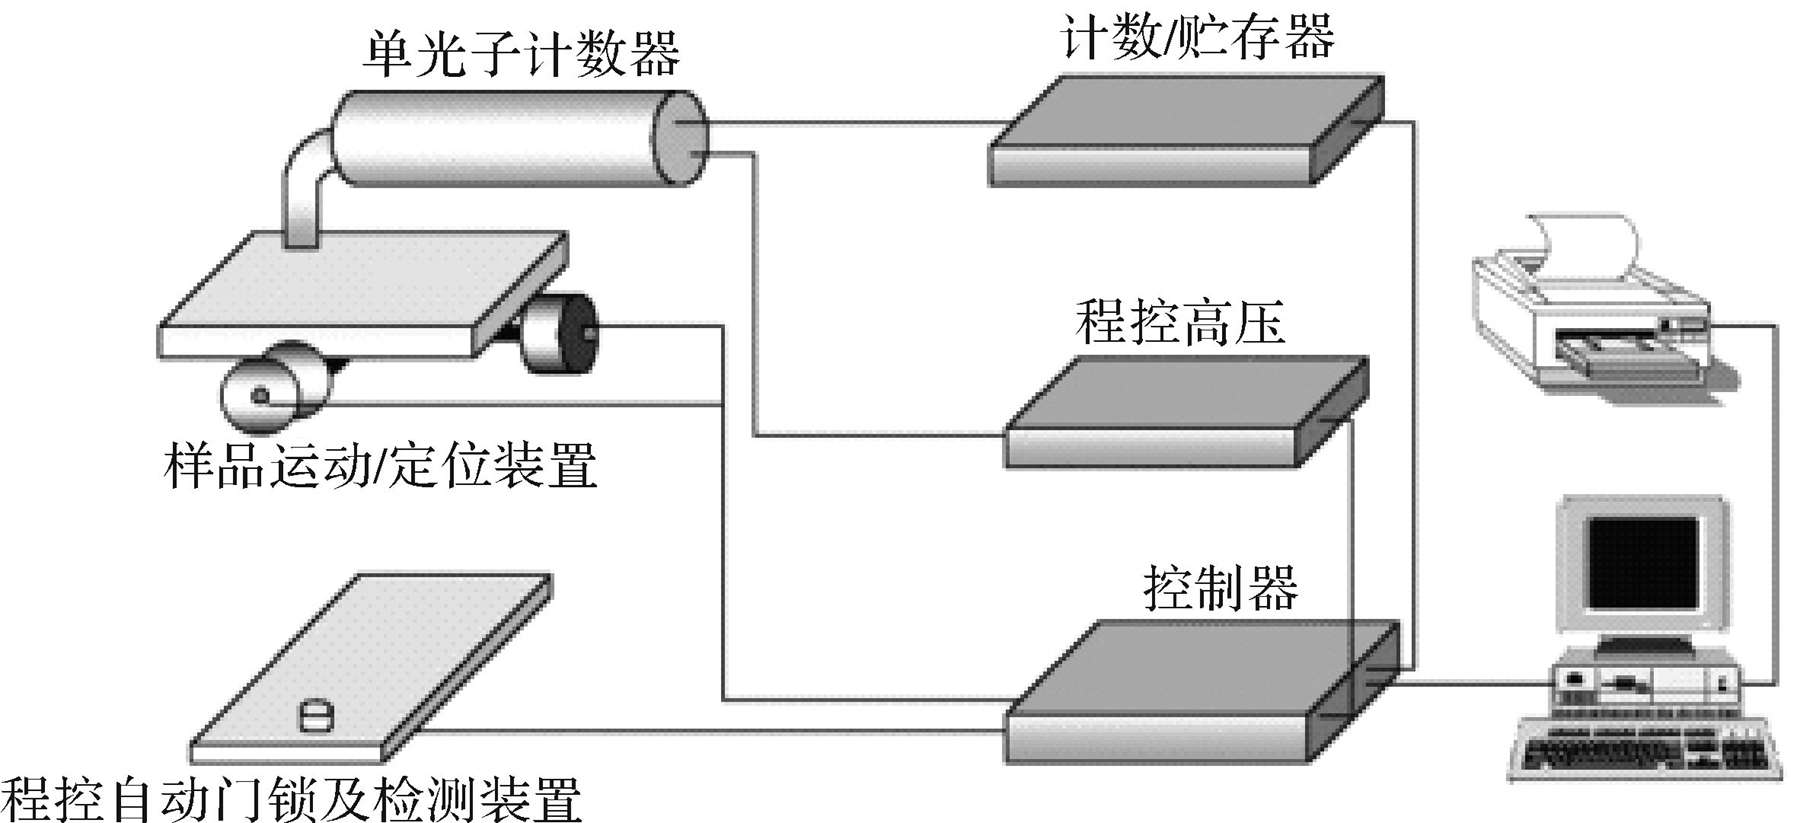
\includegraphics{./images/Image00175.jpg}
 \captionsetup{justification=centering}
 \caption{化学发光免疫分析}
 \label{fig10-21}
  \end{figure} 

(五)免疫印迹法

免疫印迹法(immunoblot)
又称Western印迹法,其结合凝胶电泳与固相免疫技术,将借助电泳所区分的蛋白质转移至固相载体,再应用酶免疫、放射免疫等技术进行检测。本方法包括5个步骤:

(1)固定:蛋白质进行聚丙烯酰胺凝胶电泳(P抗原E)并从胶上转移到硝酸纤维素膜上。

(2)封闭:保持膜上没有特殊抗体结合的场所,使场所处于饱和状态,用以保护特异性抗体结合到膜上,并与蛋白质反应。

(3)初级抗体(第一抗体)是特异性的。

(4)第二抗体或配体试剂对于初级抗体是特异性结合并作为指示物。

(5)适当保温后的酶标记蛋白质区带,产生可见的、不溶解状态的颜色反应。

该法能对分子大小不同的蛋白质进行分离并确定其分子量,常用于检测多种病毒抗体或抗原。

(六)免疫金技术

免疫金技术是一种以胶体金作为标记物的免疫标记技术。胶体金是由金盐被还原成原金后形成的金颗粒悬液,颗粒大小多在1~100nm。

胶体金的光散射性与溶胶颗粒的大小密切相关,一旦颗粒大小发生变化,光散射也随之发生变异,产生肉眼可见的显著的颜色变化。小:2~5nm,橙黄色。中:10~20nm,酒红色。大:30~80nm,紫红色。

(七)免疫比浊

免疫比浊(immunonephelometry)
是在一定量抗体中分别加入递增量的抗原,经一定时间形成免疫复合物,液体混浊。用浊度计测量反应体系的浊度,可绘制标准曲线并依据浊度推算样品中抗原含量。

\section{检测淋巴细胞及其功能的体外试验}


\subsection{免疫细胞及其亚类分离、鉴定和检测}

(一)外周血单个核细胞的分离

体外检测淋巴细胞,首先需制备外周血单个核细胞(PBMC),常用的方法是葡聚糖-泛影葡胺(又称淋巴细胞分离液)密度梯度离心法。红细胞和多形核白细胞的比重(约1.092)大于单个核细胞(约1.075),将抗凝血叠加于比重为1.077的分离液液面上,可通过低速离心将不同比重的细胞分层:红细胞沉于管底;多形核白细胞密集布于红细胞层与分离液之间;血小板悬浮于血浆中;单个核细胞则密集于血浆层与分离液界面。该法分离淋巴细胞的纯度可达95\%。若需进一步纯化淋巴细胞,可将单个核细胞铺于培养皿上,由于单核细胞易与玻璃黏附而滞留于平皿表面,未吸附的细胞即主要是淋巴细胞(图\ref{fig10-22})。

(二)淋巴细胞亚群的分离

淋巴细胞为不均一的群体,可借助其表面标志及功能差异而分为不同的群和亚群。

1.尼龙棉分离法

将淋巴细胞悬液通过尼龙棉柱,B细胞易与尼龙棉黏附而滞留于柱上,T细胞则不黏附,借此可分离T细胞与B细胞。

  \begin{figure}[!htbp]
    \centering
    \begin{minipage}[b]{0.45\textwidth} 
        \centering
        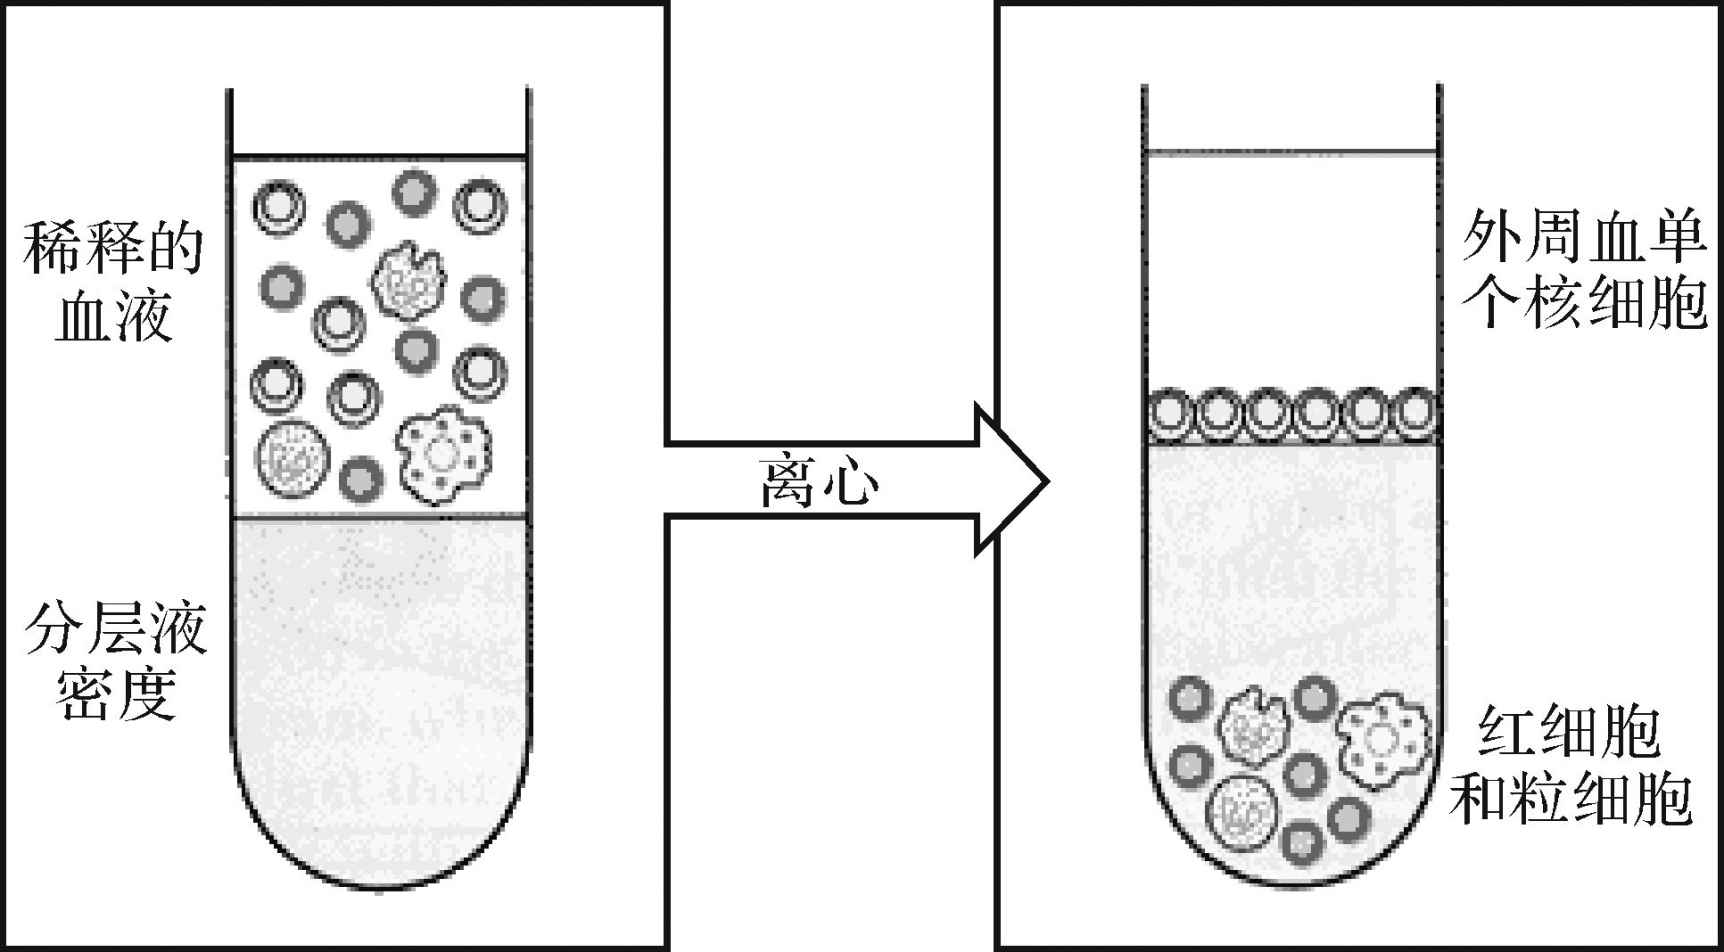
\includegraphics[height=.2\textheight]{./images/Image00176.jpg}
        \captionsetup{justification=centering}
        \caption{密度梯度离心法分离单核细胞}
        \label{fig10-22}
    \end{minipage}
%	\end{figure} 
	%\FloatBarrier
%\begin{figure}[!htbp]
%    \centering
\hspace{0.04\textwidth}%
\begin{minipage}[b]{0.45\textwidth} 
    \centering
    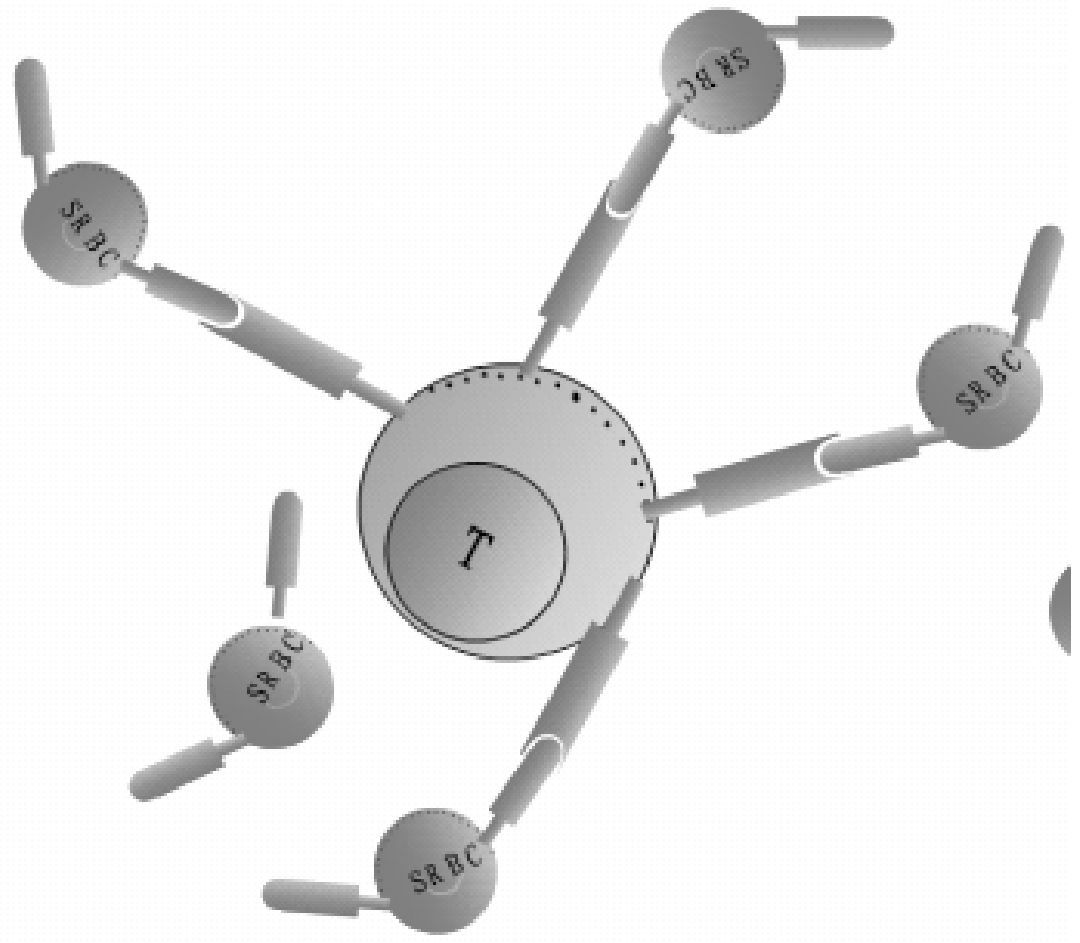
\includegraphics[height=.2\textheight]{./images/Image00177.jpg}
    \captionsetup{justification=centering}
    \caption{E花结分离法}
    \label{fig10-23}
\end{minipage}
\end{figure} 

2.E花结分离法

人成熟T细胞表面具有绵羊红细胞(SRBC)受体,能结合SRBC而形成花结(E花结试验),经密度梯度离心,花结形成细胞因比重增大而沉于管底,与其他细胞分离;用低渗法裂解花结中的SRBC,即获得纯化的T细胞(图\ref{fig10-23})。

3.洗淘法

将已知抗特定细胞表面标志的抗体包被聚苯乙烯培养板,加入淋巴细胞悬液,表达相应表面标志的细胞即结合于培养板表面,与悬液中的其他细胞分离。

4.流式细胞术(flow cytometry,FCM)

借助荧光活化细胞分类仪(fluorescence-activated cell
sorter,FACS)对细胞快速鉴定和分类,并进行多参数定量测定和综合分析的技术。样品与经多种荧光素标记的抗体反应,因荧光素发射光谱的波长不同,信号能同时被接收,故能同时分析细胞表面多个膜分子表达及其水平。该法可检测各类免疫细胞、细胞亚类及其比率。此外,借助光电效应,微滴通过电场时出现不同偏向,可分类收集所需细胞。

5.磁分离技术

将特异性抗体与磁性微粒交联,称为免疫磁珠(immune m抗原netic
bead,IMB)。IMB可与表达相应膜抗原的细胞结合,应用强磁场分离IMB及其所吸附的细胞,从而对特定的细胞进行分选,此为直接分离法;亦可用二抗包被磁性微珠,与任何已结合鼠源性一抗的细胞进行反应,从而分离细胞,此为间接分离法。

(三)T细胞及其亚群的鉴定和检测

1.E玫瑰花环形成试验

本试验可用于人T细胞的鉴定和检测。绵羊红细胞和人外周血淋巴细胞在4℃孕育1~2小时,检测花环样细胞集团数量。正常人外周血中E玫瑰花环形成细胞占淋巴细胞总数的60\%~80\%。

2.T细胞单克隆抗体对T细胞及其亚群的鉴定和检测

所用的抗体主要有:CD\textsubscript{3} McAb、CD\textsubscript{4}
McAb和CD\textsubscript{8} McAb。

方法:免疫荧光间接法。

外周血淋巴细胞,分别用小鼠抗人CD\textsubscript{3} 、CD\textsubscript{4}
、CD\textsubscript{8} McAb
(第一抗体)加荧光素标记的兔抗小鼠IgG抗体(第二抗体),在荧光显微镜下观察结合有荧光素标记抗体的细胞,亦可应用FCM自动计数荧光阳性细胞百分率(图\ref{fig10-24})。

\begin{figure}[!htbp]
 \centering
 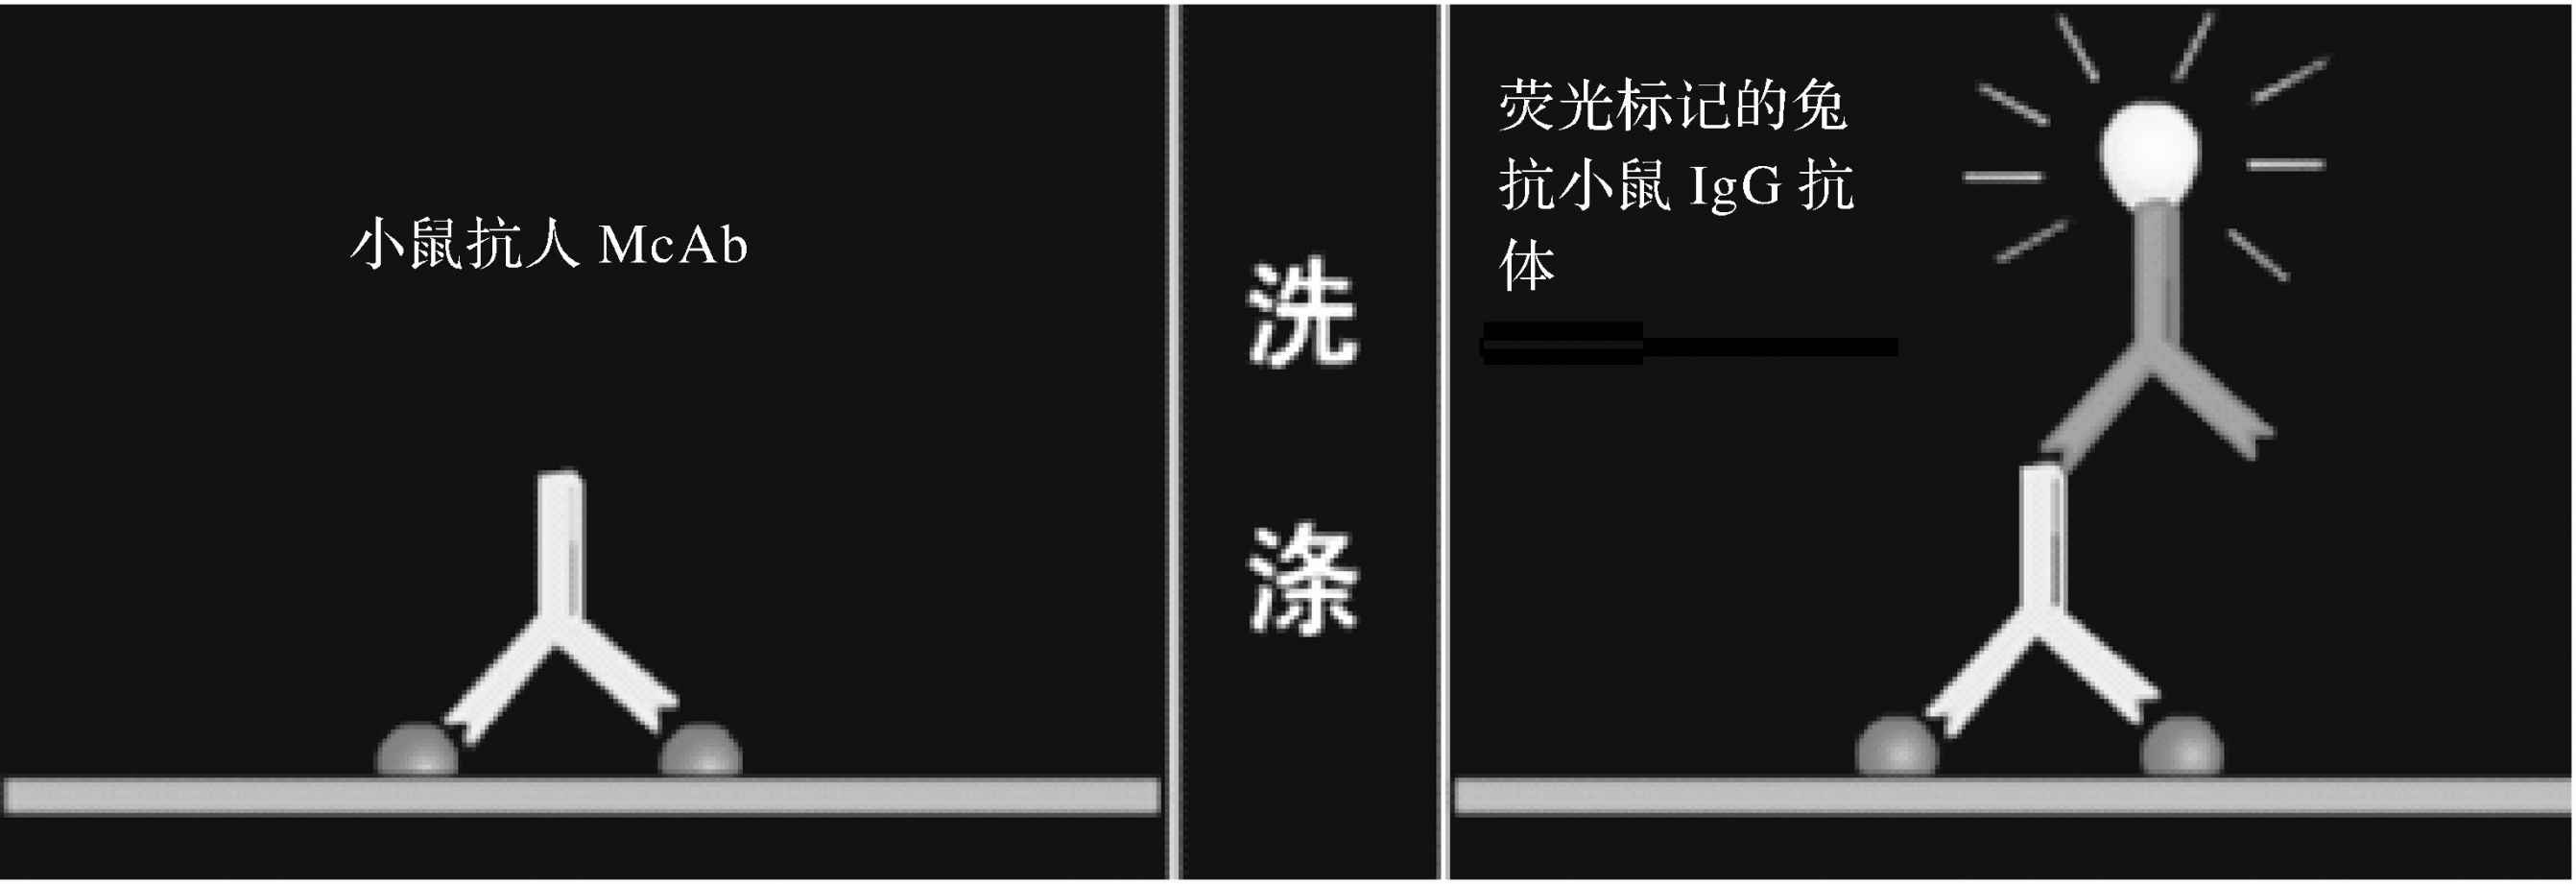
\includegraphics[width=.6\textwidth]{./images/Image00178.jpg}
 \captionsetup{justification=centering}
 \caption{免疫荧光间接法鉴定T细胞}
 \label{fig10-24}
  \end{figure} 

结果:

(1)被CD\textsubscript{3}
McAb着染荧光的细胞是总T细胞,包括:Th、Th1、Th2、Tc、Ts细胞。

(2)被CD\textsubscript{4} McAb着染荧光的细胞是Th、Th1、Th2细胞。

(3)被CD\textsubscript{8} McAb着染荧光的细胞是Tc、Ts细胞。

计数:

100~200个淋巴细胞,计算出染阳性细胞百分率:

CD\textsuperscript{+} \textsubscript{3}
T细胞占65\%~80\%。CD\textsubscript{4}
T细胞占50\%~60\%。CD\textsuperscript{+} \textsubscript{8}
T细胞占20\%~30\%。CD\textsuperscript{+} \textsubscript{4}
T细胞与CD8T细胞比值约为2∶1。

(四)B细胞鉴定和检测

\begin{figure}[!htbp]
 \centering
 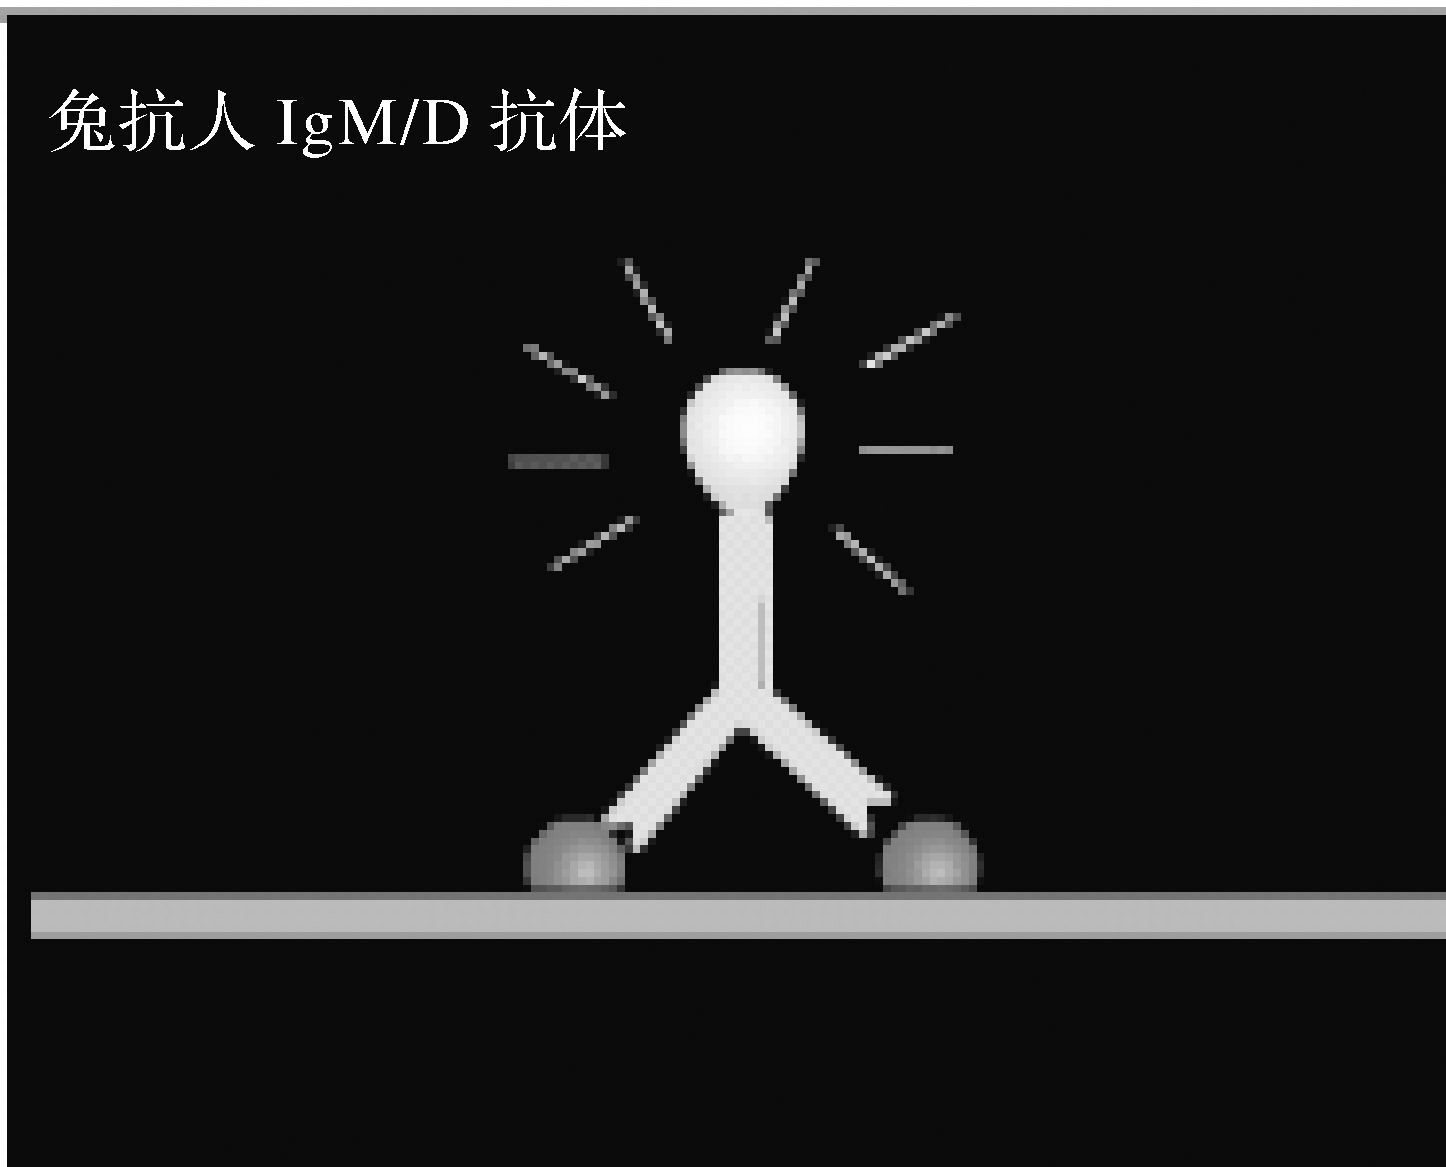
\includegraphics[width=.5\textwidth]{./images/Image00179.jpg}
 \captionsetup{justification=centering}
 \caption{免疫荧光直接法检测B细胞}
 \label{fig10-25}
  \end{figure} 

mIgM/D是B细胞表面特有的标志,通过对该种标志的检测,可对B细胞进行鉴定和检测。

方法:免疫荧光直接法。

荧光素标记的兔抗人IgM/D抗体加外周血淋巴细胞,直接免疫荧光染色、观察(图\ref{fig10-25})。着染荧光的细胞为B细胞,占淋巴细胞总数的8\%~12\%。


\subsection{淋巴细胞功能测定}

(一)T细胞功能检测

1.淋巴细胞转化试验

原理:T细胞在特异性抗原或有丝分裂原的作用下转变为淋巴母细胞(体积更大、代谢旺盛),根据其转化程度和转化率,测定机体细胞免疫功能状态。

刺激物分为两类:

(1)非特异性刺激物:如各种丝裂原(PHA、Con
A、LPS等),抗CD\textsubscript{2} 、CD\textsubscript{3}
等细胞表面标志的抗体以及某些细胞因子等;正常人T细胞转化率约为70\%。

(2)特异性刺激物:主要是特异性可溶性抗原、细胞表面抗原、结核菌素(OT或PPD)。正常人T细胞转化率为5\%~30\%。

不同刺激物可刺激不同淋巴细胞分化增殖,从而反映不同淋巴细胞亚群的功能状态。

测定方法:可采用放射性核素掺入法、比色法、荧光素标记法和形态学等方法。

(1)3H-TdR掺入法

在T细胞增殖过程中,胞内DNA、RNA合成增加,应用氚标记的胸腺嘧啶核苷(3H-TdR)可掺入细胞新合成的DNA中,所掺入放射性核素的量与细胞增殖水平成正比。借助液体闪烁仪测定样品的放射活性,可反映细胞的增殖状况。该法灵敏可靠,应用广泛,但需特殊仪器,易发生放射性污染。

(2)MTT法

MTT是一种噻唑盐,化学名3-(4,5-二甲基-2-噻唑)-2,5-二苯基溴化四唑,其掺入细胞后可作为胞内线粒体琥珀酸脱氢酶的底物,形成褐色甲臜颗粒并沉积于胞内或细胞周围,甲臢生成量与细胞增殖水平成正相关。甲臢可被盐酸异丙醇或二甲基亚砜完全溶解,借助酶标测定仪检测细胞培养物OD值,可反映细胞增殖水平。该法灵敏度不及3H-TdR掺入法,但操作简便,且无放射性污染。

(3)形态学计数法

淋巴细胞受丝裂原刺激后,转化为淋巴母细胞,其形态和结构发生明显改变,通过染色镜检,可计算出淋巴细胞转化率。

2.淋巴细胞参与的细胞毒性试验(LMC-T)

CTL、NK细胞可直接杀伤不同靶细胞(如肿瘤细胞、移植供体细胞等)。通过检测杀伤活性可用于肿瘤免疫、移植排斥反应、病毒感染等方面研究。

(1)\textsuperscript{51} Cr释放法

用Na\textsuperscript{51} \textsubscript{2} CrO\textsubscript{4}
标记靶细胞,被效应细胞杀伤的靶细胞释放\textsuperscript{51}
Cr,应用γ计数仪测定所释出的\textsuperscript{51}
Cr放射活性,可反映效应细胞的杀伤活性(图\ref{fig10-26})。

\begin{figure}[!htbp]
 \centering
 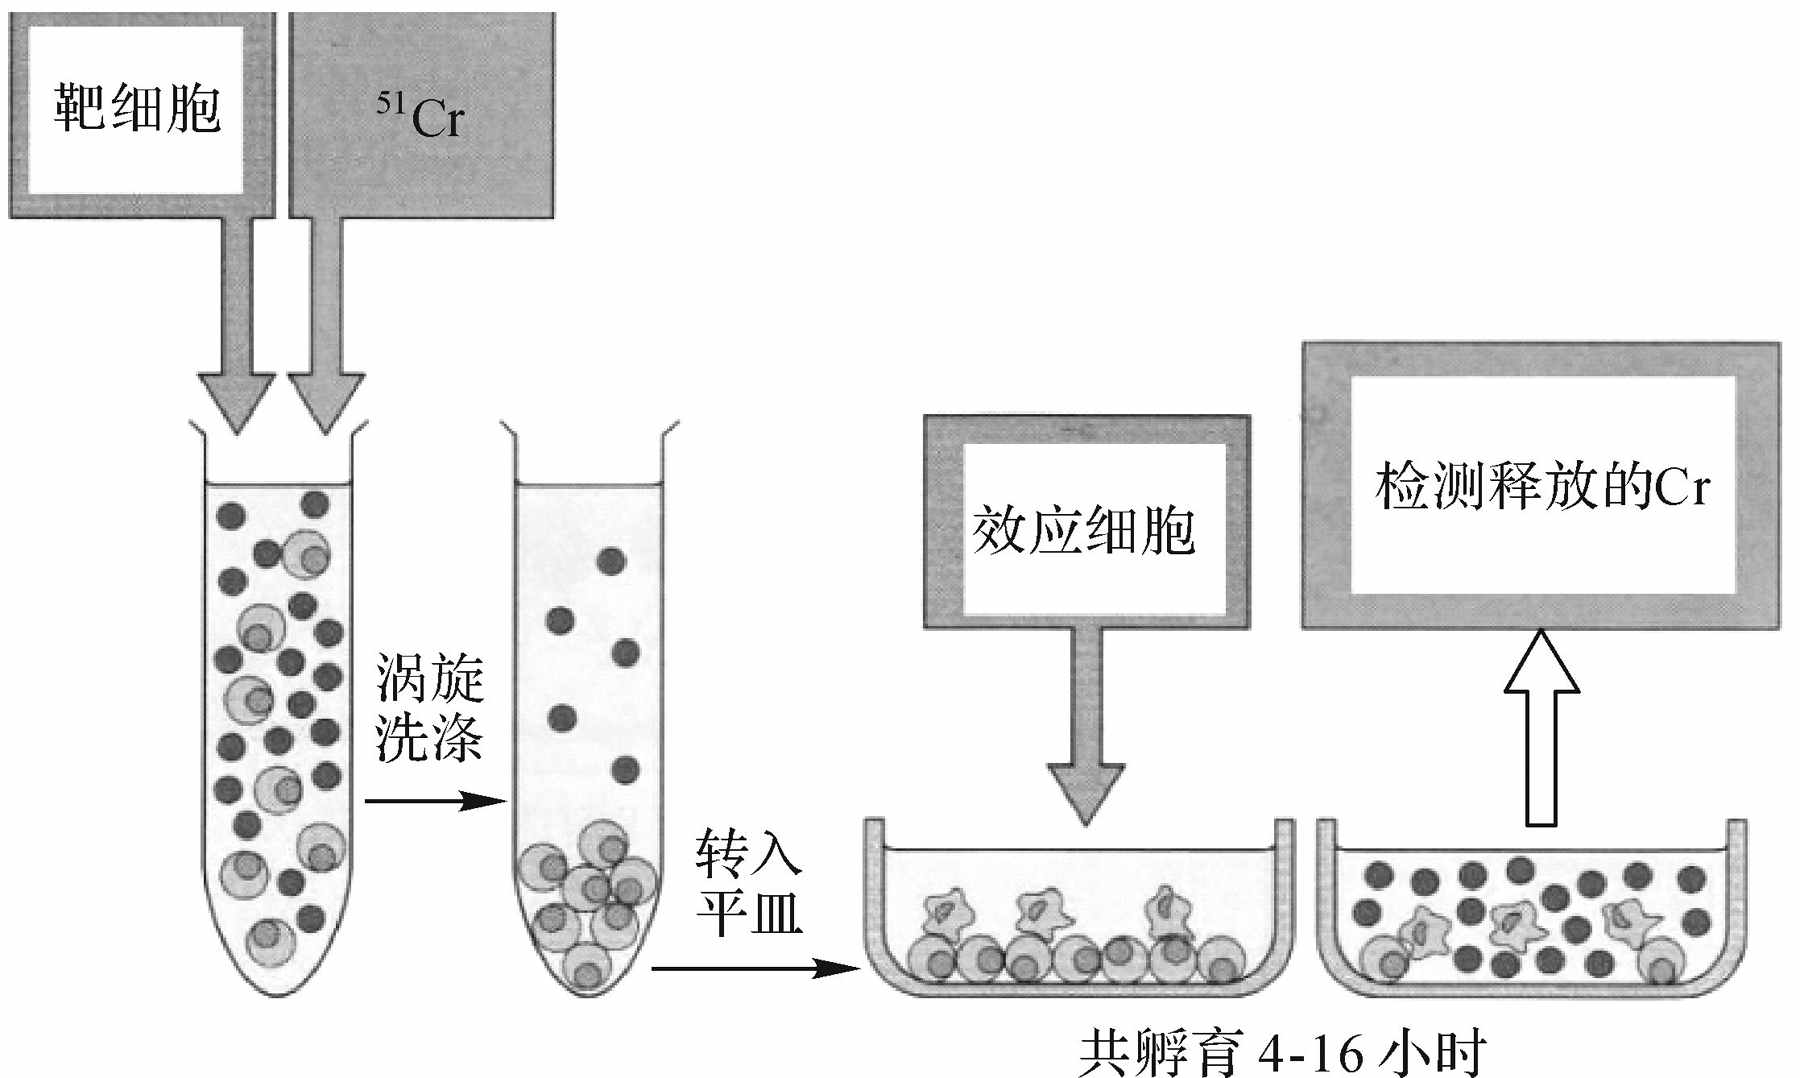
\includegraphics[width=.6\textwidth]{./images/Image00180.jpg}
 \captionsetup{justification=centering}
 \caption{Cr释放法细胞毒试验}
 \label{fig10-26}
  \end{figure} 

(2)乳酸脱氢酶(LDH)释放法

效应细胞-靶细胞进行反应并离心,借助比色法测定靶细胞膜受损后从胞内所释放出的乳酸脱氢酶活性,其水平反映效应细胞的杀伤活性。

(3)细胞凋亡检查法

效应细胞介导靶细胞凋亡时,内源性核酸水解酶将靶细胞DNA在核小体单位之间被切断,产生180~200bp(核小体单位长度)及其倍数的寡核苷酸片段,在琼脂糖电泳中呈现阶梯状DNA区带图谱,借此可反映细胞凋亡。

如需测定凋亡细胞数目及细胞类型,可在细胞培养物中加入末端脱氧核苷酸转移酶(terminal
deoxyribonucleotidyl
transferase,TdT)和生物素标记的核苷酸,TdT能在游离的DNA
3'端缺口连接标记的核苷酸,利用亲合素-生物素-酶放大系统,在DNA断裂处显色,从而指示凋亡细胞。该法所用标记核苷酸多为dUTP,故称TUNEL法(TdT
dependent dUTP-biotin nick end labelling)。

3.分泌功能测定

检测免疫细胞所分泌细胞因子和抗体水平,可反映机体免疫功能状态。

(1)细胞因子分泌细胞的测定

细胞因子分泌细胞的测定常采用反向溶血空斑试验(RHPA)和酶联免疫斑点试验(ELISPOT)。RHPA检测原理是:将分泌细胞因子的待测细胞置于经SPA包被的单层SRBC中,抗细胞因子抗体被SPA固定在SRBC表面,并与待测细胞所分泌细胞因子结合。在补体存在时,细胞因子及其抗体形成的复合物可激活补体,溶解附近的红细胞形成溶血空斑。空斑大小与细胞分泌细胞因子的量成正比。

(2)抗体形成细胞测定

抗体形成细胞测定常用溶血空斑试验和定量溶血分光光度测定法。

溶血空斑试验即测定针对SRBC表面已知抗原的抗体形成细胞数目。其原理是:抗体形成细胞分泌的Ig与SRBC表面抗原结合,在补体参与下出现溶血反应。每一空斑中央含一个抗体形成细胞,空斑数目即为抗体形成细胞数(图\ref{fig10-27})。亦可采用RHPA和ELISPOT法检测抗体分泌细胞。

定量溶血分光光度测定法原理:根据溶血空斑试验原理衍化而来。将绵羊红细胞免疫小鼠后获得的脾细胞(含抗体形成细胞)与绵羊红细胞(SRBC)及豚鼠新鲜血清(补体)按一定比例混合,37℃水浴1小时后,SRBC溶解,释放血红蛋白,离心后上清液中的血红蛋白可用分光光度计定量测定。所获上清液吸光值与抗体形成细胞(浆细胞)分泌的抗体量成正比。

\begin{figure}[!htbp]
 \centering
 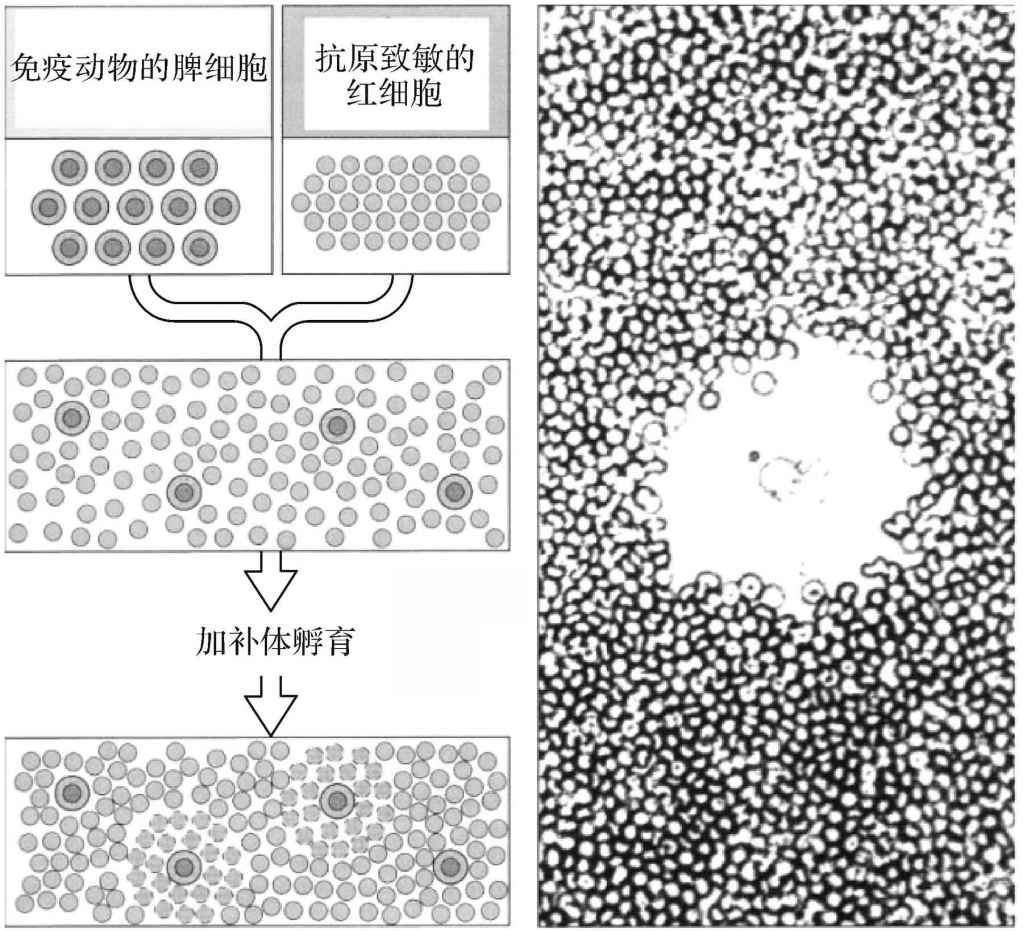
\includegraphics[width=.6\textwidth]{./images/Image00181.jpg}
 \captionsetup{justification=centering}
 \caption{溶血空斑试验}
 \label{fig10-27}
  \end{figure} 

(1)直接溶血空斑试验法:检测分泌IgM的抗体形成细胞(图\ref{fig10-28})。

\begin{figure}[!htbp]
 \centering
 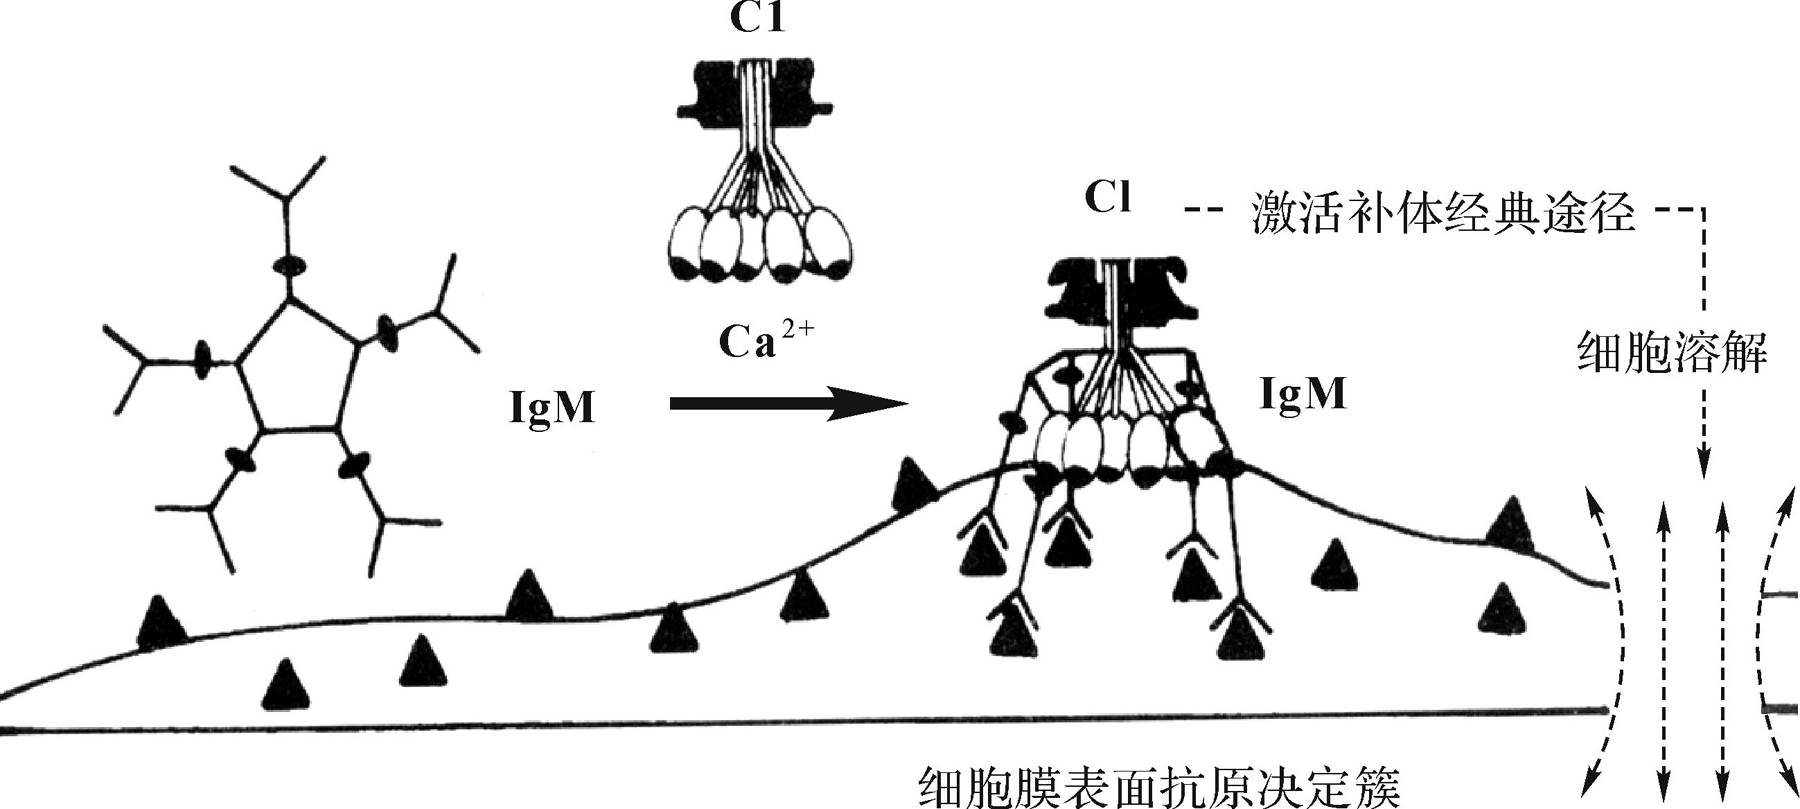
\includegraphics[width=.6\textwidth]{./images/Image00182.jpg}
 \captionsetup{justification=centering}
 \caption{直接溶血空斑试验作用机制示意图}
 \label{fig10-28}
  \end{figure} 

(2)间接溶血空斑试验法:检测分泌IgG或其他类别Ig的抗体形成细胞。

方法:前两步与直接法相同,第三步需加入抗IgG或其他抗抗体,再加豚鼠新鲜补体进行观察(图\ref{fig10-29})。

\begin{figure}[!htbp]
 \centering
 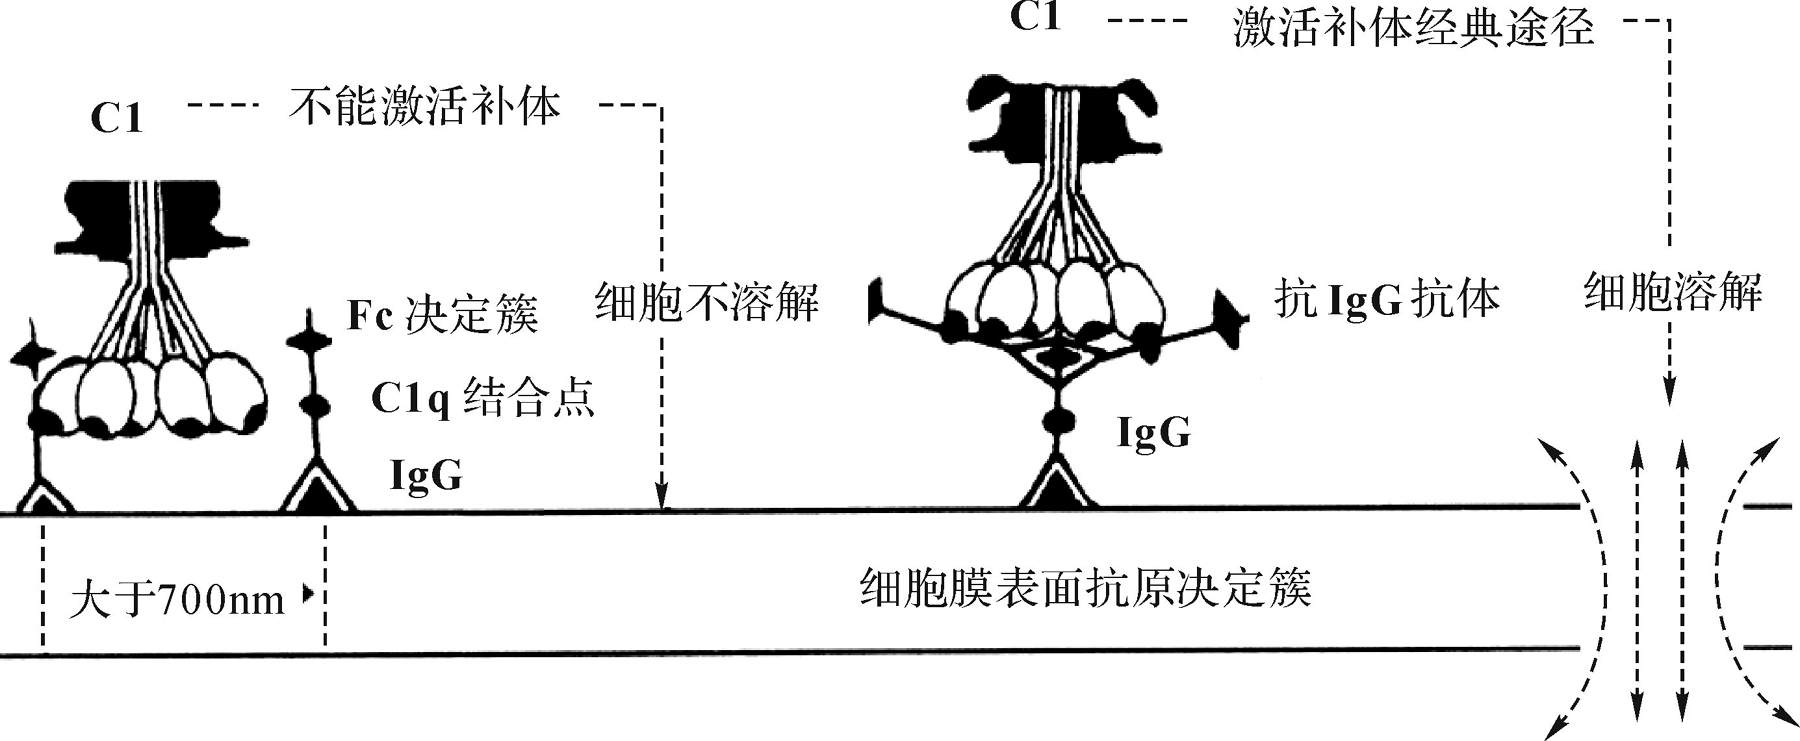
\includegraphics[width=.6\textwidth]{./images/Image00183.jpg}
 \captionsetup{justification=centering}
 \caption{间接溶血空斑试验作用机制示意图}
 \label{fig10-29}
  \end{figure} 

\section{检测体液和细胞免疫功能的体内试验}

皮肤试验是测定机体体液和细胞免疫状态的一种体内试验,用于过敏性疾病、传染病、免疫缺陷性疾病和肿瘤等的诊断、防治、疗效和预后的判定。


\subsection{检测体液免疫的皮肤试验}

(一)速发型超敏反应皮肤试验

注射青霉素、普鲁卡因、抗毒素血清等均需进行皮肤试验,以判定体内特异性IgE产生情况和机体的致敏状态。

方法:青霉素100U/mL,抗毒素血清1∶1000,取0.1mL皮内注射,20分钟内观察结果。

结果:皮肤红晕水肿,直径大于1cm,为“+”。

(二)毒素皮肤试验

1.狄克试验(又称红疹毒素皮肤试验)

红疹毒素是A族链球菌产生的一种外毒素,是引起猩红热皮疹的主要物质。

试验目的:测定机体对猩红热是否易感,检测体内是否具有红疹毒素抗体。

方法:0.1mL红疹毒素注射于前臂皮内,6~24h后观察。

(1)皮肤红斑直径大于1cm,是“+”,表明受试者体内没有相应抗毒素,对猩红热易感。

(2)局部皮肤不出现红疹------说明注入的红疹毒素已被相应的抗毒素中和,机体对猩红热有抵抗力,不易感。

2.锡克试验------检测机体对白喉免疫力的皮肤试验

方法和结果判定与狄克试验大致相同。注射白喉毒素后24~48h。

(1)局部皮肤红肿“+”------表明受试者体内没有相应抗毒素,对白喉无免疫力。

(2)局部皮肤不红肿------表明白喉毒素被相应抗体中和,机体对白喉有一定的免疫力。

鉴于有人对白喉毒素有超敏反应,试验时应取另一份白喉毒素 80℃ 5min
破坏毒性,注射于受试者另一前臂皮内作为对照。


\subsection{检测细胞免疫功能的皮肤试验}

检测细胞免疫功能的皮肤试验是根据迟发型超敏反应(即细胞免疫反应)的发生机制建立的。抗原注入皮内,经48~72小时观察结果。

(1)局部皮肤红肿、硬结、直径大于0.5cm,为“+”,表明细胞免疫功能正常。

(2)反应微弱或皮试阴性,表明细胞免疫功能低下。

用途:(1)某些传染病和免疫缺陷病的诊断,(2)观测肿瘤治疗的效果和判断其预后。

常用生物性抗原有:结核菌素(OT)、结核菌纯蛋白衍生物(PPD)、念珠菌素、链激酶-链道酶(SK-SD)和植物性血凝素(PHA)等。

\noindent\textbf{【理解与思考】}

1.从血清学试验的一般规律看抗原、抗体检测的实质是什么?你能科普性地描述检测方法吗?

2.体内检测试验的实质是什么?医学上还有哪些体内试验?

3.请将免疫检测与前面几章内容联系起来,如果要检测诸如抗原、抗体、MHC、补体、细胞因子等,该如何检测?为什么?

\noindent\textbf{【课外拓展】}

1.其他免疫检测方法还有哪些?

2.如何检测细胞因子的种类及其活性?

\noindent\textbf{【课程实验与研究】}

1.设计一个用免疫方法检测某种细菌的实验。

2.设计一种鉴别不同淋巴细胞的实验方法。

3.临床上是如何检测肿瘤抗原的?请设计几种不同的方法检测甲胎蛋白,并请比较其敏感性。

4.《Science》最近报道称发现一类新T细胞。请设计一种方案,鉴别出它不是已经发现的免疫细胞中的一种。

5.《PNAS》报道称“发现保护动物抵抗禽流感新蛋白”,请就它的结构、分子量、生物学活性提出检测方案。

6.法国马赛Mediterranean Aix-Marseille 大学的病毒学家Xavier de
Lamballerie在2009年年末表示:开展血清抗体测试研究,揭示甲型H1N1流感真实感染数据。请你为研究设计一个方案。

\noindent\textbf{【课程研讨】}

1.如果要确诊某种病原微生物或是否得了某种传染病,请设计多种检测方法。并请比较你们小组所设计不同方法的优劣。

2.要检测食品中是否有三聚氰胺,能用免疫检测的方法吗?如可行,请设计检测方法;如不行,说明理由。

3.免疫学检测除了用于医学、生物学,你认为还能用在哪些领域?说明机理。

4.请就免疫检测的最新进展写一篇综述。

\noindent\textbf{【课后思考】}

1.凝集试验、免疫标记技术、酶联免疫吸附试验(ELISA)的概念。

2.试述抗原或抗体检测的应用。

\noindent\textbf{【课外阅读】}

\begin{center}
 \textbf{\Large 严重急性呼吸道综合征的实验室检查}
 \end{center}

SARS的诊断主要依据起病急、高热、咳嗽及X线胸片显示肺部浸润性改变等临床表现,结合流行病学史以及必要的实验室检查。目前,较为特异的实验室诊断技术有以下几种:

1.分子学检测

许多病毒感染性疾病早期病毒分泌最多,但是在SARS的发病初期,SARS-CoV含量非常少,需要用非常敏感的手段才能检测到低水平的病毒核酸,主要用反转录-聚合酶链反应(reverse
transcrip-tion polymerase chain
reaction,RT-PCR)或实时聚合酶链反应(real-time
PCR)检测可疑和发病患者的呼吸道分泌物、血液、尿液或粪便等人体标本中的病毒。鼻咽部分泌物为最适用标本,多部位标本联合检测可提高阳性率。Real-time
PCR灵敏度极高,可以检测到单个拷贝的病毒基因。但是由于受引物特异性、检测样本采集时间、种类及其处理方法、病毒核酸在样本中的含量以及样本中的酶抑制物等因素的影响,仍有假阴性结果出现。因此,PCR检测结果阴性,并不能确定该患者没有感染SARS-CoV。

2.血清学检测

已建立的检测病人血清抗体的方法有免疫荧光( immunofluorescence
assay,IFA)和酶联免疫吸附试验(enzyme linked immunoabsorbent
assay,ELISA)。血清抗体的研究表明,SARS患者发病后,最早的IgM抗体要在7天左右出现,10天时达到高峰,15天左右下降;抗体IgG
10天后产生,20天左右达到高峰。IFA检测可以检测出SARS-CoV感染10天后患者血清中产生的IgM。ELISA法要在SARS患者出现临床症状21天左右才可检测到稳定的IgG。SARS感染血清学诊断双份血清标本最可靠,故应尽可能采取进展期的标本。IFA检测时应将双份血清标本置于同一张玻片,ELISA检测时应将双份血清标本置于同一块酶免疫反应板内,这样检测的滴度才有可比性。通过这两种不同的血清抗体快速诊断试剂检测,可以鉴别患者是新感染还是曾经有过冠状病毒感染,病人是否产生相应的抗体。但是一般患者在患病初期,血液里虽有病毒,但抗体可能还没有形成,检测结果呈阴性;有时SARS病毒处于潜伏期,尚未出现症状或症状不典型,此时检测结果也是阴性。所以,这两种方法不适合早期诊断。

3.病毒检测

病毒的分离鉴定是确立病原学诊断的“金标准”。同其他冠状病毒不同,SARS-CoV很容易在体外33~37℃培养。利用VERO
E6或VERO细胞(从成年长尾猿属的非洲绿猴肾中提取的一种细胞系)来培养或扩增SARS患者的呼吸道分泌物、尿液粪便和血液样品,分离得到的病毒可以进一步验证是否为SARS-CoV。细胞感染24小时即可出现病变。培养细胞进行电镜观察可以确定冠状病毒,但不能肯定是SARS-CoV,最后诊断仍需要通过SARS-CoVRNA的PCR检测或全基因组测序。因此,病毒分离不能快速检测,而且细胞培养阴性也不能排除SARS。因为SARS-CoV为高度传染性,只允许在生物安全水平3级或以上的实验室进行,加上体外细胞培养分离十分复杂和繁琐,所以病毒检测对一般的临床实验室来说并不是一种常规的检测方法。

\begin{center}
 \textbf{\Large 中国体外诊断行业概况}
 \end{center}

体外诊断产业,就是指在人体之外通过对人体的血液等组织及分泌物进行检测获取临床诊断信息的产品和服务,在国际上统称IVD(In-Vitro
Diagnostics
)产业。IVD产业与检验医学构成了既相互区别又相互紧密联系的有机整体,体外诊断产业是检验医学的“工具”和“兵器”,同时检验医学是体外诊断产业的“用户”和“市场”,两者的共同目的是实施体外诊断。有专家指出,临床诊断信息的80\%左右来自体外诊断,而其费用占医疗费用不到20\%。体外诊断已经成为人类疾病预防、诊断、治疗日益重要的组成部分,是保障人类健康与构建和谐社会日益重要的组成部分。

我国体外诊断产业的发展开始于20世纪80年代,经历20多年的发展,从无到有,从弱到强,现正处于快速增长阶段。从市场角度看,我国是人均消费最低的国家之一,中国以世界1/5的人口,占据全世界IVD产业2\%左右的市场份额,2007年全国市场规模在100亿元人民币左右。但是,中国同时是市场增长速度最快的国家,年均增长率在15\%~20\%。我国IVD用户主要包括1800多家医院、300多家血站,还有日新月异的体检中心,正在兴起的临床检验独立实验室。如果我国城镇居民的医疗水平接近美国全国居民的医疗水平,则我国IVD
产业的市场规模将扩大20倍。从制造商或供应商角度看,在我国主要有三类制造商:一类是世界著名的跨国公司,包括IVD产业世界十强,如GE(美国通用)、西门子、罗氏、强生、倍克曼、德林等公司;一类是民族企业中的知名企业,如在香港上市的中生北控生物科技股份有限公司,在国内上市的上海科化、广州达安,在纽约证券所上市的深圳迈瑞等;一类是新兴或中小型的其他民族企业,由于恶性竞争的存在,行业总体赢利水平目前降至10%-20%,企业数量每天都在变化,但总数在1000家左右。从产品上看,目前在临床应用比较广泛、市场广阔的项目上(如免疫试剂中的肝炎、性病和孕检系列,临床生化中的酶类、脂类、肝功、血糖、尿检等系列),国内主要生产厂家的技术水平已基本达到国际同期水平;基因检测中的PCR技术系列已经基本达到国际先进水平,基因芯片、癌症系列正在开始迅速追赶国际水平。从市场环境角度看,法规从无到有,正在借鉴发达国家的成功经验和结合本国国情的原则指导下完善,而用户方面普遍对价格敏感,消费能力不同地区发展不平衡,城乡差别明显。

在2008年新医改政策及国家4万亿放量刺激内需的环境变化下,体外诊断行业面临前所未有的巨大机遇。不仅国内的体外诊断试剂和仪器生产企业,外国资本亦表现出了浓厚兴趣。典型例子是,2008年11月初北京科美东雅生物技术有限公司完成了第二轮高达1650万美元的私募融资,这为其拓展以化学发光(CLIA)体外诊断产品为核心的市场营销网络,进一步确立其IVD品牌实力提供了强大的资金实力。

